 % The main file for CAMP reports
 % Don't put any content in here. 
 % Don't even include content files by using \input or \inlcude. 
 % Put your content to TEXT.TEX or include it there using \input.
 % Uses:
 %              SETTINGS.TEX    contains the settings for this document
 %              COMMANDS.TEX    contains commands which can be used while writing
 %              INFO.TEX                        contains the author, title and so on for the cover
 %              COVER.TEX                       formats the front cover of the document
 %              ABSTRACT.TEX    contains the abstract to be included (if needed)
 %              TEXT.TEX                        contains the actual content of the document
 %              BIB.BIB                         containt the BibTeX entries for the document
 
 
%% Draft document mode
%% Final document
\documentclass[11pt,a4paper,bibtotoc,idxtotoc,headsepline,footsepline,footexclude,BCOR12mm,DIV13]{scrbook}

%\documentclass[11pt,a4paper,bibtotoc,idxtotoc,headsepline,footsepline,footexclude,BCOR20mm,DIV10]{scrbook}

% KOMA-Optionen:
%  bibtotoc: include bibliography in table of contents
%  idxtotoc: include index in table of contents
%  headsepline: use horizontalline under heading
%  BCOR: binding correcion (Bindungskorrektur) (e.g.: BCOR5mm)
%  DIV: Number of sheet sections (used for layout) (e.g.: DIV12) 



% include title and author information for the cover
% Set here the title, authors and other stuff to be used for the cover
% This file is used by MAIN.TEX

% set title, authors and stuff for the cover
\def\doctype{Master's Thesis}
\def\title{Implementation of Contracting Curve Density Algorithm for Applications in Personal Robotics}
\def\titleGer{Durchführung von Contracting Curve Density-Algorithmus für Anwendungen in der Robotik Personal}
\def\author{Shulei Zhu}
\def\date{April 1, 2011}

% text to appear in the footer
\def\footertext{}

% include settings
% Included by MAIN.TEX
% Defines the settings for the CAMP report document

\renewcommand{\sectfont}{\normalfont \bfseries}        % Schriftart der Kopfzeile

% manipulate footer
\usepackage{scrpage2}
\pagestyle{scrheadings}
\ifoot[\footertext]{\footertext} % \footertext set in INFO.TEX
%\setkomafont{pagehead}{\normalfont\rmfamily}
\setkomafont{pagenumber}{\normalfont\rmfamily}

%% allow sophisticated control structures
\usepackage{ifthen}

% use Palatino as default font
\usepackage{palatino}

% enable special PostScript fonts
\usepackage{pifont}

% make thumbnails
\usepackage{thumbpdf}

%to use the subfigures
\usepackage{subfigure}


\usepackage{colortbl}


%% show program code\ldots
%\usepackage{verbatim}
%\usepackage{program}

%% enable TUM symbols on title page
\usepackage{styles/tumlogo}


\usepackage{multirow}

%% use colors
\usepackage{color}

%% make fancy math
\usepackage{amsmath}
\usepackage{amsfonts}
\usepackage{amssymb}
\usepackage{textcomp}
\usepackage{yhmath} % f�r die adots 
%% mark text as preliminary
%\usepackage[draft,german,scrtime]{prelim2e}

%% create an index
\usepackage{makeidx}

% for the program environment
\usepackage{float}

%% load german babel package for german abstract
%\usepackage[german,american]{babel}
\usepackage[german,english]{babel}
\selectlanguage{english}

% use german characters as well
\usepackage[latin1]{inputenc}       % allow Latin1 characters

% use initals dropped caps - doesn't work with PDF
\usepackage{dropping}


\usepackage{styles/shortoverview}
%----------------------------------------------------
%      Graphics and Hyperlinks
%----------------------------------------------------

%% check for pdfTeX
\ifx\pdftexversion\undefined
 %% use PostScript graphics
 \usepackage[dvips]{graphicx}
 \DeclareGraphicsExtensions{.eps,.epsi}
 \graphicspath{{figures/}{figures/review}} 
 %% allow rotations
 \usepackage{rotating}
 %% mark pages as draft copies
 %\usepackage[english,all,light]{draftcopy}
 %% use hypertex version of hyperref
 \usepackage[hypertex,hyperindex=false,colorlinks=false]{hyperref}
\else %% reduce output size \pdfcompresslevel=9
 %% declare pdfinfo
 %\pdfinfo { 
 %  /Title (my title) 
 %  /Creator (pdfLaTeX) 
 %  /Author (my name) 
 %  /Subject (my subject	) 
 %  /Keywords (my keywords)
 %}
 %% use pdf or jpg graphics
 \usepackage[pdftex]{graphicx}
 \DeclareGraphicsExtensions{.jpg,.JPG,.png,.pdf,.eps}
 \graphicspath{{figures/}} 
 
 %% Load float package, for enabling floating extensions
 \usepackage{float}
 
 %% allow rotations
 \usepackage{rotating}
 %% use pdftex version of hyperref
 \usepackage[pdftex,colorlinks=true,linkcolor=red,citecolor=red,%
 anchorcolor=red,urlcolor=red,bookmarks=true,%
 bookmarksopen=true,bookmarksopenlevel=0,plainpages=false%
 bookmarksnumbered=true,hyperindex=false,pdfstartview=%
 ]{hyperref}
%
%\usepackage[pdftex,colorlinks=false,linkcolor=red,citecolor=red,%
% anchorcolor=red,urlcolor=red,bookmarks=true,%
% bookmarksopen=true,bookmarksopenlevel=0,plainpages=false%
% bookmarksnumbered=true,hyperindex=false,pdfstartview=%
% ]{hyperref}
\fi




%% Fancy chapters
%\usepackage[Lenny]{fncychap}
%\usepackage[Glenn]{fncychap}
%\usepackage[Bjarne]{fncychap}

%\usepackage[avantgarde]{quotchap}

% set the bibliography style
%\bibliographystyle{styles/bauermaNum}
%\bibliographystyle{alpha}
\bibliographystyle{plain}

% include commands
% Commands to be used within the TUM report document
% Included by MAIN.TEX
% Please include your own cool commands here. 
% Be only sure to comment it sufficiently so others can use it.

%-------------------------------------------------------------
%                      Own Commands
%-------------------------------------------------------------


%-------------------------------------------------------------
% math stuff -------------------------------------------------

% nice R, N, C
\newcommand{\nat}{\mathbb{N}}
\newcommand{\real}{\mathbb{R}}
\newcommand{\compl}{\mathbb{C}}



% norm
\newcommand{\norm}[1]{\left\| #1 \right\|}

% un demi
\newcommand{\half}{\frac{1}{2}}

% parantheses
\newcommand{\parenth}[1]{ \left( #1 \right) }
\newcommand{\bracket}[1]{ \left[ #1 \right] }
\newcommand{\accolade}[1]{ \left\{ #1 \right\} }
%\newcommand{\angle}[1]{ \left\langle  #1 \right\rangle }

% partial derivative: %#1 function, #2 which variable
% simple / single line version
\newcommand{\pardevS}[2]{ \delta_{#1} f(#2) }
% fraction version
\newcommand{\pardevF}[2]{ \frac{\partial #1}{\partial #2} }

% render vectors: 3 and 4 dimensional
\newcommand{\veciii}[3]{\left[ \begin{array}[h]{c} #1 \\ #2 \\ #3       \end{array} \right]}
\newcommand{\veciv}[4]{\left[ \begin{array}[h]{c} #1 \\ #2 \\ #3 \\ #4  \end{array} \right]}

% render matrices: 3  dimensional (arguments in row first order)
\newcommand{\matiii}[9]{\left[ \begin{array}[h]{ccc} #1 & #2 & #3 \\ #4 & #5 & #6 \\ #7 & #8 & #9       \end{array} \right]}
%DOESN'T WORK,DON'T KNOW WHY \newcommand{\mativ}[16]{\left[ \begin{array}[h]{cccc} #1 & #2 & #3 & #4 \\ #5 & #6 & #7 & #8 \\ #9 & #10 & #11 & #12 \\ #13 & #14 & #15 & #16 \end{array} \right]}


%-------------------------------------------------------------
%-------------------------------------------------------------


%-------------------------------------------------------------
% some abreviations ------------------------------------------
\newcommand{\Reg}{$^{\textregistered}$}
\newcommand{\reg}{$^{\textregistered}$ }
\newcommand{\Tm}{\texttrademark}
\newcommand{\tm}{\texttrademark~}
\newcommand {\bsl} {$\backslash$}

%-------------------------------------------------------------
%-------------------------------------------------------------


%-------------------------------------------------------------
% formating --------------------------------------------------

% Theorem & Co environments and counters
\newtheorem{theorem}{Theorem}[chapter]
\newtheorem{lemma}[theorem]{Lemma}
\newtheorem{corollary}[theorem]{Corollary}
\newtheorem{remark}[theorem]{Remark}
\newtheorem{definition}[theorem]{Definition}
\newtheorem{equat}[theorem]{Equation}
\newtheorem{example}[theorem]{Example}
% \newtheorem{algorithm}[theorem]{Algorithm}

% inserting figures
\newcommand{\insertfigure}[4]{ % Filename, Caption, Label, Width percent of textwidth
        \begin{figure}[htbp]
                \begin{center}
                        \includegraphics[width=#4\textwidth]{#1}
                \end{center}
                \vspace{-0.4cm}
                \caption{#2}
                \label{#3}
        \end{figure}
}




% referecing figures

\newcommand{\refFigure}[1]{ %label
        figure \ref{#1}
}
\newcommand{\refChapter}[1]{ %label
        chapter \ref{#1}
}

\newcommand{\refSection}[1]{ %label
        section \ref{#1}
}

\newcommand{\refParagraph}[1]{ %label
        paragraph \ref{#1}
}

\newcommand{\refEquation}[1]{ %label
        equation \ref{#1}
}

\newcommand{\refTable}[1]{ %label
        table \ref{#1}
}




\newcommand{\rigidTransform}[2]
{
        ${}^{#2}\!\mathbf{H}_{#1}$
}

%code, in typewriter
\newcommand{\code}[1]
 {\texttt{#1}}

% comment that appears on the border - very practical !!!
\newcommand{\comment}[1]{\marginpar{\raggedright \noindent \footnotesize {\sl #1} }}

% page clearing
\newcommand{\clearemptydoublepage}{%
  \ifthenelse{\boolean{@twoside}}{\newpage{\pagestyle{empty}\cleardoublepage}}%
  {\clearpage}}


%-------------------------------------------------------------
%-------------------------------------------------------------


\newcommand{\etAl}{\emph{et al.}\mbox{ }}



%\makeindex
        %% inter line spacing
%\linespread{1.0}

\makeglossary

\begin{document}

        \frontmatter
        
        
        % The front cover for the TUM report document.
% Included by MAIN.TEX


%--------------------------------------------------
% The Front Cover
%--------------------------------------------------

% The front cover for the TUM document.
% Included by MAIN.TEX


%--------------------------------------------------
% The Front Cover
%--------------------------------------------------

% correct BCOR - undo at the end !!!
\def\bcorcor{0.15cm}
\addtolength{\hoffset}{\bcorcor}

\thispagestyle{empty}

 \vspace{4cm}
\begin{center}
               \oTUM{4cm}\\          
           \vspace{0.5cm}
         \large Technischen Universit{\"a}t M{\"u}nchen\\
    \vspace{1mm}
    \large Computational Science and Engineering (Int. Master's Program)
    \vspace{1mm}
  \end{center}
               
  \vspace{10mm}

\begin{center}  

  {\Large \doctype}

  \vspace{10mm}
  
  {\LARGE \title}\\
  \vspace{10mm}
  {\LARGE \author}\\
  
  \vspace{10mm}
  
  \vspace{10mm}

    %\hfill
    \begin{tabular}{ll}
           \Large 1st examiner:    & \Large  Beetz, Michael; Prof. PhD. \\[2mm]                                
           \Large 2nd examiner:      & \Large Hans-Joachim, Bungartz; Prof. Dr. \\[2mm]
           \Large Assistant advisor:  & \Large Pangercic, Dejan; M.Sc.\\[2mm]
           \Large Thesis handed in on:       & \Large April 20, 2011
         \end{tabular}
         
         \vspace{5mm}
         
         \begin{figure}[h!]
  \centering
   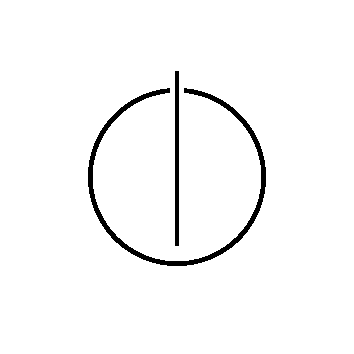
\includegraphics[width=4cm]{styles/informat.png}
  \end{figure}
   

\end{center}

%       \clearemptydoublepage
%       
%       % The titlepage for the CAMP report document.
% Included by MAIN.TEX


%--------------------------------------------------
% The title page
%--------------------------------------------------

% correct BCOR - undo at the end !!!
\def\bcorcor{0.15cm}
\addtolength{\hoffset}{\bcorcor}

\thispagestyle{empty}

 \vspace{10mm}
\begin{center}
               \oTUM{4cm}
           
           \vspace{5mm}     
           \huge FAKULT{\"A}T F{\"U}R INFORMATIK\\ 
           \vspace{0.5cm}
         \large DER TECHNISCHEN UNIVERSIT{\"A}T M{\"U}NCHEN\\
        
        \end{center}
                

\vspace{10mm}
\begin{center}

   {\Large \doctype}

  \vspace{10mm}
  
  {\LARGE \title}\\
  
  
  \vspace{10mm}
  
  
  {\LARGE  \titleGer}\\
  
  
  \vspace{10mm}

    %\hfill
    \begin{tabular}{ll}
           \Large Author:     & \Large \author \\[2mm]
           \Large Supervisor:    & \Large  Beetz, Michael; Prof. \\[2mm]                                
           \Large Advisor:      & \Large M.Sc. Pangercic, Dejan\\[2mm]
           \Large Date:       & \Large April 1, 2011
         \end{tabular}
         
         \vspace{5mm}
         
         \begin{figure}[h!]
  \centering
   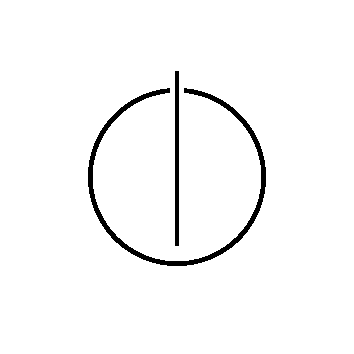
\includegraphics[width=4cm]{styles/informat.png}
  \end{figure}
   

\end{center}

% undo BCOR correction
\addtolength{\hoffset}{\bcorcor}
        
        
%       \input{components/cover_maschmeyer}
        % \clearemptydoublepage
        
        % % The titlepage for the CAMP report document.
% Included by MAIN.TEX


%--------------------------------------------------
% The title page
%--------------------------------------------------

% correct BCOR - undo at the end !!!
\def\bcorcor{0.15cm}
\addtolength{\hoffset}{\bcorcor}

\thispagestyle{empty}

 \vspace{10mm}
\begin{center}
               \oTUM{4cm}
           
           \vspace{5mm}     
           \huge FAKULT{\"A}T F{\"U}R INFORMATIK\\ 
           \vspace{0.5cm}
         \large DER TECHNISCHEN UNIVERSIT{\"A}T M{\"U}NCHEN\\
        
        \end{center}
                

\vspace{10mm}
\begin{center}

   {\Large \doctype}

  \vspace{10mm}
  
  {\LARGE \title}\\
  
  
  \vspace{10mm}
  
  
  {\LARGE  \titleGer}\\
  
  
  \vspace{10mm}

    %\hfill
    \begin{tabular}{ll}
           \Large Author:     & \Large \author \\[2mm]
           \Large Supervisor:    & \Large  Beetz, Michael; Prof. \\[2mm]                                
           \Large Advisor:      & \Large M.Sc. Pangercic, Dejan\\[2mm]
           \Large Date:       & \Large April 1, 2011
         \end{tabular}
         
         \vspace{5mm}
         
         \begin{figure}[h!]
  \centering
   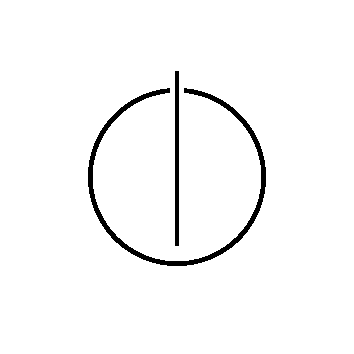
\includegraphics[width=4cm]{styles/informat.png}
  \end{figure}
   

\end{center}

% undo BCOR correction
\addtolength{\hoffset}{\bcorcor}
        
        
        \clearemptydoublepage


\thispagestyle{empty}
\selectlanguage{german}
        \vspace*{0.8\textheight}
        \noindent
        I hereby declare that this thesis is entirely the result of my
        own work except where otherwise indicated. I have only used
        the resources given in the list of references.\\
        
        \vspace{15mm}
        \noindent
        M{\"u}nchen, den \today \hspace{5cm} \author
\selectlanguage{english}
\newpage
        
        \clearemptydoublepage
\phantomsection
\addcontentsline{toc}{chapter}{Acknowledgements}        


%\chapter*{Acknowledgements}

\vspace*{2cm}

\begin{center}
{\Large \bf Acknowledgments}
\end{center}

\vspace{1cm}




Here I would like to express my gratitude to all people who supported me during the
progress of this work. Especially I would like to thank:

Prof. Beetz PhD. for giving me the opportunity to work on this thesis;

Prof. Hans-Joachim Bungartz for his efforts to examine this work;

Dejan Pangercic, for the supervision of my thesis, for his planning and instructions,
for his countless ideas, suggestions, efforts and assistances, for his help and care for
my life;

Dr. Giorgio Panin for explainations regarding the CCD algorithm;

Zoltan Csaba Marton for his suggestions and helpful discussions;

Goron Lucian for his suggestions, corrections and other assistances;

Andrei Haidu, Ferko for their corrections;

Dr. Robert Hanek for his help and suggestions;

Of course special thanks go to my parents and my brother without whom this work
would not have been possible and for supporting me in every way possible.

Last, but certainly not least, I would like to thank xxxx, who supported me with her
love, encouragement, and assistances in many ways.


        
        % Abstract for the TUM report document
% Included by MAIN.TEX


\clearemptydoublepage
\phantomsection
\addcontentsline{toc}{chapter}{Abstract}        





\vspace*{2cm}
\begin{center}
{\Large \bf Abstract}
\end{center}
\vspace{1cm}

% This master's thesis investigates an extended and optimized
% implementation of a state-of-the-art local curve fitting algorithm,
% the Contracting Curve Density (CCD).
% In particular, we investigate
% the application of the CCD algorithm and its variant the CCD tracker
% on personal robotics (e.g. PR2).

% We developed an application based on the OpenCV library, which
% is a cross-platform computer vision library. Based on the
% design conception of the CCD algortihm, some
% additional features are integrated into the developed program in order to
% achieve stability and robustness. Firstly, we use the logistic sigmoid
% function instead of Gaussian error function, thus completely convert a
% curve-fitting problem to a Gaussian logistic regression problem in the
% field of pattern recognition. Secondly, the quadratic (degree-2) or
% cubic (degree-3) B-spline curve is used to model the parametric curve
% to avoid the Runge phenomenon without increasing the degree of the
% B-spline. Thirdly, the system supports both planar affine (6-DOF) and
% non-planar affine (8-DOF) shape-space. The extended affine space can avoid
% curve mismatching caused by minor viewpoint changes. Moreover, in
% order to avoid manual intervention from the user, the developed system
% also supports robust global initialization modules based on both keypoint
% feature matching and 3-Dimensional point cloud. At last, the CCD
% algorithm solves the curve fitting problem by converting it to a
% pattern recognition problem, and because maximum a posteriori probability
% (MAP) estimate is an important but time-cost step. We proposed some
% changes and optimization on it.

% The developed system mainly consists of two functional parts, the CCD
% algorithm to fit model curve in still images and the CCD tracker to
% track model in sequential-frame video. We apply the CCD algorithm to
% serval image segmentation and object tracking problems. Some experiments with RGB
% images and videos are delivered on Personal Robot 2 (PR2), and the
% performance is examined on two tasks listed above.  It is shown that
% the CCD algorithm achieves robustness and subpixel accuracy even in the
% presence of clutter, partial occlusion, and changes of
% illumination. We present results for some curve-ftting problems, such
% as image segmentation, 3-D pose estimation, object tracking based on
% both manual intervention and automatical initialization.

This thesis investigates an extended and optimized
implementation of the state-of-the-art local curve fitting algorithm
named Contracting Curve Density (CCD) algorithm, originally developed 
by Hanek et al. In particular, we investigate its application  
in the field of personal robotics for the tasks such as the segmentation
of objects in clutter and the tracking of objects. 

The CCD algorithm can be best described as follows. Given one or multiple images as input
data and a parametric curve model with a priori distribution of model
parameters, through curve-fitting process, we estimate the model
parameters which determine the approximation of the posterior
distribution in order to make the curve models best matching the image data.
In order to improve the stability, accuracy and robustness over the original
implementation we introduce the following improvements. Firstly, we use the logistic sigmoid
function instead of a Gaussian error function which renders a
curve-fitting problem as a Gaussian logistic regression problem known in the
field of pattern recognition. Secondly, a quadratic or
a cubic B-spline curve is used to model the parametric curve
to avoid the Runge phenomenon without increasing the degree of the
B-spline. Thirdly, the system supports both planar affine (6-DOF) and
three-dimensional affine (8-DOF) shape-space. The latter affine space can avoid
curve mismatching caused by major viewpoint changes. Lastly, in
order to avoid manual intervention by the user, the developed system
also supports robust global initial curve initialization modules based on both keypoint
feature matching and back-projections from the 3D point clouds. 

The developed system mainly consists of two functional parts, the CCD
algorithm to fit the model curve in still images and the CCD tracker to
track the model in the videos. We demonstrate algorithm's working 
in various scenes using handheld camera and the cameras from the 
PR2 robot. Achieved results show that the CCD algorithm achieves 
robustness and sub-pixel accuracy even in the presence of clutter, 
partial occlusion, and changes of illumination. 














        \tableofcontents
  
  % \clearemptydoublepage

\phantomsection
\addcontentsline{toc}{chapter}{Outline of the Thesis}

\begin{center}
	\huge{Outline of the Thesis}
\end{center}




%--------------------------------------------------------------------
\section*{Part I: Introduction and Theory}

\noindent {\scshape Chapter 1: Introduction}  \vspace{1mm}

\noindent  This chapter presents an overview of the thesis and it purpose. Furthermore, it will discuss the sense of life in a very general approach.  \\

\noindent {\scshape Chapter 2: Theory}  \vspace{1mm}

\noindent  No thesis without theory.   \\

%--------------------------------------------------------------------
\section*{Part II: The Real Work}

\noindent {\scshape Chapter 3: Overview}  \vspace{1mm}

\noindent  This chapter presents the requirements for the process.

        \mainmatter

                \chapter{Introduction}
\label{chapter:Introduction}
In the field of computer vison and pattern recognition, determining a
model from a finite set of samples or a complex image without a prior
knowledge is an ill-posed problem. Due to the the ill-posedness, in
the sense that a unique model may not exist, models specifying a prior
knowledge play a very important role in solving many important
computer vision problems, such as object tracking, shape recognition,
pose estimation, segmentation, edge detection, stereo matching and 3-D
reconstruction.

Some parametric curve models, also known as deformable models,
deformable templates, Snakes, or active contours, have been developed
to guide the image interpretation process towards particularly
likely interpretations~\cite{hanek2004fitting}. These parametric curve
models have had two outstanding influences on the
development of related algorithms. The first is the Snakes which
represent a fundamentally new framework for delineating an object
outline in an image. This algorithm attempts to minimize energy
associated to the current contour as a sum of an internal and an external
energy~\cite{kass1988snakes}. The goal of Snakes is to balance the prior
knowledge with evidence from an image. The second outstanding
influence is in the field of pattern recognition and machine learning,
where statistical distributions play a key role.  There treatment
of a prior knowledge about shape is put into a probabilistic
context. Any shape is regarded as the result of applying some
distortion to an ideal prototype shape, and an appropriate
distribution governs the nature and extent of that distortion.
For both kinds of methods, the common aim is to strengthen the visual
interpretation of the shape via the establishing influence of prior
expectations of the shapes that are likely to be
seen~\cite{blake1998active}. This thesis dwells upon the Contracting
Curve Density (\acronym{CCD}{Contracting Curve Density}) algorithm whose basic step is solving a
curve-fitting problem in a probabilistic context.


\section{The CCD Algorithm and Curve-fitting Problem}
\label{sec:ccdcfp}
The curve-fitting is a process that makes
a practical deformable template (model) attached to the feature in a
image. In essence it involves using algorithms to find the parameter
values for a given parametric curve model. Lots of important and
challenging computer vision tasks can be formulated as variants of the
curve-fitting problem. 

Suppose we have an observed object in an
image. Boundaries of the object can be completely or partially defined
by an either open or closed contour obtained by human intervention or
some object recognition techniques, such as \acronym{SIFT}{Scale-invariant feature transform} features or reconstruction. The goal of
the curve-fitting problem is to find the best visual fit of the contour to the boundary of
the observed object. Since the approximate boundaries of the observed
object have been given by the prior contour, there is no need to organise or group features in the
image, thus the analysis can be restricted to a relatively narrow
region of interest (\acronym{ROI}{Region of Interest}) and, as a result, performances of such algorithms
are boosted up. In the resulting ROI, we aim to distort the contour in a specific
shape-space and make it attach to the boundary of a given
object. There are many methods which can be used to cope with the
curve-fitting problem, the CCD approach discussed in this
thesis is a powerful model-based algorithm to solve it.

The CCD algorithm can be described as follows: Given one or multiple images as input
data and a parametric curve model with a prior distribution of model
parameters, through curve-fitting process we estimate the model
parameters which determine the approximation of the posterior
distribution in order to make the curve models best matching the image data.
Fig.~\ref{fig:fitting} depicts a curve-fitting problem and the corresponding solution obtained by the
CCD algorithm.
\begin{figure}[htb]
  \centering
  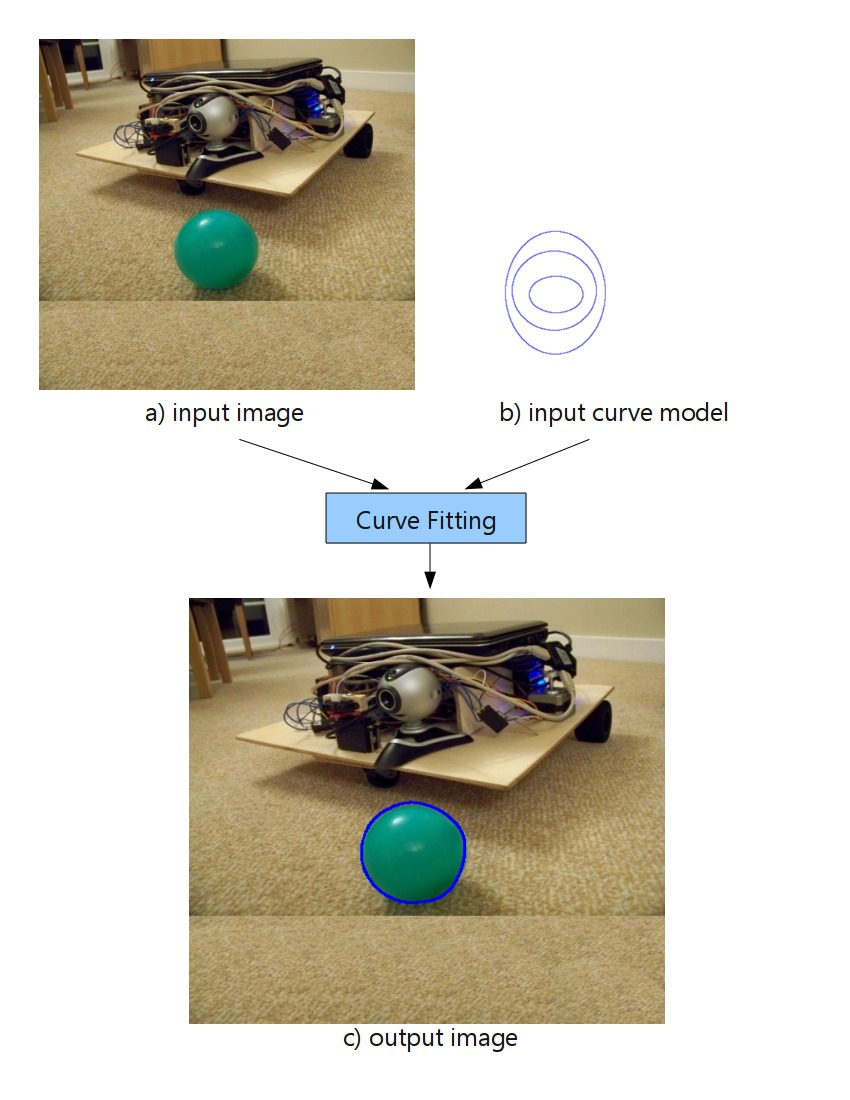
\includegraphics[width=10cm]{images/fitting.jpg}
  \caption[The description of curve-fitting problem]{The curve-fitting
    problem: a) an input
    image is given but not showing the pre-processing step. b) A series of
    parametric curve model contours which can be used to evaluate the
    prior distribution. These contours represent only a few possible
    shapes for the ball. c) The curve-fitting problem aims to estimate the model
    parameters by determining the posterior distribution. During the
    fitting process, the uncertainty of contours of the ball is widely
    reduced.}
  \label{fig:fitting}
\end{figure}

\section{Motivation For the CCD Algorithm}
\label{sec:mccd}
The curve-fitting problem and its variants have a wide range of
applications in the field of robotics, medical processing, user
interface, surveillance and biometrics~\cite{hanek2004fitting}. In order to be
widely applicable to practical personal robotics problems (such as
perception of mobile manipulation), robustness,
accuracy, efficiency and versatility should be
considered when a novel approach is designed and implemented.
However, in the computer vision community, solving object segmentation and the
related object contour tracking problems are always challenging,
especially in natural and unconstrained scenes. Due to clutter,
shading, texture, and highlights it is very difficult to segment
an object from an inhomogeneous background. Furthermore, some physical
conditions, such as the illumination or surface properties, will
influence the efficiency and stability of related approaches. It is
necessary and significant to develop a method which determines adequate segmentation
in advance or a single criterion that is applicable for all parts of objects boundaries.

Among the currently available methodologies, the CCD algorithm is
thought as the one that solves above problems best due to a high level
of robustness and sub-pixel accuracy even in the presence of severe
texture, shading, clutter, partial occlusion, and strong changes of
illumination and versatility. It is developed and presented as a state-of-the-art
improvement over other advanced techniques such as the condensation
algorithm~\cite{isard1998icondensation}. In the CCD approach, the curve-fitting problem is
put in the context of probabilistic framework and thus analogous to
the regression problem in the field of pattern recognition, which is especially
helpful to touch the nature of curve-fitting problem. By introducing
local image statistics, the algorithm can cope with highly
inhomogeneous image regions and provide therefore locally adapted
criteria for separating the adjacent image regions. The blurred
curve model is used as efficient means for iteratively optimizing the
posterior density over possible model parameters. It enables the
algorithm to trade-off two conflicting objectives, namely heaving a
large area of convergence and achieving high
accuracy~\cite{hanek2004fitting}.

The robustness, high performance and accuracy of the CCD algorithm enable it 
to be used on personal robot  because many applications in the field
of personal robotics are time-constrained. The object's contour
obtained by the CCD algorithm can be used to locate the object and 
establish a set of safe grasps on it~\cite{hanek2000vision}.

\section{The Contracting Curve Density (CCD) Algorithm}
\label{sec:sketch}

\subsection{An Alternative View of the CCD Algorithm}
\label{sec:overview}

In the field of pattern recognition, the key concept is that of
uncertainty. In image data, the uncertainty arises both
through noise from measurements, as well as through the nature of
the objects (e.g. cardiac motion and deformation). Probability theory
provides a consistent framework for the quantification and
manipulation of uncertainty.  In this section, we view curve-fitting
problem from a probabilistic perspective and turn us towards to
a classification problem.

In the CCD algorithm, we aim to find the contour of observed object
and thus segment it from the background. Therefore, a hypothetical 
contour divides the image into two part (Fig.\ref{fig:divide}), inside
and outside. For probabilistic model, we can represent this using
binary representation (e.g. $\{0, 1\}$). The goal of the CCD algorithm
is to accurately
assign a class label to each pixel in the image (Actually, we only need assign those pixels in the vicinity of the
contour), thus the curve-fitting problem becomes a classification
one. A powerful approach to solve this problem involves modeling a
conditional probability distribution in an inference stage, and then
subsequently uses this distribution to make optimal decisions. In
order to derive the conditional probability, prior distribution and
likelihood function should be given.

\begin{figure}[htbp]
  \centering
    \begin{minipage}[t]{0.5\linewidth} 
    \centering 
        \subfloat[]{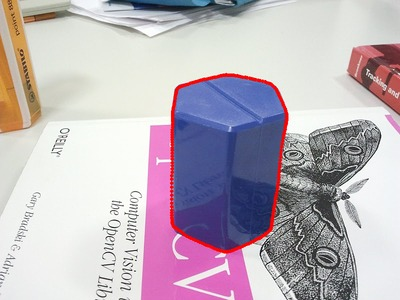
\includegraphics[width=8.0cm]{images/divide1.jpg}}
  \end{minipage}% 
  \begin{minipage}[t]{0.5\linewidth} 
    \centering 
    \subfloat[]{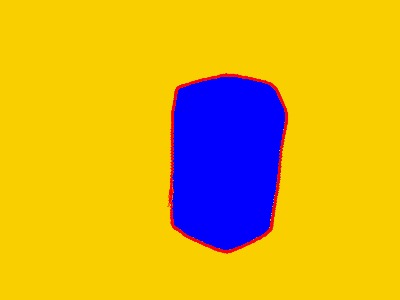
\includegraphics[width=8.0cm]{images/divide2.jpg}}
  \end{minipage} 
  \caption[A classification problem]{A classification problem: a) The red
    contour successfully segment the box from the background. b) The
    blue one is outside, the golden one is inside.}
  \label{fig:divide}
\end{figure}


We assume that a parametric curve model is governed by a prior distribution
over the model parameters (usually a multi-dimensional vector). There
exists a range of probability distributions which can be used to model
the distribution of shapes. In this thesis, for simplicity, let us
consider the Gaussian distribution, which is commonly used in computer
vison because of its several outstanding features. 


% \begin{equation}
%   \label{eq:1.1}
%   p(\mathbf{\Phi} | \mathbf{m}_{\mathbf{\Phi}}, \mathbf{\mathbf{\Sigma}}_{\mathbf{\Phi}}) = \mathcal{N}(\mathbf{\Phi} |
%   \mathbf{m}_{\mathbf{\Phi}},\mathbf{\Sigma}_{\mathbf{\Phi}}) =
%   \frac{1}{(2\pi )^{D/2}} \frac{1}{|\mathbf{\Sigma}_{\mathbf{\Phi}}|^{1/2}}
% \mathrm{exp} \left\{ -\frac{1}{2} (\mathbf{\Phi} -
%   \mathbf{\Sigma}_{\mathbf{\Phi}})^T \mathbf{\Sigma}_{\mathbf{\Phi}}^{-1} (\mathbf{\Phi} -
%   \mathbf{\Sigma}_{\mathbf{\Phi}}) \right\}
% \end{equation}
% where the $D$-dimensional vector $\mathbf{m}_{\mathbf{\Phi}}$ is
% called the mean, the $D \times D$ matrix
% $ \mathbf{\Sigma}_{\mathbf{\Phi}} $ is called
% the covariance, and $|\mathbf{\Sigma}_{\mathbf{\Phi}}|$ denotes the
% determinant of $\mathbf{\Sigma}_{\mathbf{\Phi}}$

%  Prior knowledge
% defines the possibility of a shape in an image, if we want to know what
% shape is presented in a given image, we must find the posterior
% distribution. 
Defining the prior distribution is only a step of the problem.
According to the Bayesian theorem, the conditional distribution
is proportional to the product of prior distribution and the likelihood
function. Hence, the next step is to define the likelihood function.

In the implementation of the CCD algorithm, it is suggested to use
local image pixels as the training data to determine the
likelihood function. If the data is assumed to be drawn  independently
from the distribution, then the likelihood function is given by the accumulation of all the components.
By pixel value we denote the vector containing the local single-or multichannel
image data associated to a pixel. In our experiments, we directly use the sensed RGB
values as pixel values. However, other types of local features computed in a pre-processing
step may also be used, e.g. texture descriptors or color values in
other color spaces.

The likelihood function obtained from the local statistics has
not a closed-form solution. In addition, the prior distribution is just
an approximate to the true distribution. Therefore, Maximization
likelihood method does not work here, we have to use an alternative
approach known as iterative reweighted least squares (\acronym{IRLS}{Iterative Reweighted Least Squares}) to find
the solution. Here the IRLS process is called Maximum a Posterior, or
simply \acronym{MAP}{Maximum a Posteriori Probability}.

In the CCD algorithm, because we just need a parameter vector determining
the shape of specified contour, we do not plan to calculate the
predictive distribution. Therefore, the MAP solution mentioned above
is our objective.

However, take account into the fact that exact inference for the
regression is always intractable, we have encountered some issues before
implementing the algorithm. In the next section, we will discuss these
problems.

% According to the Bayesian treatment for regression, 
% With the prior distribution and posterior distribution, we can now
% apply the Bayesian theorem to the curve-fitting problem.
% We determine $\hat{\mathbf{\Phi}}$ by finding the most probable
% value of $\mathbf{\Phi}$ given by the data, in other words by maximizing
% the posterior distribution. This technique is called maximum
% posterior, or simply MAP.

% There are several methods to estimate the MAP~\cite{map}:
% \begin{itemize}
% \item In some special cases, posterior distribution can be given in
%   closed form analytically. This requires conjugate priors.
% \item Numerical optimization such as the conjugate gradient method or
%   Newton's method.
% \item Modification of an expectation-maximization (EM) algorithm,
%   which does not require to derive the posterior density.
% \item Monte Carlo method using simulated annealing.
% \end{itemize}

% In this thesis, we adopt the second method to obtain the MAP estimate.
% Usually, the results are some parameters (e.g. mean and covariance) to
% govern the posterior distribution. With the resulting parameters we
% can predict what shape is actually likely to be present in a particular image.

\subsection{Improvements Based on the Original CCD Algorithm}
\label{sec:prob}
Some key issues have been explained in the origin
implementation~\cite{hanek2004contracting}.
After evaluating the CCD algorithm, some new questions are posed.

\begin{itemize}
\item How to create a parametric curve model as prior knowledge and
  make it well approximate the distribution of contour shapes? 
There are a variety of active shape models available, such as principally Snakes,
  deformable templates and dynamic contours. Selecting a suitable model
  is essential for the curve-fitting
  problem. Furthermore, 
  model parameters control the complexity of parametric curve,
  as well degrees of freedom (\acronym{DOFs}{degrees of freedom}). There is a trade-off between the
  degree and the complexity, with very flexible models having high
  computational cost and design barrier, and relatively rigid models
  having low accuracy and high misclassification rate. 

\item Moreover, one
  main limitation of the CCD algorithm is manual initialization. How can
  we avoid too much manual intervention?

\item How can the local statistics in the image be efficiently
  evaluated? It is necessary to establish the relation between the
  model parameters
  and the image data. This is especially challenging in the presence
  of clutter and strong texture if we consider the factors, such as
  illumination, surface properties, characteristics of the camera and
  shadow. 

\item How can the fit be optimized efficiently? Many
  nonlinear optimization algorithms used to estimate MAP could find
  multiple local maxima and are not guaranteed to find the largest
  out of these maxima.
\end{itemize}

Based on these questions, we improve the CCD algorithm from the
following aspects:
\begin{itemize}
\item We will use parametric B-Spline curves as
parametric model curve. It is proved that this type of curve model is
flexible enough and can well represent the contour of the
object. Both six-dimensional and 8-dimensional model parameter vector
are provided in our implementation. The parametric model with 8 DOFs
can efficiently fit objects in three-dimensional affine
shape-space. Parametric B-Spline curve will be described in Chapter~\ref{chapter:bspline}.
\item In order to avoid human intervention, we add a feature to 
  initialize a contour from Scale-invariant feature transform (SIFT)
  features and from a point cloud.
\item The local statistics are the main feature of the CCD
  algorithms. The blurred curve models can considerably decrease the
  computational cost. However, excessive sparse samples may ignore some
  features (e.g. spinodals and corners) in the vicinity of the contour. Hence, before we blur the
  model, we compute the circumference of a contour thus reasonably
  sample pixels from the vicinity of the curve.
\item Experiments show that the probit regression function used
  in original implementation is sensitive to outliers. In this
  thesis, we make it support both probit and logistic regression
  function.
\item We have used some new optimization methods instead of the
  newton method, such as least squares support vector machine.
\end{itemize}

% The second question is especially challenging. In order to simplify
% the problem, it is necessary to make some assumptions about the image
% data. We will describe such assumptions in more detail. For the last
% question, different optimization methods used for curve-fitting will
% be discussed in this thesis.

Moreover, in order to deploy the CCD algorithm in personal robotics,
we have to scale the algorithm and implement it using OpenCV library.
The algorithm will be released under the open source BSD license. Some
related information can be found on\\
\url{http://www.ros.org/wiki/contracting\_curve\_density\_algorithm}

\subsection{Sketch of the CCD Algorithm}
\label{sec:sccd}

In this section, the basic steps of the CCD algorithm will be
sketched. 
\begin{figure}[htb]
  \centering
  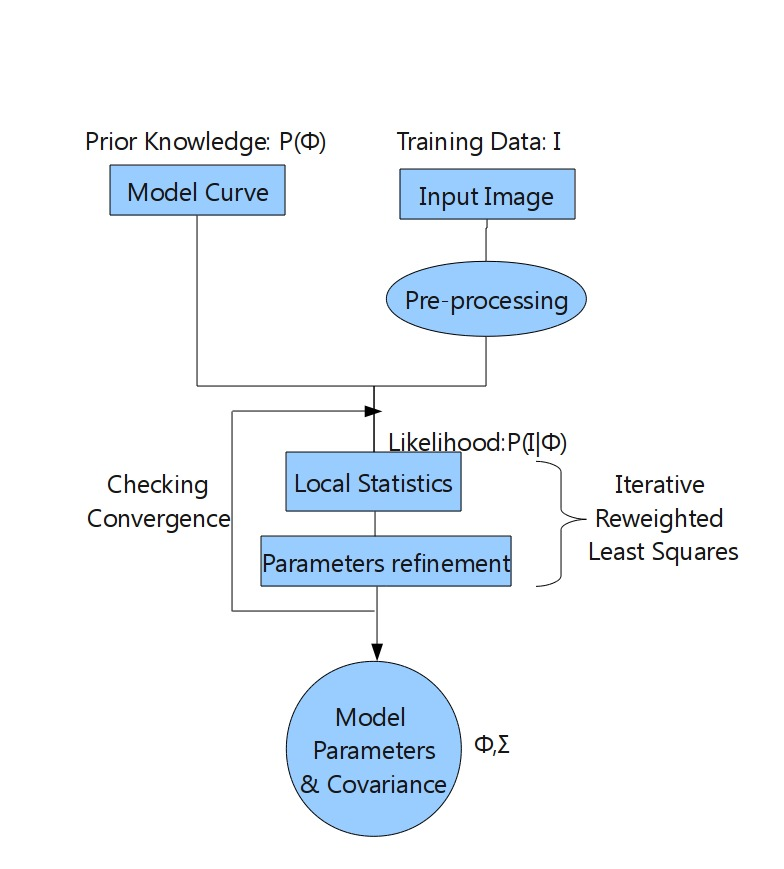
\includegraphics[width=12cm]{images/flowchart.jpg}
  \caption[The flow chart of
  the CCD algorithm]{The flow chart of the CCD algorithm}
  \label{fig:flowchart}
\end{figure}
\begin{enumerate}
\item \textbf{Initialization}: Given an input image as training data, we first choose an initial
contour for an object or feature which will be fitted or tracked, and
some initial values for the means and covariances. In addition, for most practical
applications, 
pre-processing stage is necessary to make the problem easier to solve. 
\item \textbf{Learning of local statistics}: In the step of learning local
  statistics, for each pixel in the
vicinity of the expected curve, two sets of local statistics
are computed, one set for each side of the curve. The local statistics are obtained from
pixels that are close to the pixel on the contour and most likely lie
on the corresponding side of the curve, according to the current
estimate of the model parameters. The resulting local statistics
represent an expectation of "what the two sides of the curve look
like"~\cite{hanek2004contracting}, also known as likelihood.
\item \textbf{Refinement of model parameters}: The conditional distribution, namely
  the product of prior distribution and  the likelihood, is evaluated
  as the cost function. Then MAP estimate is executed to optimize the
  parameters, as a result, MAP value of model parameter vector and
  covariance will be given in this step.
\item \textbf{Checking Convergence}: Check for convergence of either
  the parameters or log cost function. If the convergence criterion is
  not satisfied return to step 2.
\end{enumerate}
Fig.\ref{fig:flowchart} gives the flow chart of the CCD algorithm.

% The CCD algorithm has some interesting similarities to the Expectation-Maximization
% (EM) algorithm (Dempster et al., 1977), which is often used for clustering-based image
% segmentation, a subset of region-based image segmentation (Hermes et al., 2002; Belongie
% et al., 1998). The first step computes local statistics defining an expectation of the pixel
% values (E-step). The second step maximizes this expectation
% (M-step). The CCD algorithm differs mainly by: 1.) using local
% statistics, 2.) exploiting a curve model and optimizing model
% parameters rather than pixel classifications.


\section{Overview of the Thesis}
\label{sec:overview}
The remainder of the work at hand is organized as
follows. Chapter~\ref{chapter:related} describes the related work on
active contour, model-based image segmentation and tracking, as well
as optimization methods. In Chapter~\ref{chapter:SHI}, we give a brief introduction of software
and hardware infrastructure used in the implementation of the CCD
approach. We will focus on the \acronym{OpenCV}{Open Source Computer Vision Library}, \acronym{ROS}{Robot Operating System} and \acronym{PR2}{Personal Robot 2}. Details on shape-space models and parametric
B-Spline curves are discussed in Chapter~\ref{chapter:bspline}, and
Chapter~\ref{chapter:ccd} explains the CCD approach in detail. 
In Chapter~\ref{chapter:experiments}, experiments and results are
demonstrated. In Chapter~\ref{chapter:conclusion}, the work of this
thesis is concluded with the future work for improvement.

%  In
% addition, we evaluate the performance of the CCD algorithm and the CCD
% tracker in terms of robustness, accuracy, and runtime.


                %%% Local Variables: 
%%% mode: latex
%%% TeX-master: "../main"
%%% End: 
\chapter{Related work}
\label{chapter:related}

As mentioned in the previous chapter, the
CCD approach introduced in this chapter is a model-based computer
vision algorithm. The topics of model-based approach in the field of
computer vision have been addressed in numerous research papers.
In this chapter we review selected publications related to the topics
covered in this thesis and try to reveal the revolution process. The
articles have been carefully selected based on the following criteria:
\begin{itemize}
\item Articles on 2-Dimensional and 3-Dimensional deformable models,
  such as snakes and gradient vector flow deformable models\cite{xu2000gradient}.
\item Articles on applying statistical knowledge to the models
\end{itemize}
There are possible overlaps in two categories. We will discuss the
advantages and limitations of these methods related to the work we aim
to solve. In section \ref{2d3ddm} we will discuss the related work
belonging to the first category. This is followed by the introduction
of previous work on statistical models.
% The topics of active contour, the Contracting
% Curve Density approach and model tracking have been addressed in
% numerous research papers.

\section{2-Dimensional and 3-Dimensional deformable model}
\label{sec:2d3ddm}
Many traditional segmentation methods are effected by the assumption that the
images studied in computer vision usually is self-contained, namely,
the information need for a successful segmentation could be extracted
from the images.

In 1980s, a paradigm named \textit{Active Vison}\cite{aloimonos1988active} escape this bind and
push the vision process in a more goal-directed fashion. After that, a
notably successful departure, the \textit{Snake}, is proposed in a
seminar work conducted by Kass. The original paper is
\cite{kass1988snakes}, which spawned many variations
and extensions including the use of Fourier parameterisation\cite{scott1987alternative}, incorporation
of topologically adaptable model\cite{mcinerney1995topologically} and
its application \cite{mcinemey1999topology}, incorporation of discrete
dynamic contour model\cite{lobregt1995discrete}. A realization of snakes
using B-splines was developed in \cite{brigger2000b}. In two
dimensions, The snake has a variation named active shape
model\cite{cootes1995active}, which is a discrete version of this
approach. Gradient Vector Flow\cite{xu1998snakes}, or GVF, is an extension developed
based on new type of external field. Another paper written by the same
authors \cite{xu2000gradient}, concerning convergence properties of
deformable models. In three dimension, a good deal of research works has
been conducted on matching three-dimensional models, both on rigid
\cite{harris1993tracking} and
deformable\cite{terzopoulos1991dynamic}. 

Besides the segmentation,
dynamic models, such as snake and its variations, are greatly used in application of object
tracking. A real-time tracking system based on deformable models, such
as snakes, is developed
in \cite{terzopoulos1992tracking}. It proved that the active shape and
motion estimators are able to deal very effectively with the complex
motions of nonrigid objects. Furthermore, the combination of active
models and Kalman filter theory is also a popular approach to
tracking, some work about this can be found in
\cite{schick1991simultaneous}.

\cite{blake1998active} is a wonderful book about the topics of
geometric and probabilistic models  for shapes and their dynamics.

\section{Statistical models}
\label{sec:sm}
Pattern recognition theory is a general statistical framework which is
important in the study of model-based approaches. This is started from the 1970s
and 1980s when a new interpretation of image was proposed in the
statistical community.  Analyzing the model problems in probabilistic
context has two great advantages. The first is that it approaches the
nature of the problems, the ranges of shapes are defined by a
probability, this provides another viewpoint for curve fitting problem
in the field of computer vision. Another advantage is that after we
convert a problem in pattern recognition, there are abundant tools and
skills to deal with such problem. 
The CCD approach is a method developed in the probabilistic context. 

In \cite{kelemen1999three} and \cite{kelemen1999elastic}, an elegant
use of statistical models for the segmentation of medical images is
designed.  The resulting segmentation system consists of the building
of statistical models and the automatic segmentation of new image data
sets by restricting elastic deformation of models.  The work in
\cite{sclaroff2001deformable} and \cite{liu1999deformable} also
exploit the prior knowledge from the perspective of probability,
furthermore, the statistical shape models enforce the prior
probabilities on objects by designing complicated energy function.  In this thesis, we assume that the shape priors have a Gaussian form in
shape-space. In the case of a norm-squared density over  quadratic spline space,
the prior is a Gaussian Markov Random Field
(MRF)\cite{blake1998active}, which is used widely  for modelling prior
distributions for curves\cite{storvik1994bayesian}.


However, defining a prior distribution for shape is only part of the
problem. Prior knowledge only control the feature interpretation in a
image, a successful segmentation or curve fitting requires to
obtaining the posterior distribution, which takes account of what
shape is actually likely to be present in a particular image. Inspired
by the iterative algorithm k-means\cite{ding2004k} and
Expectation-Maximization (EM)\cite{dempster1977maximum} algorithm, especially the later one, a novel
curve fitting method the ccd algorithms is proposed in
\cite{hanek2004contracting}. Bayesian treatment is used in this
algorithm in incorporation of maximum a posteriori probability (MAP)
\cite{sorenson1980parameter} estimate instead of complicated cost
function. Not like the EM algorithm, the CCD use local statistics
instead of global statistics. Moreover, blurred curve models is
proposed as efficient means for iteratively optimizing. The algorithm
can be used in object localization and object tracking. As an example
of applications of the CCD approach, an efficient, robust and fully
automatic real-time system for 3D object pose tracking in
image sequences is presented in \cite{panin2006fully} and
\cite{panin2006efficient}. Multiocular contracting curve density
algorithm (MOCCD) \cite{hahn2007tracking} is an extension of the CCD
approach. In the paper, it is integrated into tracking system to
tracking human body. 

Both the snake and CCD can be used to build naive tracking
system. However, they are limited by the performance and stability
problems. Several methods achieve a speed-up propagate a Gaussian
distribution of the model parameters over time, such as tracking based
Kalman filter in \cite{brookner1998tracking}. The method is limited by the range of probability
distributions they presented. The condensation algorithm (Conditional
Density Propagation) \cite{isard1998icondensation} is proved to lead
to a marked improvement in tracking performance. Another feature of
this method is that it only consider the pixels on some
perpendiculars. The CCD tracker \cite{hanek2004fitting} uses only
pixels on some perpendiculars like the condensation algorithm, but
focuses on the vicinity of the contour. This means the CCD tracker can
save time and improve performance.

In the CCD algorithm and its variations, the curve fitting probelm is
often converted to an optimization one. The optimization step is
outstanding import for the CCD approach. There are many methods to
deal with optimization, which can be classified into  into two
categories, one is global optimization and another is local
optimization\cite{hanek2004fitting}. The later one is used in the CCD
approach. First, a smoothed objective function is obtained by fitting
the curve model to a large scale description. Then the windows size is
gradually reduced. During the process, many kinds of  numerical
optimization  methods such as  conjugate gradient method , Newton's
method, Gaussian-Newton and Levenberg-Marquardt algorithm
\cite{contourpanin2011} can be used.



                \chapter{Software and Hardware Infrastructure}
\label{chapter:SHI}
In this chapter, we will introduce the software and hardware
infrastructure used in this thesis. In Section~\ref{sec:ros} we introduce the
Robo Operation System. The PR2 robot will be presented in Section
~\ref{sec:pr2}. This is followed by the introduction of OpenCV library.

\section{The Robot Operating System (ROS)}
\label{sec:ros}
% provides libraries and tools to help
% software developers create robot applications. It provides hardware
% abstraction, device drivers, libraries, visualizers, message-passing,
% package management, and more.
ROS is an open-source, meta-operating framework for robot software
development. Ros was originally developed in 2007 by Stanford Artificial Intelligence Laboratory in support of the Stanford AI Robot~\cite{quigley2007stair}. Like an ordinary operating system, it consists of  robot
hardware resources management, low-level device control, implementation
of commonly-used functionality, interprocesses comunication (IPC), and package
management. ROS is based on a pere-to-peer network architecture where
processing takes place in nodes that may receive, post and 
multiplex sensor, control, state, planning, actuator and other
messages. There are several different styles of communication, including synchronous RPC-style communication over services, asynchronous
streaming of data over topics, and storage of data on a Parameter
Server.
Moreover, ROS provides tools and libraries for obtaining, building, writing, and
running code across multiple computers.

ROS is composed of operation system wide library \textbf{ros} and
\textbf{ros-pkg}. The former one is a fundamental library as described
above and the later one is a suit of user contributed packages which
are organized into sets called \textbf{stacks}. The stacks include
many application areas, such as  perception, object identification,
segmentation and recognition, face recognition, motion tracking ,
stereopsis stereo vision, control, planning, grasping and so on. ROS has been ported to many robots and boards.

The goal of ROS is "to support code reuse in robotics research and
development"~\cite{rosintroduction}.  it is designed to enable easily
share and collaborate among developers. Moreover, ROS has many
features, such as compact framework, language independence, easy
testing and scalability.

ROS currently run on on Unix-like operating systems towards which the libary is
geared. Currenty Ubuntu Linux is greatly supported. Moreover, The core
ROS system and its tools and libraries are regularly released as ROS
Distributions~\cite{rosintroduction} under the terms of the BSD license.

\section{PR2}
\label{sec:pr2}
Personal Robot 2 (PR2) is a personal robitics research and development
platform.  It is developed by Willow Garage.  PR2 has two 7-DOF arms and a mobile
base, and its size  is similar to a human. Its sensors system consists of a 5
megapixel camera, a tilting laser range finder, and an inertial
measurement unit. The "texture projector" on PR2 can project a pattern
on the environment to create 3D information captured by the
cameras. PR2 is equiped with 16 CPU cores with 48 Gigabytes of
RAM. Its battery system consists of 16 laptop batteries. PR2 is
controled with ROS system as described in Section~\ref{sec:ros} which
consistes of a series of libraries for perception, navigation and
manipulation.
The experiments of this thesis are partly delivered in PR2 system (Figure~\ref{fig:pr2}).

\begin{figure}[htbp]
  \centering
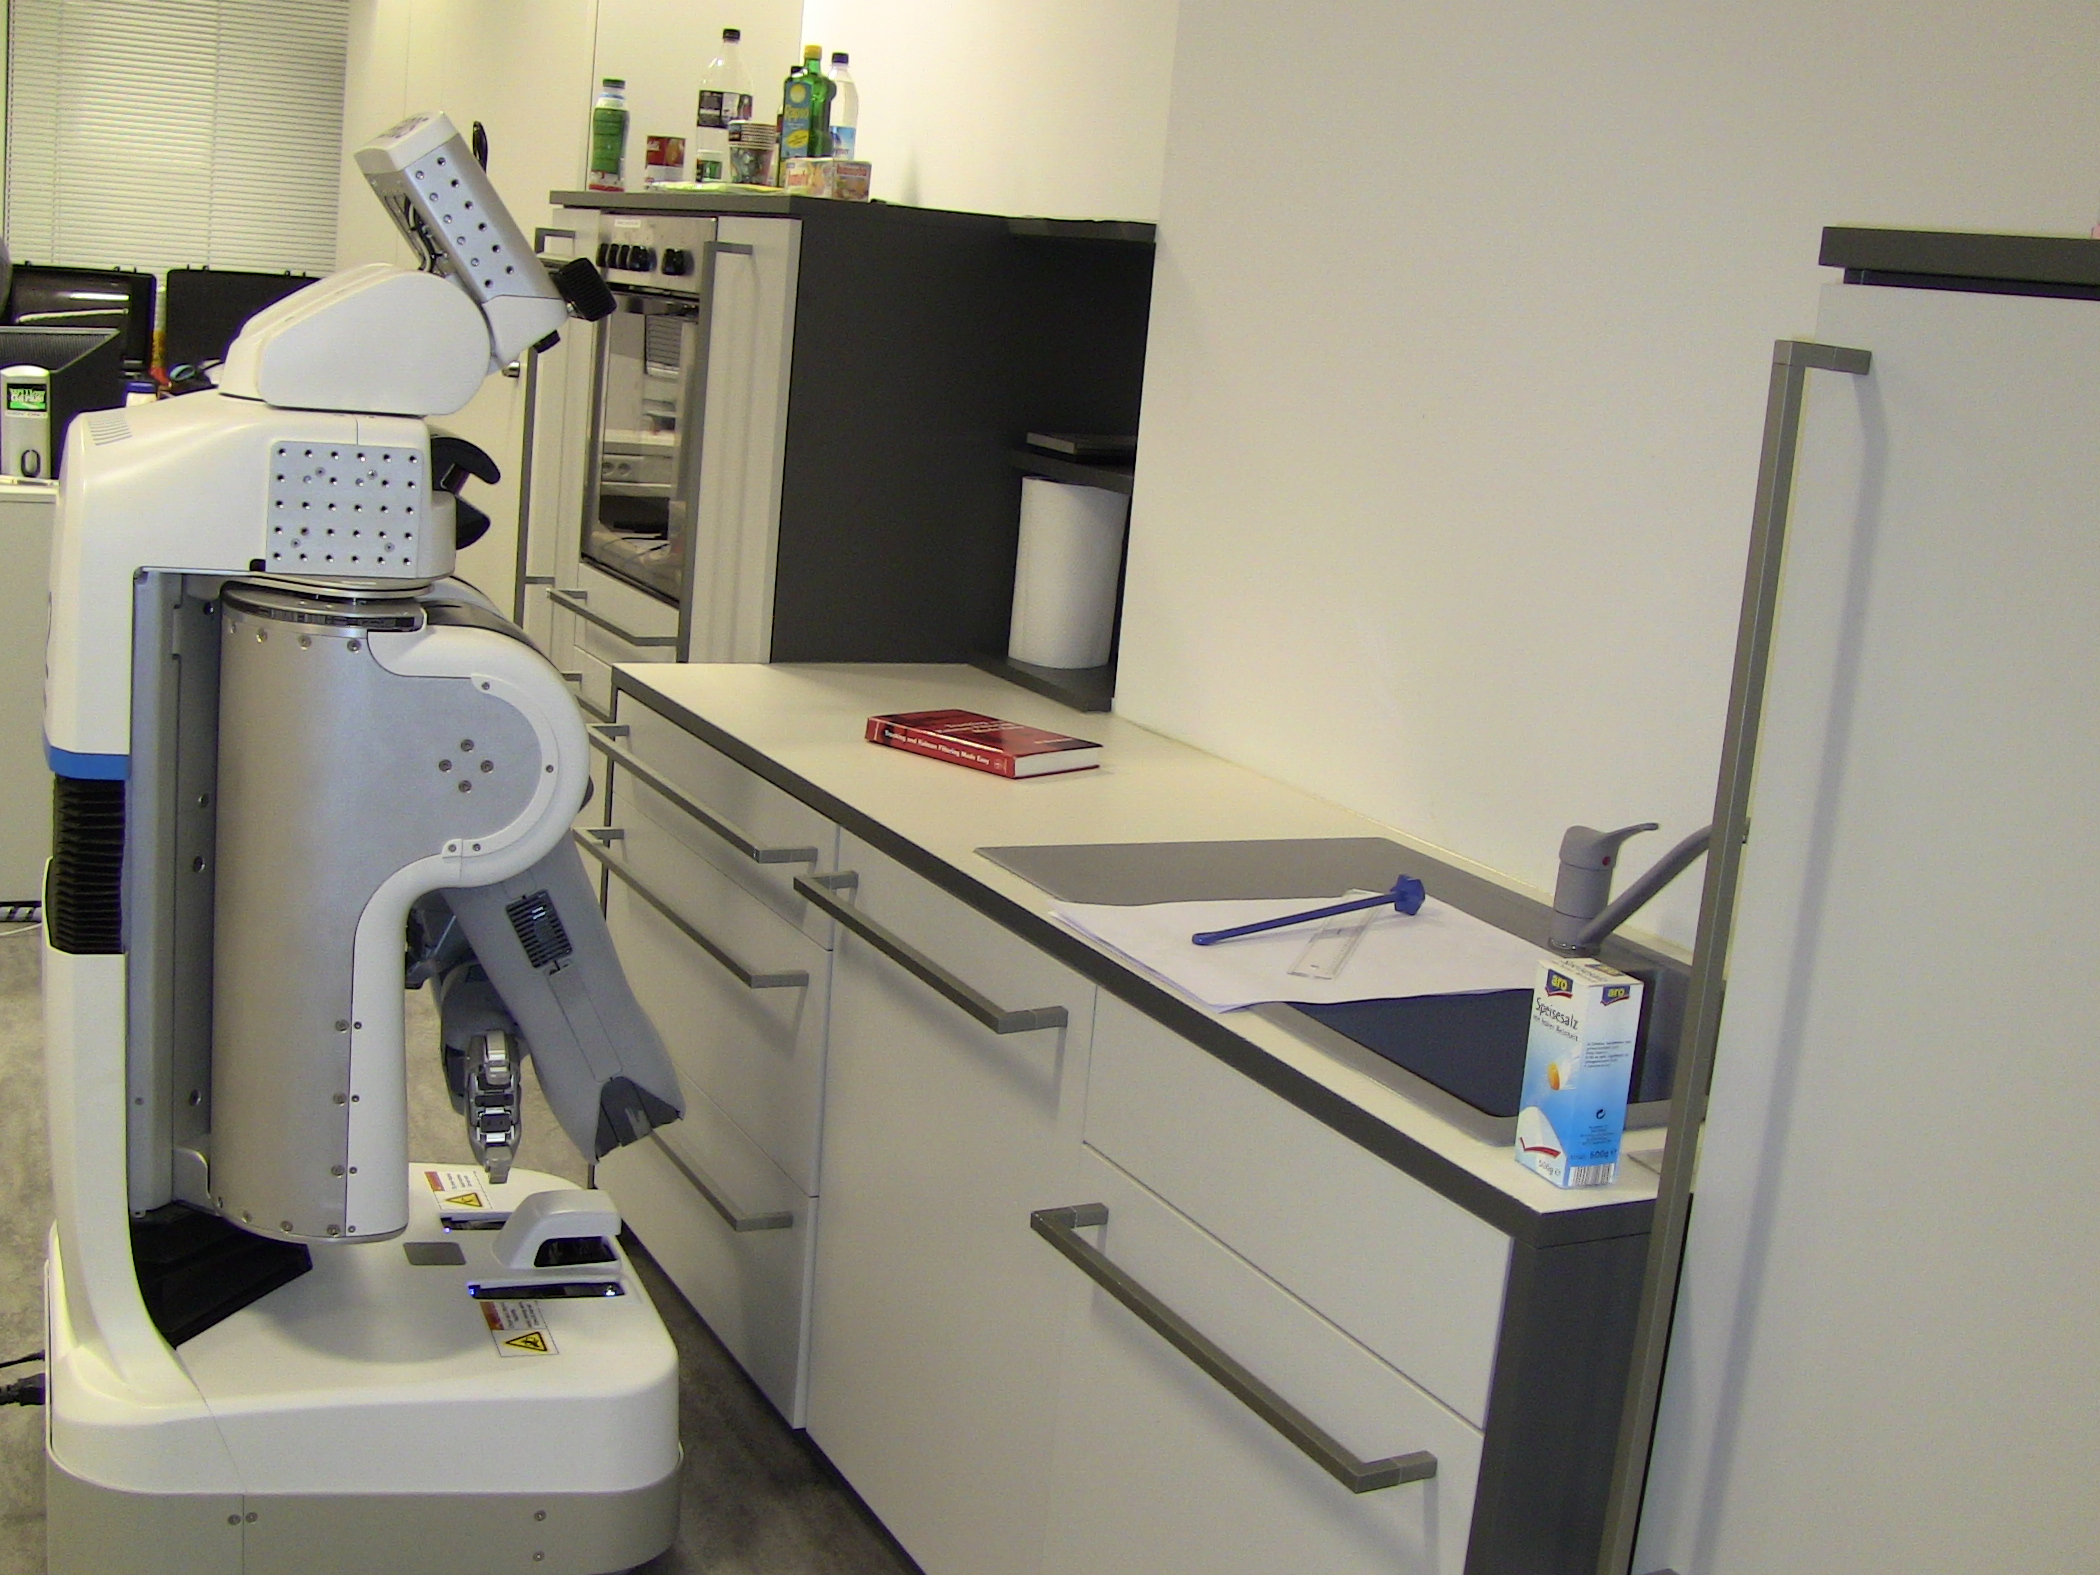
\includegraphics[width=\linewidth]{images/pr2.png}
  \caption[A PR2 robot]{The PR2 robot locate in Cognition for
    Technical Systems (CoTeSys) Lab in Technische Universit\"at M\"unchen.}
  \label{fig:pr2}
\end{figure}

\section{OpenCV Library}
\label{sec:opencv}

OpenCV (Open Source Computer Vision Library) is a library of
programming functions mainly aimed at real time computer vision. It is
originally developed by Intel and now maintained by Willow Garage. It
is free for both academic and commercial usage and released  under the
open source BSD license. The library is cross-platform, which supports
Windows, Linux and MacOX,  in the latest version 2.2, the Android
system is supported.

OpenCV is originally written in C but now full C++ and Python
interfaces are provided. The library is widely used in the field of
computer vision, such as Human-Computer Interaction (HCI); Object
Identification, Segmentation and Recognition; Face Recognition;
Gesture Recognition; Motion Tracking, Ego Motion, Motion
Understanding, Stereo and Multi-Camera
Calibration and Depth Computation, Mobile Robotics (e.g. Android
system).

\begin{figure}[htbp]
  \centering
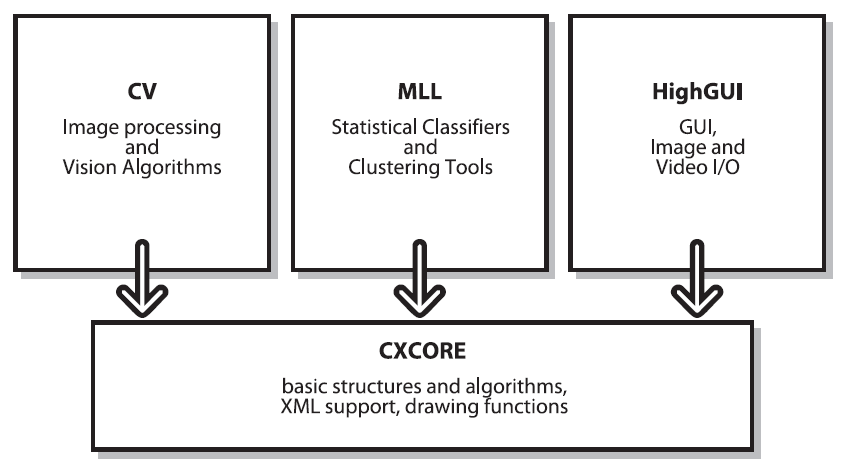
\includegraphics[width=\linewidth]{images/bsopencv.png}
  \caption{The basic structure of OpenCV~\cite{bradski2008learning}}
  \label{fig:bsopencv}
\end{figure}

Currently, OpenCV consists of following five main components~\cite{bradski2008learning}.
\begin{itemize}
\item \textbf{Cv}: image processing and vision algorithms
\item \textbf{MLL}: machine learning library, including statistical classifiers and clustering tools
\item \textbf{HighGUI}: Graphic user interface and Input/Output
  routines for image and video.
\item \textbf{CvCore}: the basic data structures and content
\item \textbf{CvAux}: contains defunct areas (embedded HMM face
  recognition) and experimental algorithms (background/foreground
  segmentation).
\end{itemize}

The B-spline and CCD algorithm in this thesis is implemented using the
OpenCV library.



                \chapter{Shape-space Models and B-spline Curves}
\label{chapter:bspline}
In the CCD algorithm, a parametric curve model is used for
restricting Region of Interest (ROI) and providing prior probability distribution. 
Throughout this thesis, visual contours of observed objects are represented in terms of
parametric spline curves which are widely applied in computer graphics.

In this chapter, we introduce deformable two-dimensional and three-dimensional models called
shape-space models.  In the first section, we start by explaining
spline functions and their construction. Details on how parametric
curves are constructed from spline functions are discussed in the
Section~\ref{sec:pbc}. % This forms the basis for the CCD approach.
\section{B-spline Function}
\label{sec:bsc}
A B-spline is simply a generalisation of a B\'ezier curve, and they possess many
advantages in comparison with B-spline curves~\cite{compgeo}:
\begin{itemize}
\item B-spline curves satisfy all important properties that B\'ezier curves have.
\item B-spline curves provide more control flexibility than B\'ezier
  curves can do. Because the degree of a B-spline curve is separated
  from the number of control points, we can use lower degree curves
  and still maintain a large number of control points.
\item We have a finer shape control because we can change the position
  of a control point without globally changing the shape of
  the whole curve.
\end{itemize} 

In mathematics, every spline function of a given degree,
smoothness, and domain partition, can be represented as a linear
combination of B-splines of that same degree and smoothness, and over
that same partition~\cite{press2007numerical}. In line with this statement, we can
construct  a spline curve parametrized by spline functions that are
expressed as linear combinations of B-splines. 

Given a non-decreasing vector of real values $U = [u_0, \ldots,
u_{m-1}]$ called knot vector, with $u_i$ called the knot, a
B-spline of degree $n$ is parametric curve can be written as follows:
\begin{equation}
  \label{eq:4.1}
  \mathbf{C}(u) =  \sum_{i=0}^{m-n-2} P_{i} B_{i,n}(u) \mbox{ , } u \in [u_{n},u_{m-n-1}]\qquad,
\end{equation}
where $P_i$ are called control points, and $B_{i,n}$ are called
basic functions. For n=0,1,...,m-2, the m-n-1 basis B-splines of degree
n can be defined as:

\begin{eqnarray}
  \label{eq:4.2}
  B_{i,0}(u) &=&  \left\{
\begin{matrix} 
1 & \mathrm{if} \quad u_i \leq u < u_{i+1} \\
0 & \mathrm{otherwise}
\end{matrix}
\right.,\qquad i=0,\ldots, m{-}2 \\
B_{i,n}(u) &=& \frac{u - u_i}{u_{i+n} - u_i} B_{i,n-1}(u) + \frac{u_{i+n+1} - u}{u_{i+n+1} - u_{i+1}} B_{i+1,n-1}(u)
, i=0,\ldots, m{-}n{-}2 \qquad.
\end{eqnarray}

We can write the B-spline compactly in matrix notation as:
\begin{equation}
  \label{eq:4.3}
  \mathbf{C}(u) = 
  \begin{pmatrix}
\mathbf{B}(u)^T & 0 \\
0 &\mathbf{B}(u)^T
  \end{pmatrix}
\mathbf{P}\qquad,
\end{equation}

where vector $\mathbf{P}$ denotes the axis components of control
points:
\begin{equation}
  \label{eq:4.4}
  \mathbf{P} =
  \begin{pmatrix}
    P_x & P_y    
  \end{pmatrix}^T \quad \mathrm{where} \quad P_x =
  \begin{pmatrix}
    P_0^x\\
    \cdots\\
    \cdots\\
    P_{N-1}^x
  \end{pmatrix}\qquad .
\end{equation}
$N$ denotes the number of control points, and $\mathbf{B}(u)$ is a
vector of basis function:
\begin{equation}
  \label{eq:4.5}
  \mathbf{B}(u) = (B_0(u), \ldots, B_{N-1}(u))^T\qquad.
\end{equation}

A example of B-spline curve for different basic functions is depicted
in Fig.~\ref{fig:bspline}. The B-spline is said to be uniform when the knots are equidistant,
otherwise it is non-uniform. In this thesis, we only
consider the uniform case for simplicity.
\begin{figure}[htb]
  \centering
  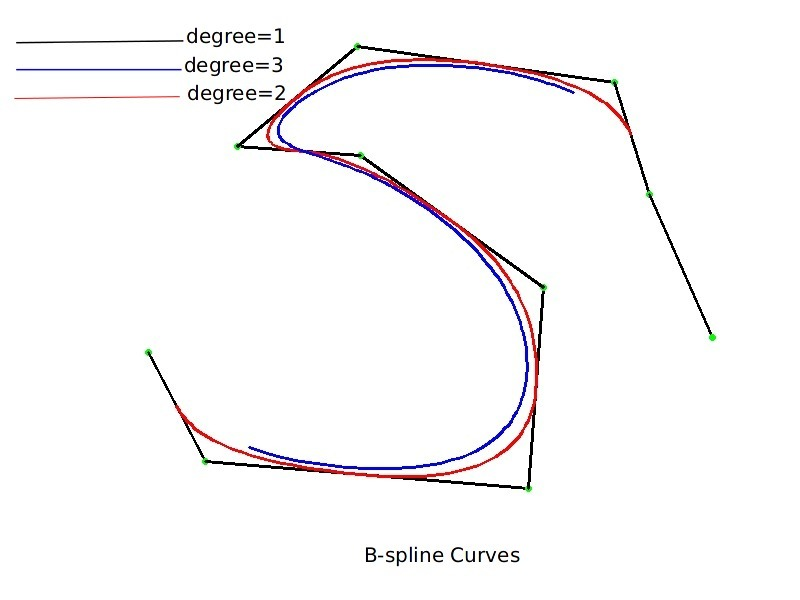
\includegraphics[width=12cm]{images/bspline.jpg}
  \caption[B-spline curves for different
  degrees~\cite{contourpanin2011}]{Black, red, blue curves represent B-splines for degrees 1, 2 and 3 respectively.}
\label{fig:bspline}
\end{figure}

As a special example of the B-spline, we consider the matrix form and
derivative of cubic B-spline which is the most commonly used because
its first and second order derivatives are continuous.

% \subsection{Uniform Quadratic B-spline}
% \label{sec:uqb}

% Because the knot-vector is equidistant, the blending function can
% easily be computed. In each segment, the blending function $\mathbf{b}_{i,2}(u)$ shares the
% same form, as follows:
% \begin{equation}
%   \label{eq:4.3}
%   \mathbf{b}_{i,2}(u) = \begin{cases} \frac{1}{2}u^2 \\ -u^2 + u + \frac{1}{2} \\ \frac{1}{2}(1-u)^2   \end{cases}\qquad ,
% \end{equation}

% With the derivative being: 
% \begin{equation}
%   \label{eq:4.4}
%   \mathbf{b}_{i,2}'(u) = \begin{cases} u \\ -2u + 1 \\ u-1   \end{cases}\qquad .
% \end{equation}

% The matrix-form of uniform quadratic B-spline is then given by:
% \begin{equation}
%   \label{eq:4.5}
% \mathbf{B}_i(u) = \begin{bmatrix} u^2 & u & 1 \end{bmatrix} \frac{1}{2} \begin{bmatrix}
% 1 & -2 & 1 \\
% -2 &  2 & 0 \\
% 1 &  1 & 0 \end{bmatrix}\qquad .
% \end{equation}

\subsection{Uniform Cubic B-spline}
\label{sec:uqb}
Uniform cubic B-spline is the most commonly used form of B-spline, 
the blending function is
\begin{equation}
  \label{eq:4.6}
  \mathbf{b}_{i,3}(u) = \begin{cases} \frac{1}{6}(-u^3+3u^2-3u+1) \\
    \frac{1}{6}(3u^3 -6u^2+4)\\ \frac{1}{6}(-3u^3+3u^2+3u+1) \\
    \frac{1}{6}u^3
   \end{cases}\qquad ,
\end{equation}

with the derivative being: 
\begin{equation}
  \label{eq:4.7}
  \mathbf{b}_{i,3}'(u) = \begin{cases} \frac{1}{2}(-u^2+2u-1) \\
    \frac{1}{2}(3u^2 -4u)\\ \frac{1}{2}(-3u^2+2u+1) \\
    \frac{1}{2}u^2
   \end{cases}\qquad .
\end{equation}


The matrix-form of uniform cubic B-spline is then given by:
\begin{equation}
  \label{eq:4.8}
\mathbf{B}_i(u) = \begin{bmatrix} u^3 & u^2 & u & 1 \end{bmatrix} \frac{1}{6} \begin{bmatrix}
-1 &  3 & -3 & 1 \\
 3 & -6 &  3 & 0 \\
-3 &  0 &  3 & 0 \\
 1 &  4 &  1 & 0 \end{bmatrix}
\begin{bmatrix} \mathbf{p}_{i-1} \\ \mathbf{p}_{i} \\ \mathbf{p}_{i+1}
  \\ \mathbf{p}_{i+2} \end{bmatrix}\qquad .
\end{equation}

\section{Parametric B-spline Curves}
\label{sec:pbc}

In a two-dimensional image, a curve is composed of many discrete points which are
identified by their coordinates. For those points on a curve, their axis
components $x$, $y$ are particular instances of knots value $u$, also known
as splines. Hence, we can define a B-spline curve as:
\begin{equation}
  \label{eq:paramcurve}
  \mathbf{C}(u) = (x(u),y(u))^T = \mathbf{U}(u) \mathbf{P} \qquad ,
\end{equation}
where $\mathbf{U}(u)$ denotes the matrix the mapping control point
vector P to the image
curve $\mathbf{C}(u)$
\begin{equation}
  \label{eq:4.12}
  \mathbf{U}(u) =   \begin{pmatrix}
\mathbf{B}(u)^T & 0 \\
0 &\mathbf{B}(u)^T
  \end{pmatrix}\qquad .
\end{equation}

\subsection{Norm for B-spline curves}
\label{sec:nbc}

Norm and inner product of curves are useful in curve approximation. In
an image plane, using the Euclidean distance measure, we can define the
norm for curves as:
\begin{equation}
  \label{eq:4.13}
  \left| \left| \mathbf{C} \right|\right|^2  = \mathbf{C}^T\mathcal{U}\mathbf{C}\qquad ,
\end{equation}

where $\mathcal{U}$ represents the metric matrix for curves, and can be
defined as 
\begin{equation}
  \label{eq:4.14}
  \mathcal{U} =   \begin{pmatrix}
\mathcal{B}^T & 0 \\
0 &\mathcal{B}^T 
  \end{pmatrix} \qquad .
\end{equation}

$\mathcal{B}$ denotes the metric matrix for a given class of B-spline
function
\begin{equation}
  \label{eq:4.15}
  \mathcal{B}   = \frac{1}{L} \int_0^L \mathbf{B}(u)\mathbf{B}(u)^T \mathrm{d}u\qquad.
\end{equation}

In Fig.~\ref{fig:bsplinenormal}, we use B-spline to generate the contour of a
Cocacola bottle.
\begin{figure}[htb]
  \centering
  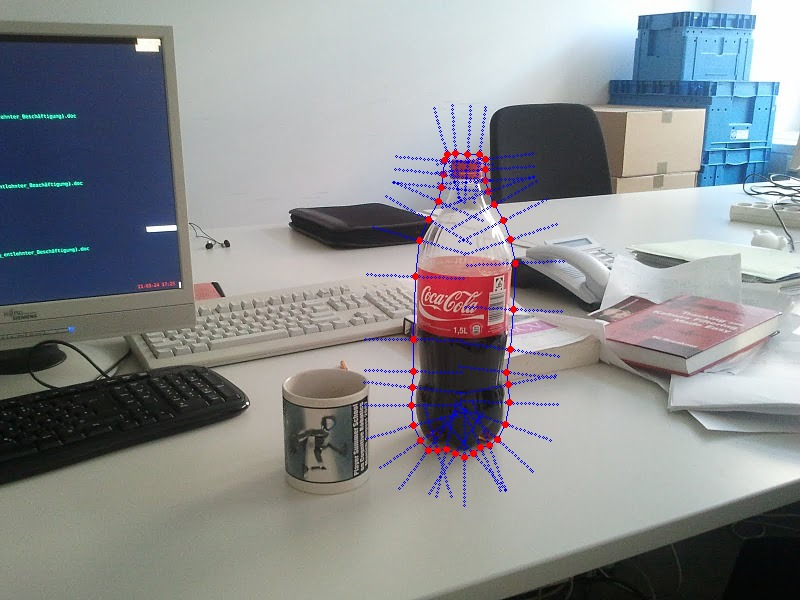
\includegraphics[width=12cm]{images/bsplinenormal.jpg}
  \caption[A contour and its normals]{The contour of a bottle is sketched using a B-spline
    curve, the blue points are pixels in the normal direction.}
\label{fig:bsplinenormal}
\end{figure}


\section{Shape-space models}
\label{sec:ssm}

The shape-space $\mathcal{S}$ is a linear parameterisation of the set of allowed
deformations of a base curve \cite{blake1998active}. Shape-space
$\mathcal{S} = \mathcal{S}(\mathbf{A},\mathbf{P}_0)$ is a linear mapping of a shape-space
vector $\mathbf{\Phi} \in  \mathbb{R}^{N_{\mathbf{\Phi}}}$ to a spline vector $\mathbf{C} \in
\mathbb{R}^{Np}$:
\begin{equation}
  \label{eq:4.16}
  \mathbf{C} = \mathbf{A}\mathbf{X}+ \mathbf{P}_0\qquad,
\end{equation}

where $\mathbf{A}$ is a $N_p \times N_{\mathbf{\Phi}}$ shape-matrix. The
constant  $\mathbf{P}_0$ is a deformable template curve~\cite{blake1998active}. Usually, the
dimension $N_{\mathbf{\Phi}}$ of the shape-space vector is clearly
smaller than the dimension of the spline-vector $N_p$. This makes the
problem more simple and computationally cheaper.

In this chapter, we consider an important shape-space called planar
affine. The planar affine shape-space has 6 DOFs: horizontal
translation, vertical translation, rotation, horizontal scale,
vertical scale and diagonal scale. The planar affine group can be
thought of the class of all linear transformations that can be applied
to a template curve $\mathbf{C}$~\cite{blake1998active}. 

\begin{equation}
  \label{eq:4.17}
  \mathbf{C(u)} = \mathbf{T} + \mathbf{M} \mathbf{C}_0(u)\qquad,
\end{equation}

where $\mathbf{T} = (T_1, T_2)^T$ represents the two-dimensional translation
vector, and $\mathbf{M}$ is a $2 \times 2$ matrix to control the rotation and
scaling, such that $\mathbf{T}$ and $\mathbf{M}$ together can represent the 6 degrees of
freedom of planar affine space. We can write the shape-matrix $\mathbf{A}$
as:
\begin{equation}
  \label{eq:4.18}
  A =
  \begin{bmatrix}
    1 & 0 & P_0^x & 0 & 0 & P_0^y\\
    0 & 1 & 0 & P_0^y & P_0^x & 0
  \end{bmatrix}\qquad. 
\end{equation}

The model parameters $\mathbf{\Phi}$ can be interpreted as:
\begin{equation}
  \label{eq:4.19}
  \mathbf{\Phi} =  (T_1, T_2, M_{11} - 1, M_{22} - 1, M_{21}, M_{12})\qquad.
\end{equation}

The planar affine shape-space discussed above can be extended to
three dimensions, which is more suitable for
non-planar objects. The new space-model needs 8 DOFs to
account for horizontal
translation, vertical translation, rotation, horizontal scale,
vertical scale, diagonal scale and two depth-dependent terms~\cite{blake1998active}. The transformation matrix for the three-dimensional case
can be written as:

\begin{equation}
  \label{eq:4.20}
  A =
  \begin{bmatrix}
    1 & 0 & P_0^x & 0 & 0 & P_0^y & P_0^z & 0\\
    0 & 1 & 0 & P_0^y & P_0^x & 0 & 0 & P_0^z
  \end{bmatrix} \qquad.
\end{equation}

The three-dimensional affine shape-space components have
the following interpretation:
\begin{equation}
  \label{eq:4.19}
  \mathbf{\Phi} =  (T_1, T_2, M_{11} - 1, M_{22} - 1, M_{21}, M_{12},
  \nu_1, \nu_2) \qquad.
\end{equation}
where $\nu_1$, $\nu_2$ are the two additional basis elements.
  
                \chapter{The Contracting Curve Density Algorithm}
\label{chapter:ccd}
In this chapter, we describe the underlying principles of the
Contracting Curve Density algorithm, which is shown to
outperform others in many challenging problems in the field of computer
vision and robotics (\cite{panin2006fully},~\cite{hanek2004contracting},~\cite{hahn2007tracking}). Generally, as mentioned in Section~\ref{sec:sccd},
the algorithm includes three steps: initialization, learning of
local statistics and refinement of model parameters. We describe the
steps in the following sections. 
\section{Pre-processing of Input Images}
\label{sec:init}
% The input of the CCD algorithm is image data (one or multiple images)
% and parametric curve model. Hence, initialization step comprises
% pre-processing of input data and model parametrization.
As Performance of the CCD algorithm depends on the quality of the
input images, we first discuss techniques that alleviate this problem.

Before we start the processing step, it is required to
improve the quality of the images even though the CCD
algorithm is proved robust to noise and clutter in
images. Pre-processing helps solve a CCD problem more easily
because it greatly reduces the variability, and also improves the
extraction of extract features. % Furthermore, pre-processing might be performed in order to
% speed up computation. 
In our case, the data had to be noiseless, shadowless and with sharp edges or boundaries
between objects. There is a group of operations solving this objection.
\begin{itemize}
\item \textbf{Noise reduction}. Many linear and non-linear algorithms
  can help to remove noises, such as mean filter, Gaussian blur,
  Bi-linear interpolation.
\item \textbf{Contrast improvement}. Also we can use a convolution kernel to
  adjust brightness and contrast by selecting a range of input values
  which are mapped to the full output range of intensities.
\item \textbf{Sharpening and detail enhancement}. Scale space is one
  of methods to highlight and enhance fine details in a image.
\end{itemize}

OpenCV provides a series of implementation of these operations. In
this thesis, we filter input images using the OpenCV built-in function
\textit{GaussianBlur}. Note
that for different input data, according to the object properties,
illumination and other physical conditions, different operations
were taken. 

\section{Contour Initialization}
\label{sec:mp}

After the pre-processing of input images,  we initialize the model contour. For the moment, we only consider two-dimensional
affine shape-space consisting of 6 DOFs. % It is followed by the process of
% model parametrization.

In our implementation, we model the
contour as a continuous, differentiable and uniform quadratic or cubic
B-Spline in $\mathbb{R}^2$, which was discussed in Chapter~\ref{chapter:bspline}. 
Given a ROI (region of interest), the first step is to generate
sufficient control points $\mathbf{P} = \{P_0, \ldots, P_{N_p-1}\}$ to
account for the complexity of the object shape (Fig.~\ref{fig:prior}).

\begin{figure}[htb]
  \centering
  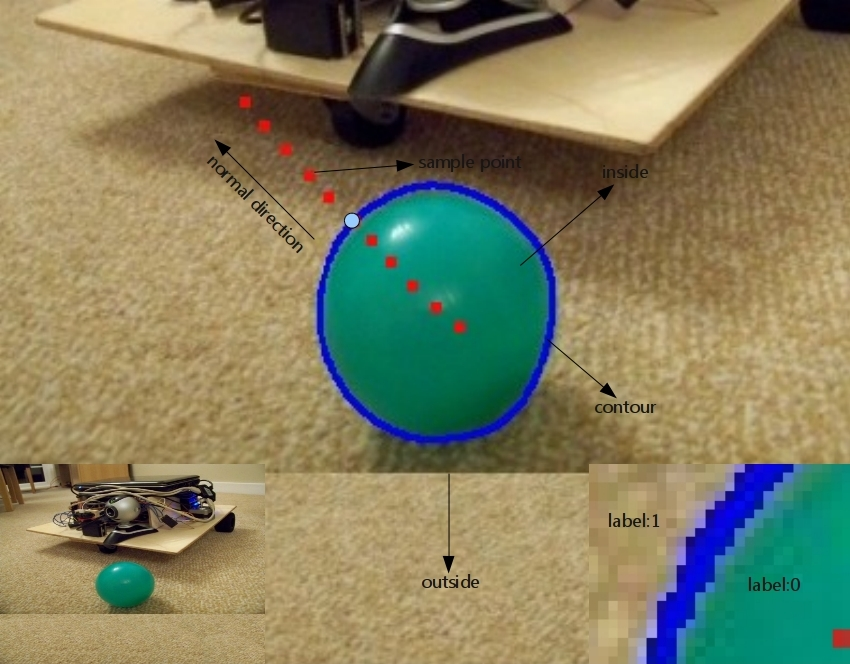
\includegraphics[width=\linewidth]{images/cont.jpg}
\caption[An contour with sample points used for learning local
statistics]{A contour with sample points used for learning local statistics. The blue contour
  divided the image into two parts: outside and inside. As depicted in
  right-bottom image, pixels inside the contour are labeled "0",
  and those outside the contour are labeled "1". For each point on the
  contour (skyblue point), we sample some points (red points) along both positive
  and negative direction.}
\label{fig:prior}
\end{figure}

% Since the former is
% given as a simple form by hand.
% It is easy to use and
% control. However, there are some problems and limitations in case that
% the cost of manual operation is large, or vision deviation due to
% similar brightness between object and background. Therefore,
There are two ways to generate control points:
manual initialization and automated initialization. 
Since the former is rather tedious, two new
intelligent initialization methods are proposed to extract the
contour.
In this thesis, an initial contour estimation method is described and
implemented by employing the well-known SIFT algorithm~\cite{lowe2004distinctive} for
keypoint detection and matching. In Section~\ref{sec:sift_init} it will be discussed in
more detail. In addition, we can convert the point cloud generated
by scanners on PR2 into a polygon. With that polygon we can now model the contour
of an observed object. This method will be described in Section~\ref{sec:tifpc}.

\section{Model Parametrization}
\label{sec:mp}

By applying the (uniform quadratic or cubic) B-spline interpolation to the control points, a new curve
grouped by a sequence of equidistant distributed points is generated
. The B-spline curve is defined in eq.~\ref{eq:paramcurve} and is
composed of a sequence of points $\mathbf{C} = \{C_0, \ldots,
C_{k}\}$, $k = N_{C-1}$. $N_C$ denotes the number of sample points in the
parametric curve. $N_C$ is significant for the
performance of the CCD algorithm, because its value is directly
proportional to the circumference of the observed object. For a high
resolution image, more sample points should be taken into account.
Hence, there is a trade-off between computational expense and the
accuracy. We recommend to compute the circumference of a given object before
determining $N_C$ and sample more points near spinodals and corners to
capture key features of the object.

Since the resulting parametric curve is continuous and
differentiable, we can easily compute the normal vector $\mathbf{n} = \{n_0, \ldots,
n_{k}\}$ and the tangent vector $\mathbf{t} = \{t_0, \ldots, t_{k}\}$,
 which was discussed in Section~\ref{sec:pbc}. 

In the planar affine shape-space $\mathcal{S}$, the contour, a
hypothetical initial estimate, can be compactly represented using a
vector $\mathbf{\Phi}$ with 6 real elements, namely model
parameter vector. From the perspective of probability, the hypothetical
curve gives a uncertainty, the solution of the curving problem is
therefore no longer just a single curve, but a whole family of
possible curves (Fig.~\ref{fig:transform}). The Gaussian probability density for these possible
curves in shape-space $\mathcal{S}$ is given as:

\begin{equation}
  \label{eq:prior}
   p(\mathbf{\Phi}) \propto
\mathrm{exp} \left\{ -\frac{1}{2} (\mathbf{\Phi} -
  \mathbf{m}_{\mathbf{\Phi}})^T \mathbf{\Sigma}_{\mathbf{\Phi}}^{-1} (\mathbf{\Phi} -
  \mathbf{m}_{\mathbf{\Phi}}) \right\}\qquad.
\end{equation}

\begin{figure}[htb]
  \centering
  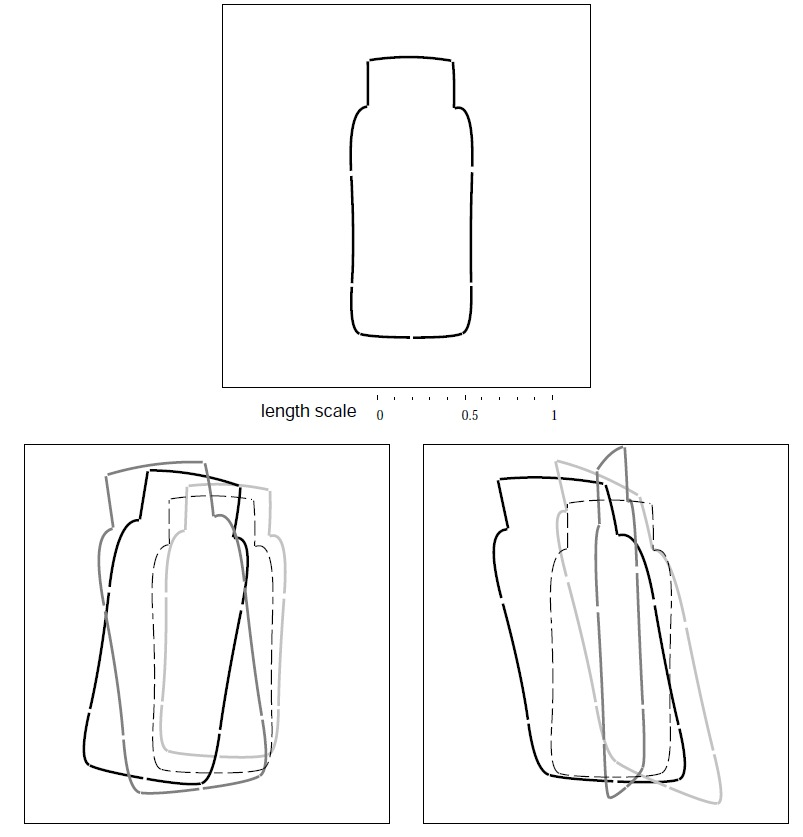
\includegraphics[width=10cm]{images/prior.jpg}
\caption[Sampling from curve families~\cite{blake1998active}]{The top
  figure is the mean shape, the left one represents the euclidean
  similarities, the right one
  sketches some samples in affine space. All these are governed by a
  Gaussian distribution in shape-space with root-mean-square
  displacement of 0.3 length units.}
\label{fig:transform}
\end{figure}

In two dimensions, the current mean model parameter
$\mathbf{m}_{\mathbf{\Phi}}$ is vector with $6$ elements, and current
covariance matrix $\mathbf{\Sigma}_{\mathbf{\Phi}}$ is a $6 \times 6$ matrix, which measures the variability of
how much two groups of model parameters change together. The
information matrix $\mathbf{\Sigma}_{\mathbf{\Phi}}^{-1}$ can be
written as:
\begin{equation}
  \label{eq:infomatrix}
  \mathbf{\Sigma}_{\mathbf{\Phi}}^{-1} = \frac{N_{\mathbf{\Phi}}}{\rho_0^2} \mathbf{A}^T\mathcal{U}\mathbf{A}\qquad,
\end{equation}
where $\rho_0^2$ denotes the mean-square displacement along the entire
curve (\cite{blake1998active}). $\mathbf{A}$ is the shape-matrix, and $\mathcal{U}$ is
metric matrix for curves. $N_{\mathbf{\Phi}}$ represents
the number of model parameters. Note $\rho_0^2$
is a real value and can be computed easily as:
\begin{equation}
  \label{eq:trace}
  \rho_0^2 = \mathrm{tr}(\mathbf{\Sigma}_{\mathbf{\Phi}})\qquad,
\end{equation}
where $\mathrm{tr}(\cdot)$ operation denotes the trace of a matrix.

The pre-processed input images and the parametric curve model have
thus been set up. In the following sections, the iterative procedure of the
CCD algorithm will be described in detail.

\section{Local Statistics}
\label{sec:ls}

\subsection{Collecting Local Information}
\label{sec:cls}

As claimed in Chapter~\ref{sec:ccdcfp}, one of advantages of the
model-based approach is that we can restrict a task at hand to the ROI
which is
expected to reduce the computational cost. Hence, we first define
the region which contains pixels in the vicinity of the expected image
curve. Considering the complexity and the expense of computing, it is practicable
to choose those pixels that are actually required for interpolation along
normals of the curve (Fig.~\ref{fig:prior}). This is proved useful and important for image
perception and real-time tracking system. In the implementation of
this thesis, the processing is limited to a segment of each normal within
a search region. A fixed distance $h$ along the normal segment is
chosen according to the hypothetical uncertainty of the parametric curve. In the
special case of the norm-squared prior in spline space, a reasonable
search segment is determined as follows:

\begin{equation}
  \label{eq:radius}
  h = \sqrt{2} \rho_0 = \sqrt{\mathrm{tr}(\mathbf{\Sigma}_{\mathbf{\Phi}}\mathbf{A}^T\mathcal{U}\mathbf{A})}\qquad.
\end{equation}

$h$ denotes the size of a \textit{window} which is used for computing
the local statistics. In the beginning of the iterative procedure, the value
is relatively big and only roughly approximates the vicinity of the image curve
. The
uncertainty is reduced after further iteration steps and as a result, the $h$ becomes smaller and
smaller. After determining the length of the search segment, 
a set of points located on these segments can be collected and
evaluated. Note that the parametric model curve is not required to be
closed, but it shall always encompass a limited area. We only plan to
analyze the pixels located in the vicinity of the contour (red sample
pixels in Fig.~\ref{fig:prior}). Therefore,
we should pay attention to limit the search distance on the
\textit{inner} side in order to avoid crossing the opposite
boundary to sample pixels from the wrong area~\cite{panin2006fully}. In order to
decrease the computational expense, it is advisable to uniformly sample those
pixels on both segments in the vicinity of the contour. On the other
hand, we should avoid to collect too small number of pixels, because
it is statistically invalid and can not
capture all features (e.g. spinodals and corners) of the contour. Let us denote the
sample distance using $\Delta h$, then the overall number of spaced
sample points $L$ ($2L$ for both sides in all) can be given by:
\begin{equation}
  \label{eq:sample}
  L = \lfloor \frac{h}{\Delta h} \rfloor\qquad.
\end{equation}

Note that the goal of the algorithm is to assign each pixel
($\mathrm{v}_{k,l}, k \in [0,\ldots,N_{\mathrm{C}}-1], l \in [0,
2L-1]$) on either side of the contour. By doing so we thus run into a
classification problem.
Although each pixel should be assigned to one and only
one class so that the target variable is discrete, we can model the
posterior probabilities that lie in $(0,1)$ interval, which converts the classification into the regression problem. To achieve the latter, we model the probabilistic
assignments $\mathbf{a}_{v}$ for each pixel $\mathrm{v}_{k,l}$ as following:
\begin{equation}
  \label{eq:pa}
  \mathbf{a}_v  = (a_{v,1}, a_{v,2})^T\qquad,
\end{equation}
where $a_{v,1}$ describes to which extent a pixel $v$ is expected to
be influenced by side $1$ of the curve, and $a_{v,2}$ is equivalent
for side 2 given by $a_{v,2} = 1- a_{v,1}$. For arbitrary curve
$\mathbf{C}$, it is difficult to give a closed form of $a_v$. In the
following, an efficient approximation of the assignment is derived.

We will first evaluate the \textbf{signed} distance $d_{k,l}$ between pixel
$\mathrm{v}_{k,l}$ and a given curve $\mathbf{C}$
(Fig.~\ref{fig:dis}), which
can be approximated by:
\begin{equation}
  \label{eq:dis}
  d_{k,l} = \mathbf{n}_k \cdot ( \mathbf{v}_{k,l} - C_k)\qquad,
\end{equation}

\begin{figure}[htbp]
  \centering
  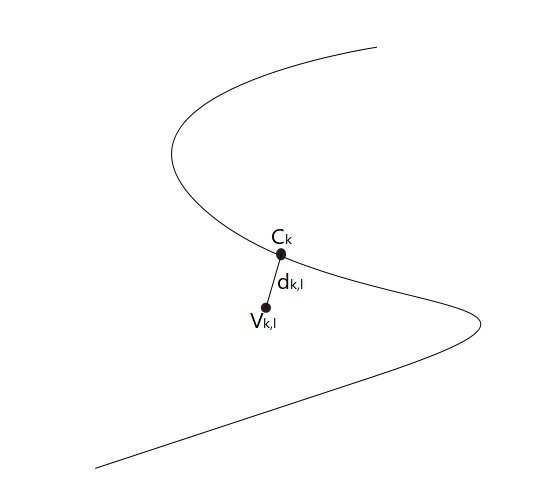
\includegraphics[width=10cm]{images/dis.jpg}
  \caption[The distance between a curve point and a pixel in the vicinity
  of a contour]{The distance between a curve point and a pixel in the
    vicinity of a contour: $C_k$ is the curve point, $v_{k,l}$ is a
    pixel in the perpendicular of the contour, $d_{k,l}$ is the
    distance between $C_k$ and $v_{k,l}$.}
  \label{fig:dis}
\end{figure}

where $\mathbf{v}_{k,l} = {x_{k,l} \choose y_{k,l}}$ is the axis
components of a pixel
$\mathrm{v}_{k,l}$, and $C_k$ is the equivalent for point $C$ on the
curve given by ${x_k \choose y_k}$. Now consider that the curve is
distorted by a Gaussian $p(\mathbf{\Phi})$ which makes the displacement $d_{k,l}$ also Gaussian distributed: $p(d_{k,l}) \sim
\mathcal{N}(d_{k,l}|m_d, \sigma)$, where $m_d$ and $\sigma$ are mean
and covariance of the distribution. Covariance $\sigma$ is expressed as:
\begin{equation}
  \label{eq:cov}
  \sigma = \mathbf{n}_k \cdot \mathbf{J}_k \cdot \mathbf{\Sigma}_{\Phi}
  \cdot \mathbf{J}_k^T \cdot \mathbf{n}_k^T\qquad,
\end{equation}
where $\mathbf{J}_k$ is the Jacobian of curve $\mathbf{C}$. $\sigma$
can be taken as the uncertainty of the curve along the normal
introduced by the covariance
$\mathbf{\Sigma}_{\mathbf{\Phi}}$, it is a constant and can be
evaluated offline. The variable
$\frac{d_{k,l}}{\sigma}$ now becomes a linear function with respect to $\mathbf{\Phi}$.

In order to apply the probabilistic generative models to the
classification problem,
% calculate the the probability that a point lies on side 1 of the curve
we need to transform the linear function of $\mathbf{\Phi}$ using a
non-linear activation function $f(\cdot)$~\cite{bishop2006pattern}:
\begin{equation}
  \label{eq:nonla}
  a_{v,1} = f(\frac{d_{k,l}}{\sigma})\qquad.
\end{equation}
Currently, two main non-linear activation functions are mostly used
to solve the classification problem. The first is known as the
\textit{logistic sigmoid} function, and is given by:
\begin{equation}
  \label{eq:logistic}
  a_{v,1} =
  \frac{1}{1+\mathrm{exp}(\frac{d_{k,l}}{\sqrt{2}\sigma}))}\qquad .
\end{equation}
The term \textit{sigmoid} stands for
S-shaped~\cite{bishop2006pattern}. In~\cite{hanek2004contracting},
another activation function named probit is used, which is defined by:
\begin{equation}
  \label{eq:erf}
  a_{v,1} = \frac{1}{2}erf(\frac{d_{k,l}}{\sqrt{2}\sigma} + 1)\qquad ,
\end{equation}
where the error function of a Gaussian distribution is used. Both
two functions in Eq.~\ref{eq:erf} and Eq.~\ref{eq:logistic} are
S-shaped (Fig.~\ref{fig:s-shaped}).
\begin{figure} 
  \begin{minipage}[t]{0.5\linewidth} 
    \centering 
        \subfloat[logistic sigmoid function]{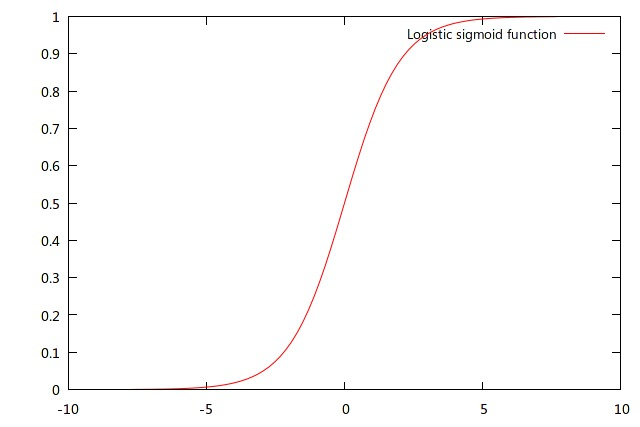
\includegraphics[width=8.0cm]{images/logistic.jpg}}
  \end{minipage}% 
  \begin{minipage}[t]{0.5\linewidth} 
    \centering 
    \subfloat[error function]{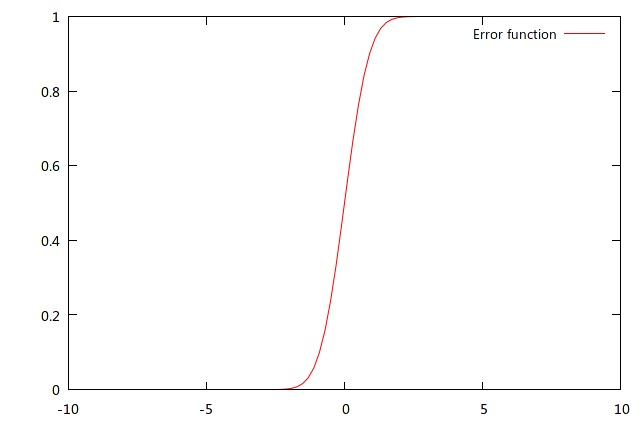
\includegraphics[width=8.0cm]{images/erf.jpg}}
  \end{minipage} 
\caption[Logistic sigmoid function and probit function]{Logistic
  sigmoid function and probit function: Both functions
  are S-shaped}
\label{fig:s-shaped}
\end{figure}

In this thesis, we use both of them to implement the algorithm. They give
similar results but have different behaviors. Logistic sigmoid function
can be perfectly interpreted from the perspective of
probability. Consider the side $s \in \{0,1\}$, the posterior
distribution for side $s = 1$ can be written as:
\begin{eqnarray}
  \label{eq:pdfs}
  p(s=1|I) &=& \frac{p(I|s=1)p(s=1)}{p(I|s=1)p(s=1)
    + p(I|s=2)p(s=2)}\\
&=&  \frac{1}{1+exp(-\mathcal{R})}\qquad,
\end{eqnarray}
where I is pixels' RGB value, and $\mathcal{R}$ is defined as:
\begin{equation}
  \label{eq:ratio}
  \mathcal{R} = \frac{p(I|s=1)p(s=1)}{p(I|s=2)p(s=2)}\qquad.
\end{equation}
The logistic sigmoid plays an important role in many classification
algorithms. It satisfies the symmetry property, and its inverse 
is known as \textit{logit} function, which represents the log of the
ratio of probabilities $ln [p(s=1|I)/p(s=2|I)]$ for the two classes,
also known as the log odds~\cite{bishop2006pattern}.

The logistic sigmoid function can be used to transform a broad range
of class-conditional distributions, described by the exponential
family, to a non-linear posterior class probabilities. Since not all choices of
class-conditional density are trivial, the probit function is explored
to cope with other complex distributions. The results of logistic
sigmoid function and probit function tend to be similar, except that the
probit function is sensitive to outliers because the logistic sigmoid
decays asymptotically like $\mathrm{exp}(-x)$ for $x \rightarrow \infty$, whereas
for the probit activation function the decay is like $\mathrm{exp}(-x^2)$.

% Generally, we can call this approximation process as \textit{fuzzy} (or \textit{smooth})
% assignment. The accuracy of this assignment will increase as the
% uncertainty of curve governed by covariance $\mathbf{\Sigma}_{\mathrm{\Phi}}$ decreases.

With this assignment and following the suggested rule in~\cite{hanek2004contracting}, we now start to assign two suitable weighting functions
$\omega_1$, $\omega_2$ to the pixels $\mathrm{v}_{k,l}$ along the
normal for the two sides of the curve. the weighting functions are
defined as:

\begin{equation}
  \label{eq:weight}
  \omega_{1/2}(d_{k,l}) = C\left(\frac{a_{1/2}(d_{k,l}) -
    \gamma_1}{1-\gamma_2}\right)^4 \left[e^{-d_{k,l}/(2\hat{\sigma}^2)} - e^{-\gamma_2}\right]^+\qquad,
\end{equation}
where $\gamma_1$ equals to $0.5$ (disjoint weight assignment) and $\gamma_2$
equals to $4$ for the truncated Gaussian~\cite{hanek2004contracting}. 

\begin{figure} 
  \begin{minipage}[t]{0.45\linewidth} 
    \centering 
        \subfloat[]{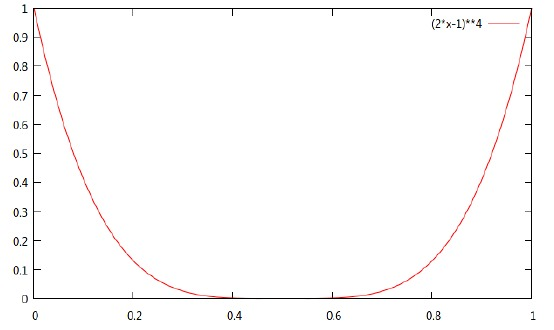
\includegraphics[width=2.0in]{images/weight1.jpg}}
  \end{minipage}% 
  \begin{minipage}[t]{0.45\linewidth} 
    \centering 
    \subfloat[]{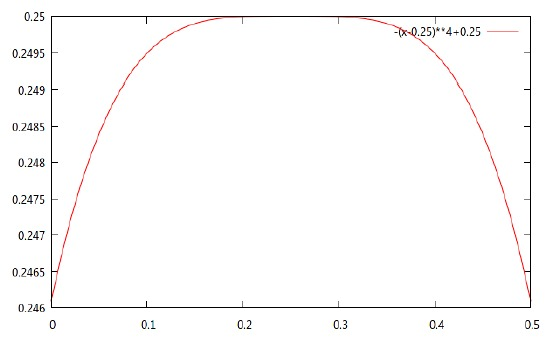
\includegraphics[width=2.0in]{images/weight2.jpg}}
  \end{minipage} 
\caption[Weight functions]{The weight functions of the two sides of the contour, a) the
  weight function along the positive direction (outside) in the normal of the
  contour. b) the weight function along the negative direction (inside). }
\label{fig:weight}
\end{figure}

In addition, the standard
deviation is chosen in order to cover the specified distance $h$,
which yields 
\begin{equation}
  \label{eq:deviation}
  \hat{\sigma} = \max \left[\frac{h}{\sqrt(2\gamma_2)}, \gamma_4
  \right], \sigma  = \frac{1}{\gamma_3} \hat{\sigma}\qquad,
\end{equation}

with the two additional constants $\gamma_3 = 6$ (linear dependence
between $\sigma$ and $\hat{\sigma}$) and $\gamma_4 = 4$ (minimum
weighting window width) as discussed in~\cite{panin2006efficient}. 

In the implementation of this thesis,
there are $2 \cdot L \cdot N_C$ distances, fuzzy assignments
and weight functions which leads to as many weight functions being evaluated offline and stored in an array. Now we have restricted our analysis region of interest in the
limited area, and collected all statistical information required to learn
local statistics. In the next part, we will evaluate the local
statistics.

\subsection{Learning Local Statistics}
\label{sec:lls}

Given the pixel coordinates and RGB values (For the moment, we only consider raw RGB
statistics), assignment and weight
function, local mean vectors $\mathbf{m}_{v,s}$  and local covariance matrix
$\mathbf{\Sigma}_{\mathbf{\Phi}}$ will be derived for each side $s \in
\{1,2\}$ of the curve.
We first calculate the zero, first and second order weighted moments:
\begin{eqnarray}
  \label{eq:localm}
  M_{k,s}^{(0)}(d_{k,l,s}) &=& \sum_{l=0}^{2L-1} \omega_s(d_{k,l})\\
  \mathbf{M}_{k,s}^{(1)}(d_{k,l,s}) &=& \sum_{l=0}^{2L-1} \omega_s(d_{k,l}) \mathrm{I}_{k,l}\\
  \mathbf{M}_{k,s}^{(2)}(d_{k,l,s}) &=& \sum_{l=0}^{2L-1} \omega_s(d_{k,l}) \mathrm{I}_{k,l}\mathrm{I}_{k,l}^T\qquad,
\end{eqnarray}

where $\mathbf{I}$ is just the raw RGB value of a pixel, for a
3-channel image and the values of three components
are  between 0 and 255. The local mean vectors $\mathbf{m}_{v,s}$  and
the local covariance matrices
$\mathbf{\Sigma}_{\mathbf{\Phi}}$  are obtained by:
\begin{eqnarray}
  \label{eq:localmean}
  \mathbf{m}_{k,s} &=& \frac{\mathbf{M}^{(1)}_{k,s}}{M^{(0)}_{k,s}}\\
  \label{eq:localcov}
  \mathbf{\Sigma}_{k,s} &=& \frac{\mathbf{M}^{(2)}_{k,s}}{M^{(0)}_{k,s}}
  - \mathbf{m}_{k,s}\mathbf{m}_{k,s}^T  + \kappa \mathbf{I}\qquad.
\end{eqnarray}
In Eq.~\ref{eq:localcov}, $\kappa I$  means an identity matrix scaled by
$\kappa$ in order to avoid numerical singularity.Later it is namely
required to calculate the inverse matrix of
$\mathbf{\Sigma}_{k,s}$. In our experiments, we choose $\kappa$ to be
$\kappa = 0.5$, which is efficient to avoid numerical problems in the
process of iteration.

With the local mean vectors $\mathbf{m}_{v,s}$  and the local covariance matrices
$\mathbf{\Sigma}_{\mathbf{\Phi}}$, we can compute the
likelihood function   $p(\mathbf{I}_{k,l} | \mathbf{m}_{v,1}, \mathbf{m}_{v,2},
  \mathbf{\Sigma}_{v,1}, \mathbf{\Sigma}_{v,1})$ for each pixel
  $\mathrm{v}_{k,l}$. In terms of observation model, the likelihood
  function describes how probable the observed data set is for
  different settings of the parameter vector. Hence, we first establish
  the relation between image data $\mathrm{I_{k,l}}$ and the model
  parameter $\mathbf{\Phi}$. Here we model the pixel value
  $\hat{\mathbf{m}}_{k,l}$ and $\hat{\mathbf{\Sigma}}_{k,l}$
  for all pixels $\mathrm{v_{k,l}}$ in the vicinity of the curve as the
  linear combination of $\mathbf{m}_{v,1}$ and $\mathbf{m}_{v,2}$:
  \begin{equation}
    \label{eq:meankl}
    \hat{\mathbf{m}}_{k,l} = a_{v,1}(d_{k,l})\mathbf{m}_{v,1} + a_{v,2}(d_{k,l})\mathbf{m}_{v,2}\qquad.
  \end{equation}

If we define  $\hat{\mathbf{\Sigma}}_{k,l}$ using the rule as
$\hat{\mathbf{m}}_{k,l}$ resulting in a function with respect to $d_{k,l}$, the computational cost in the procedure of
parameters refinement which is discussed in the next section  will be very high. Instead, we decide to
model the covariance matrix $\hat{\mathbf{\Sigma}}_{k,l}$ following the
rule in~\cite{hanek2004fitting}, but we discard this relation:
\begin{equation}
  \label{eq:sigmakl}
  \hat{\mathbf{\mathbf{\Sigma}}}_{k,l} = a_{v,1}(d_{k,l})\mathbf{\Sigma}_{v,1} + a_{v,2}(d_{k,l})\mathbf{\Sigma}_{v,2}\qquad.
\end{equation}

Now for each observed pixel $\mathbf{I}_{k,l}$, the likelihood
function is given by:
\begin{equation}
  \label{eq:likelihood}
p(\mathbf{I}_{k,l} | \mathbf{m}_{v,1}, \mathbf{m}_{v,2},
  \mathbf{\Sigma}_{v,1}, \mathbf{\Sigma}_{v,1}) = p(\mathbf{I}_{k,l} | \hat{\mathbf{\mathbf{m}}}_{k,l},\hat{\mathbf{\mathbf{\Sigma}}}_{k,l}) \qquad.
\end{equation}
However, we require the likelihood for all pixels in the vicinity of
the curve. If we consider the coupling or other complex relation among
different group of pixels, the problem will become intractable and the cost of computing will be very expensive. We can
avoid these problems if we assume pixels to be drawn independently from the same distribution
, namely independent and identically distributed
(i.i.d)~\cite{bishop2006pattern}. Thus we can model the likelihood function as:
\begin{equation}
  \label{eq:liklihoodall}
  p(\mathbf{I}_{\mathcal{V}} |
  \hat{\mathbf{\mathbf{m}}}_{\mathcal{V}},\hat{\mathbf{\mathbf{\Sigma}}}_{\mathcal{V}})
  = \prod_l \prod_k p(\mathbf{I}_{k,l} | \hat{\mathbf{\mathbf{m}}}_{k,l},\hat{\mathbf{\mathbf{\Sigma}}}_{k,l}) \qquad.
\end{equation}

The index $\mathcal{V}$ indicates quantities for all pixels $v$ in
$\mathcal{V}$. Note that we only take into account those pixels which are
in the vicinity $\mathcal{V}$ of the curve, whereas pixels outside
$\mathcal{V}$ are not considered.

Having the likelihood function of observed pixels, as well as
the input data and prior knowledge, now we can go into the parameters
refinement stage to model the conditional distribution.

\section{Refinement of  Parameters}
\label{sec:ref}
In this section, an iterative reweighted least square (IRLS) process
is executed to refine parameters, model parameter vector and covariance matrix.

With the likelihood function in Eq.~\ref{eq:liklihoodall} and prior distribution in
Eq.~\ref{eq:prior}, we can model the conditional possibility distribution using:
 % we can estimate the $\hat{\Phi}$ using MAP which is based the
% Bayesian treatment.
% Firstly, the posterior distribution holds
\begin{align}
\label{eq:costf}
    p(\mathbf{\Phi}|\mathbf{\mathbf{I}}_{\mathcal{V}}) 
    \propto &
    p(\mathbf{\mathbf{I}_{\mathcal{V}}}
    |\hat{\mathbf{\mathbf{m}}}_{\mathcal{V}}(\mathrm{\Phi}),\hat{\mathbf{\mathbf{\Sigma}}}_{\mathcal{V}}(\mathrm{\Phi}))p(\mathbf{\Phi}
    | \mathbf{m}_{\mathbf{\Phi}},
    \mathbf{\mathbf{\Sigma}}_{\mathbf{\Phi}})\nonumber\\
    = & {\frac{1}{{(2\pi)}^{1/2}}}
      \frac{1}{|\mathbf{\Sigma}_{\mathbf{\Phi}}|}
      \mathrm{exp}\{-\frac{1}{2}{(\phi-m_{\mathbf{\Phi}})^T{\mathbf{\Sigma}_{\mathbf{\Phi}}}^{-1}(\phi-\mathbf{m}_{\mathbf{\Phi}})}\}\cdot
    \nonumber\\ 
    & \prod_{k = 0}^{N_{C}-1} \prod_{l=0}^{2L-1}{\frac{1}{(2\pi)^{1/2}}
        \frac{1}{|\hat{\mathbf{\Sigma}}_{k,l}|} \mathrm{exp}\{-\frac{1}{2}
        {\left[I_{k,l}-\hat{\mathbf{m}}_{k,l}(a_{v,1})\right]^T\hat{\mathbf{\Sigma}}_{k,l}^{-1}\left[I_{k,l}-\hat{\mathbf{m}}_{k,l}(a_{v,1})\right]}
      }\}\qquad.
\end{align}
The difference between this conditional distribution and posterior
distribution is that here the former function has not been normalized yet.
If applying logarithm operation to the conditional possibility
distribution, we can define a common cost function $\mathcal{Q}$,
which is given by:
\begin{align}
  \label{eq:costd}
  \mathcal{Q} = & -2 \ln \left\{  p(\mathbf{\mathbf{I}_{\mathcal{V}}}
    |\hat{\mathbf{\mathbf{m}}}_{\mathcal{V}}(\mathrm{\Phi}),\hat{\mathbf{\mathbf{\Sigma}}}_{\mathcal{V}}(\mathrm{\Phi}))p(\mathbf{\Phi}
    | \mathbf{m}_{\mathbf{\Phi}},
    \mathbf{\mathbf{\Sigma}}_{\mathbf{\Phi}})\right\}\nonumber\\
 = & \ln{(2\pi)} + 2\ln{|\mathbf{\Sigma}_{\mathbf{\Phi}}|} +
 {\mathbf{\Phi}}^T{\mathbf{\Sigma}_{\mathbf{\Phi}}}^{-1}\mathbf{\Phi}
 + 2LN_{C} \cdot \ln{2\pi} + \nonumber \\
& 2\sum_{k = 0}^{N_{C}-1} \sum_{l=0}^{2L-1}{\ln{|\mathbf{\Sigma}_{k,l}|}} + \sum_{k = 0}^{N_{C}-1} \sum_{l=0}^{2L-1}
\left\{{\left[I_{k,l}-\hat{\mathbf{m}}_{k,l}(a_{v,1})\right]^T\hat{\mathbf{\Sigma}}_{k,l}^{-1}\left[I_{k,l}-\hat{\mathbf{m}}_{k,l}(a_{v,1})\right]}\right\}\qquad.
\end{align}

We interpret the estimate $\hat{\mathbf{\Phi}}$ of the model
parameters $\mathbf{\Phi}$ as  the mean $\mathbf{m}_{\mathbf{\Phi}}$ of a Gaussian
approximation of the posterior distribution, and
$\hat{\mathbf{\Phi}}$ can be evaluated as:
\begin{equation}
  \label{eq:maxcost}
  \hat{\mathbf{\Phi}} =
  \mathbf{m}_{\mathbf{\Phi}}\underset{\mathbf{\Phi}}{\arg\max} \
  (\mathcal{Q}) \qquad.
\end{equation}

To optimize $\mathcal{Q}$ based on the estimated $m_{\mathbf{\Phi}}$,
the approximation to the Hessian matrix can be adopted. First we
compute the partial derivatives of $\mathcal{Q}$:

\begin{equation}
\label{eq:partcost}
\nabla_{\mathbf{\Phi}}\{{\mathcal{Q}(\mathbf{\Phi})}\} =  2\{{\mathbf{\Sigma}_{\mathbf{\Phi}}}^{-1}\}^{T}{\mathbf{\Phi}} - \sum_{k = 0}^{N_{C}-1} \sum_{l=0}^{2L-1}
\left\{\mathcal{J}_{a_{v,1}}^T\hat{\mathbf{\Sigma}}_{k,l}^{-1}\left[I_{k,l}-\hat{\mathbf{m}}_{k,l}(a_{v,1})\right]\right\}\qquad,
\end{equation}

with being:
\begin{equation}
  \label{eq:jocob}
  \mathcal{J}_{a_{v,1}} = \left( \mathbf{m}_{k,1} -\mathbf{m}_{k,2} \right)(\nabla_{\phi} a_{v,1}(d_{k,l}))^T\qquad,
\end{equation}

with the derivative of $a_{v,1}(d_{k,l})$ being:
\begin{equation}
  \label{eq:nablaa}
\nabla_{\mathbf{\Phi}} a_{v,1}(d_{k,l}) = \frac{\partial a_{v,1}(d_{k,l})}{\partial d_{k,l}}
\left( \frac{\partial d_{k,l}}{\partial x_{k,l}}\mathbf{J}_{\mathbf{\Phi}}(\mathrm{v}_{k,l}(x)) + \frac{\partial d_{k,l}}{\partial y_{k,l}}\mathbf{J}_{\mathbf{\Phi}}(\mathrm{v}_{k,l}(y))
 \right)  \qquad,
\end{equation}
where $\mathrm{v}_{k,l}(x)$ and $\mathrm{v}_{k,l}(y)$ are the axis
components of pixel $\mathrm{v}_{k,l}$, and $d_{k,l}$ is given by:
\begin{equation}
  \label{eq:diskl}
  d_{k,l} = (x_{k,l} - x_{k})n_{k}(x) +(y_{k,l} - y_{k}) n_{k}(y)\qquad,
\end{equation}
with $n_{k}(x)$ and $n_{k}(y)$ being the components of the normal vector of
curve point $C_{k}$. Moreover, we have:
\begin{equation}
  \label{eq:nabladkl}
  \nabla_{\mathbf{\Phi}} a_{v,1}(d_{k,l}) = \frac{1}{\sqrt{2\pi}\sigma} \mathrm{exp}\left\{ -\frac{d_{k,l}^2}{2\sigma^2} \right\}
\left( n_k(x)\mathbf{J}_{\mathbf{\Phi}}(\mathrm{v}_{k,l}(x)) + n_k(y)\mathbf{J}_{\mathbf{\Phi}}(\mathrm{v}_{k,l}(y))
 \right) \qquad.
\end{equation}
According to the properties of  B-spline curve  and planar affine
model-space, the coordinate of pixel $\mathrm{v}_{kl}$ can be written
as:
\begin{eqnarray}
  \label{eq:vkl}
\mathrm{v}_{k,l}(x) &= & \mathbf{U}_k^{T}\mathbf{A}_x \mathbf{\Phi} + \mathbf{U}_k P_0(x) + \Delta_h n_k(x) \\
          &=&\Phi_0\sum_{i}^nU_{k,i} +
          (1+\Phi_2)\sum_{i}^nU_{k,i}*x_{k,i} + \Phi_{5}\sum_{i}^n
          U_{k,i}y_{k,i} + \Delta_h n_k(x)\\
\mathrm{v}_{k,l}(y) &=& \mathbf{U}_k^{T}\mathbf{A}_y \mathbf{\Phi} +
\mathbf{U}_k P_0(y) + \Delta_h n_k(y) \\
          &=&\Phi_1\sum_{i}^nU_{k,i} +
          (1+\Phi_3)\sum_{i}^nU_{k,i}*y_{k,i} + \Phi_{4}\sum_{i}^n
          U_{k,i}x_{k,i} + \Delta_h n_k(y)\qquad.
\end{eqnarray}

Now we can compute $\mathbf{J}_{\mathbf{\Phi}}$ as follows:

\begin{equation}
  \label{eq:bigj}
\mathbf{J}_{\mathbf{\Phi}}(\mathrm{v}_{k,l}) =
\left[ {\begin{array}{cccccc}
\frac{\partial \mathrm{v}_{k,l}(x)}{\partial \Phi_0}& \frac{\partial \mathrm{v}_{k,l}(x)}{\partial \Phi_1}& \frac{\partial \mathrm{v}_{k,l}(x)}{\partial \Phi_2}& \frac{\partial \mathrm{v}_{k,l}(x)}{\partial \Phi_3}&\frac{\partial \mathrm{v}_{k,l}(x)}{\partial \Phi_4} &\frac{\partial \mathrm{v}_{k,l}(x)}{\partial \Phi_5}  \\
\frac{\partial \mathrm{v}_{k,l}(y)}{\partial \Phi_0}& \frac{\partial \mathrm{v}_{k,l}(y)}{\partial \Phi_1}& \frac{\partial \mathrm{v}_{k,l}(y)}{\partial \Phi_2}& \frac{\partial \mathrm{v}_{k,l}(y)}{\partial \Phi_3}&\frac{\partial \mathrm{v}_{k,l}(y)}{\partial \Phi_4} &\frac{\partial \mathrm{v}_{k,l}(y)}{\partial \Phi_5}  \\
 \end{array} } \right]\qquad.
\end{equation}

Afterwords, the Gauss-Newton approximation to the Hessian
matrix is given by

\begin{equation}
  \label{eq:hessian}
  \mathcal{H}_{\mathbf{\Phi}} \mathcal{Q}  =
  \mathbf{\Sigma}_{\mathbf{\Phi}}^{-1} + \sum_{k = 0}^{N_{C}-1}
  \sum_{l=0}^{2L-1} \left\{\mathcal{J}_{a_{v,1}}^T\hat{\mathbf{\Sigma}}_{k,l}^{-1}\mathcal{J}_{a_{v,1}}\right\}\qquad.
\end{equation}


The overall gradient and Hessian matrices for the optimization
are obtained by adding the prior cost function
derivatives, and the Newton optimization step can finally be
performed as:

\begin{eqnarray}
\label{eq:newton}
  \mathbf{m}_{\mathbf{\Phi}}^{new} & = &
  \mathbf{m}_{\mathbf{\Phi}} - (\mathcal{H}_{\mathbf{\Phi}}
  \mathcal{Q})^{-1} \nabla_{\mathbf{\Phi}} \mathcal{Q} \nonumber \\
  \mathbf{\Sigma}_{\mathbf{\Phi}}^{new} & = &
  c\mathbf{\Sigma}_{\mathbf{\Phi}} - (1-c)(\mathcal{H}_{\mathbf{\Phi}}
  \mathcal{Q})^{-1}\qquad.
\end{eqnarray}
with $c$ empirically set to $\frac{1}{4}$. Note that the covariance
matrix is updated by an exponential decay rule as well. Coefficient $c$ specifies the
maximum decrease of the covariance within one iteration
step~\cite{hanek2004contracting}. If $c$ is very large, due to the slow reduction of covariance the
convergence process will be very slow. On one hand if $c$ is
very small, CCD might diverge.

We can investigate the iteration process of the CCD algorithm by
comparing it to the counterpart of K-means or EM algorithms, both of
which also include two stages. First it is required to choose some
initial values for the parameters governing the posterior
distribution. Then in the E (expectation) step, a cost function is
being minimized while keeping the parameters fixed. In the M (maximization)
step, calculation of the new values is being done while keeping the
expectation values fixed. This two-stage optimization is then repeated
until convergence. 

% In the beginning of iteration, due to the accuracy of the
% estimate of $\mathbf{m}_{\mathbf{\Phi}}$ and
% $\mathbf{\Sigma}_{\mathbf{\Phi}}$. 

The two stages of the CCD algorithm are iterated until the convergence
criterion is satisfied. After each iteration step, there are two
model parameter vectors $\mathbf{m}_{\mathbf{\Phi}}^{old}$ and
$\mathbf{m}_{\mathbf{\Phi}}^{\mathrm{new}}$, which correspond to the
spline curves $\mathbf{C}^{\mathrm{old}}$ and
$\mathbf{C}^{\mathrm{new}}$ respectively. Which kind of convergence
criterion should we choose? Two choices, one is using the norm of
difference between $\mathbf{m}_{\mathbf{\Phi}}^{old}$ and
$\mathbf{m}_{\mathbf{\Phi}}^{\mathrm{new}}$, another is measuring
the displacement between two spline curves, $\mathbf{C}^{\mathrm{old}}$ and
$\mathbf{C}^{\mathrm{new}}$. Experiments show that the measure of
curve difference using the norm is sensitive to parametrization, and
computation of the normal curve-displacement measure $D(\mathbf{C}^{new},
\mathbf{C}^{old})$  is feasible if we are content with
local, rather than global minimization. The normal curve-displacement
between two points on $\mathbf{C}^{new}(u)$ and $\mathbf{C}^{old}(u)$ is given by:
\begin{equation}
  \label{eq:normald}
  D(u) \approx
  [C^{new}(u) - C^{old}(u)] \cdot \mathbf{n}(u)\qquad.
\end{equation}

The total displacement $C^{new}(u) - C^{old}(u)$
 at a point represents the sum of components along
the curve tangent and normal respectively. The tangential component
approximates the displacement along the curve
$\mathbf{C}^{old}$, which reflects the variation of parameterisation
between curves. If the tangential component is eliminated, the normal
component will represent purely the distance between curves~\cite{blake1998active}. The
use of normal displacement is a standard technique in the field of computer vision
and can be explained intuitively. 
Traversing all points on curves, the curve-displacement equals to:
\begin{equation}
  \label{eq:bigD}
  D(\mathbf{C}^{new}, \mathbf{C}^{old})  = \sum_{i=0}^{N_{C}-1} [C_{i}^{new} - C_{i}^{old})] \cdot \mathbf{n}_{i}\qquad.
\end{equation}
In the implementation of this thesis, we use the $(\mathbf{C}^{new} -
\mathbf{C}^{old})$ as the convergence criterion of the
iteration. Moreover, the curve-displacement can also be used to detect
and delete outliers~\cite{blake1998active}.

Finally, the best recorded estimate
$\mathbf{m}_{\mathbf{\Phi}}^{best}$ and
$\mathbf{\Sigma}_{\mathbf{\Phi}}^{best}$ will be given as output of the
CCD algorithm.


\section{The CCD Tracker}
\label{sec:vg}

We have devised the CCD algorithm in the previous section. Generally,
it is used to cope with the curve-fitting problem in a single
image. Like some other model-based segmentation algorithms, the CCD
algorithm can also be used to handle object tracking problem in a
sequence of images captured at successive time-steps. % Some
% distinguishing characteristics of make it stable and efficient.

In this section we describe a naive tracking algorithm based on the CCD
algorithm.

A sequence of image for example, video data, consist of neighboring two-dimensional slices of a
higher-dimensional volume. Usually two neighboring frames have similar
information and features and might only be distinguished by
investigating in detail. Hence, a naive CCD tracking algorithm can be
 be obtained by applying the CCD algorithm to each frame
 independently, and the output of parameters obtained from  the
 previous frame can be used in the next frame. % However, such
 % a tracker would be of limited use because the expense of computation
 % will be intolerable in a practical environment which requires high
 % performance and efficiency.
 Furthermore, without exploiting
 statistical dependencies between successive images, the tracker can
 not work if a radical change or big perturbation happened while
 switching into a new frame. A real-time CCD tracker exploiting the
 coherence of curve motion and the temporal coherence of pixel values
 is proposed in~\cite{hanek2004fitting}. 


\section{Summary of the CCD Approach}
\label{sec:sccd}
In this section,  for sake of clarity, a sketch of the naive CCD
tracker is given. Because the core stage of the naive CCD tracker
is using the CCD algorithm to fit the contour of an observed
object, the algorithm sketched in Alg.~\ref{alg:ccd} includes the basic steps of the CCD
algorithm.

\SetKwComment{tcc}{/*}{*/}

\begin{algorithm}[htb]
  \DontPrintSemicolon
  \KwData{% Sequence image data $\mathbf{I}(t)$, $t$ denotes the
    % time-step\\A set of control points:  $\mathbf{P} =
    % \{P_{0}, \ldots, P_{N_{cp}}\}$, $N_{cp}$ is the number of
    % control points.
   Sequence image data $\mathbf{I}[t]$, $t$ denotes the time-step; A set of control points:  $\mathbf{P} = \{P_{0}, \ldots, P_{N_{cp}}\}$,
      $N_{cp}$ is the number of control points.
  }
  \KwResult{
 Estimate model parameter vector $\mathbf{m}_{\mathbf{\Phi}}^{\mathrm{best}}[t]$,
and corresponding covariance matrix
$\mathbf{\Sigma}_{\mathbf{\Phi}}^{\mathrm{best}}[t]$ for each frame.
  }
  \Begin{
    \tcc{initilization}
    $\mathbf{m}_{\mathbf{\Phi}}[0] \longleftarrow 0$\;
    $t  \longleftarrow 0$\;
    $s  \longleftarrow \mathrm{\#sequence\_count}$\;
    \While{$t < s$}{
      \tcc{generate bspline curve using the control points}
      $\mathbf{C}[t] \longleftarrow BSpline(\mathbf{P}[t])$\;
      \tcc{initailize mean vector and covariance matrix}
      $\mathbf{\Sigma}_{\mathbf{\Phi}}[t] \longleftarrow initCov(\mathbf{C}[t])$\;
      \If{$t > 0$}
      {
        $\mathbf{m}_{\mathbf{\Phi}}[t] \longleftarrow \mathbf{m}_{\mathbf{\Phi}}[t-1]$\;
      }
      $iter \longleftarrow 0 ;\quad h \longleftarrow 0$\;
      \While{$iter < \mathrm{\#maxIteration} \quad \mathrm{and}\quad tol > \mathrm{\#tolerance}$}{
        \tcc{compute segment length in the perpendicular of the coutour}
        $h \longleftarrow computerH(\mathbf{\Sigma}_{\mathbf{\Phi}}[t])$\;
        \tcc{collect pixels in the vicinity of the contour and assign a
          weight to each pixel}
        $\omega_{k,l}[t] \longleftarrow computeWeight(\mathbf{\Sigma}_{\mathbf{\Phi}}[t])$\;
        \tcc{Evaluated the observed model parameters }
        $\mathbf{m}_{k,s}[t] \longleftarrow computeMean(\mathbf{I}_{k,l}[t], \omega_{k,l}[t])$\;
        $\mathbf{\Sigma}_{k,s}[t] \longleftarrow computeCov(\mathbf{I}_{k,l}[t], \omega_{k,l}[t])$\;
        \tcc{compute the local statistics }
        $\hat{\mathbf{m}}_{k,s}[t] \longleftarrow computeLocalMean(\mathbf{I}_{k,l}[t],\omega_{k,l}[t])$\;
        $\hat{\mathbf{\Sigma}}_{k,s}[t] \longleftarrow computeLocalCov(\mathbf{I}_{k,l}[t], \omega_{k,l}[t])$\;
        \tcc{build cost function}
        $\mathcal{Q} \longleftarrow \mathrm{log}(\mathbf{I}_{k,l}[t],\mathbf{m}_{k,s}[t], \mathbf{\Sigma}_{k,s}[t])$\;
        \tcc{MAP estimate}
        $\mathbf{m}_{\mathbf{\Phi}}^{iter}[t], \mathbf{\Sigma}_{\mathbf{\Phi}}^{iter}[t] \longleftarrow MAP(\mathcal{Q})$\;
        \tcc{obtain the tolerance by computing the curve-displacement}
        $tol \longleftarrow computeDist(C_{iter}[t];C_{iter-1}[t])$\;
        $iter \longleftarrow iter + 1$
      }
      $\mathbf{m}_{\mathbf{\Phi}}^{\mathrm{best}}[t] \longleftarrow  \mathbf{m}_{\mathbf{\Phi}}^{iter}[t]$\;
      $\mathbf{\Sigma}_{\mathbf{\Phi}}^{\mathrm{best}}[t] \longleftarrow  \mathbf{\Sigma}_{\mathbf{\Phi}}^{iter}[t]$\;
      $t \longleftarrow t + 1$\;
    }
  }
  \caption{Algorithm: The naive Contracting Curve Density (CCD) tracker\label{alg:ccd}}
\end{algorithm}

% \begin{algorithm}
% \DontPrintSemicolon
% \KwData{  \begin{enumerate}
%   \item Sequence image data $\mathbf{I}(t)$, $t$ denotes the time-step
%   \item A set of control points:  $\mathbf{P} = \{P_{0}, \ldots, P_{N_{cp}}\}$,
% $N_{cp}$ is the number of control points.
%   \end{enumerate}
% }
% \KwResult{
% \begin{enumerate}
%   \item Estimate model parameter vector $\mathbf{m}_{\mathbf{\Phi}}^{best}$ 
%   \item Corresponding covariance matrix $\mathbf{\Sigma}_{\mathbf{\Phi}}^{best}$
%   \end{enumerate}
% }
% \Begin{
% \caption{The naive Contracting Curve Density (CCD)
%   tracker\label{alg:ccd}
% }
% \end{algorithm}

% \newcommand{\redvline}{\color{red} \vrule width 4pt}
% \begin{table}[htbp]
%   \caption{Algorithm: The naive Contracting Curve Density (CCD) tracker}
%   \label{summary of CCD}
%   \centering
%   \begin{tabular*}{0.9\textwidth}{!{\color{red} \vrule width 4pt}l}
% \textbf{Input}:\parbox{13cm}{ 
%   \begin{enumerate}
%   \item Sequence image data $\mathbf{I}(t)$, $t$ denotes the time-step
%   \item A set of control points:  $\mathbf{P} = \{P_{0}, \ldots, P_{N_{cp}}\}$,
% $N_{cp}$ is the number of control points.
%   \end{enumerate}
% }
% \\
% \textbf{Output}: 
% \parbox{13cm}{
%   \begin{enumerate}
%   \item Estimate model parameter vector $\mathbf{m}_{\mathbf{\Phi}}^{best}$ 
%   \item Corresponding covariance matrix $\mathbf{\Sigma}_{\mathbf{\Phi}}^{best}$
%   \end{enumerate}
% }
% \\
% \textbf{Initialization}:\parbox{13cm}
% {
%   \begin{enumerate}
%   \item Apply some pre-processing methods to the image data to
%     $\mathbf{I}(0)$, $0$ denotes the first frame
%   \item Compute the B-spline curve $\mathbf{C}_{0}(u)$ and
%     corresponding normal and tangent vectors 
%   \item Initialize $\mathbf{\Sigma}_{\mathbf{\Phi}}(0)$ as zero vector
%   \item Compute the $\mathbf{\Sigma}_{\mathbf{\Phi}}(0)$
%   \end{enumerate}
% }\\
% \textbf{Main loop}: 
% \parbox{13cm}
% {
% If the time-step $t > 0$, execute the \textit{initialization} step for
% the frame of image. Firstly do pre-processing, then initialize $\mathbf{\Sigma}_{\mathbf{\Phi}}(t)$ as
% $\mathbf{\Sigma}_{\mathbf{\Phi}}^{best}(t-1)$, and generate a new
% B-spline curve using $\mathbf{\Sigma}_{\mathbf{\Phi}}(t)$,
% last compute the $\mathbf{\Sigma}_{\mathbf{\Phi}}(0)$. After these
% initialization steps, go into loop of  two stages of the CCD algorithm.
% }\\

% \parbox{2cm}{$\quad$}\parbox{13cm}
% {
%   \begin{enumerate}
%   \item Compute the uncertainty norm, segment length $h$ in terms of
%     current estimate
%   \item Collect the pixels $\mathrm{v}_{k,l}$ according to the $h$ and
%     assign weights to these pixels.
%   \item Compute the local statistics $\mathbf{m}_{k,s}$ and $\mathbf{\Sigma}_{k,s}$
%   \item Evaluated the observed model parameters
%     $\hat{\mathbf{m}}_{k,l}$ and $\hat{\mathbf{\Sigma}}_{k,l}$
%   \item Compute the gradient $\nabla_{\mathbf{\Phi}}\mathcal{Q}$ and the Hessian $\mathcal{H}_{\mathbf{\Phi}}\mathcal{Q}$
%   \item Apply optimization algorithm to the  $\mathcal{Q}$ in order to
%     to compute the $\mathbf{m}_{\mathbf{\Phi}}^{new}$ and $\mathbf{\Sigma}_{\mathbf{\Phi}}^{new}$
%   \item Compute the curve-displacement $\mathbf{D}(\mathbf{C}^{new},
%     \mathbf{C}^{old})$, if it is satisfied with the convergence
%     criterion, accept the $\mathbf{m}_{\mathbf{\Phi}}^{best}(t)$ and
%     $\mathbf{\Sigma}_{\mathbf{\Phi}}^{best}$. Otherwise, go to step 1
%     and until convergence.
%   \end{enumerate}
% }
% \\
% \parbox{2cm}{$\quad$}\parbox{13cm}
% {
% Ff convergence condition is satisfied,
% $\mathbf{m}_{\mathbf{\Phi}}^{best}(t)$ and
% $\mathbf{\Phi}_{\mathbf{\Phi}}^{best}(t)$ are obtained. Then read a
% new frame of an image and go to the beginning of main loop.
% }
%   \end{tabular*}
% \end{table}
\section{Efficiency and Complexity}
\label{sec:eff}
In this section, we discuss the complexity of the CCD algorithm. 
The time complexity of calculating the local statistics is
$\mathcal{O}(N_{C}\times L)$, where $N_{C}$ is the number of sampled
points along the contour, $2L$ is the number of pixels in the vicinity
of the contour. The time consumed for Gaussian-Newton method is still
$\mathcal{O}(N_{C}\times L)$. Because of the special structure used to
calculate the local statistics, the runtime only increases with the
scale of observed object in an image, and experiments show that the algorithm
works well even when keeping small number of points along the contour for
high resolution images, and in the process, runtime does not increase.


                % %%% Local Variables: 
%%% mode: latex
%%% TeX-master: "../main"
%%% End: 

\chapter{Applications in Robotics}
\label{chapter:app}

\section{Perception}
\label{sec:per}

\section{Tracking}
\label{sec:track}

\section{Refinement of 3D percepts (Point Cloud)}
\label{sec:refinement}


                \chapter{Experiments and Results}
\label{chapter:experiments}

So far we have discussed the CCD approach in detail. In this chapter,
the experimental evaluation of the CCD algorithm and the naive CCD
tracker will be presented. We apply the CCD approach to three
different kinds of model fitting and object tracking problems:

\begin{enumerate}
\item Contour convergence on still image.
\item Tracking initiated from SIFT features.
\item Tracking initiated through back-projections of point clouds.
\end{enumerate}

Experiments have been carried out on the PR2 robot, we analyze the performance
of the approach in terms of robustness, accuracy and runtime. % In the
% end of the section, the comparison between the CCD approach and  other
% model-based methods is given.


% by the experimental evaluation of the CCD
% algorithm. presents the evaluation of the naive CCD
% tracker and 

\section{Contour Convergence On Still Image}
\label{sec:ES}

% As mentioned in related work, the CCD algorithm is an effective
% segmentation method like other model-based segmentation algorithms.

A segmentation of an image $I: \Omega \subset R^2 \longrightarrow R$
is the partitioning of its domain into homogeneous regions
$\Omega_1,\ldots, \Omega_n \subset \Omega$. In a complex environment,
due to the texture, shading, poor contrast and clutter, a segmentation is
always a challenging problem % in (Fig.~\ref{fig:flower_m}).

% \begin{figure}[htbp]
%   \begin{minipage}[t]{0.5\linewidth} 
%     \centering 
%         \subfloat[the origin image]{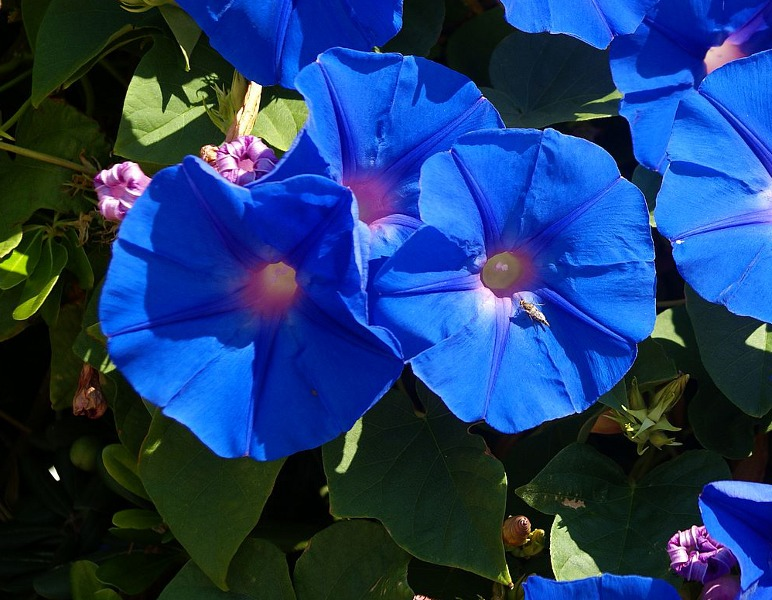
\includegraphics[width=2.5in]{images/segmentation/flowers.jpg}}
%   \end{minipage}% 
%   \begin{minipage}[t]{0.5\linewidth} 
%     \centering 
%     \subfloat[the ROI]{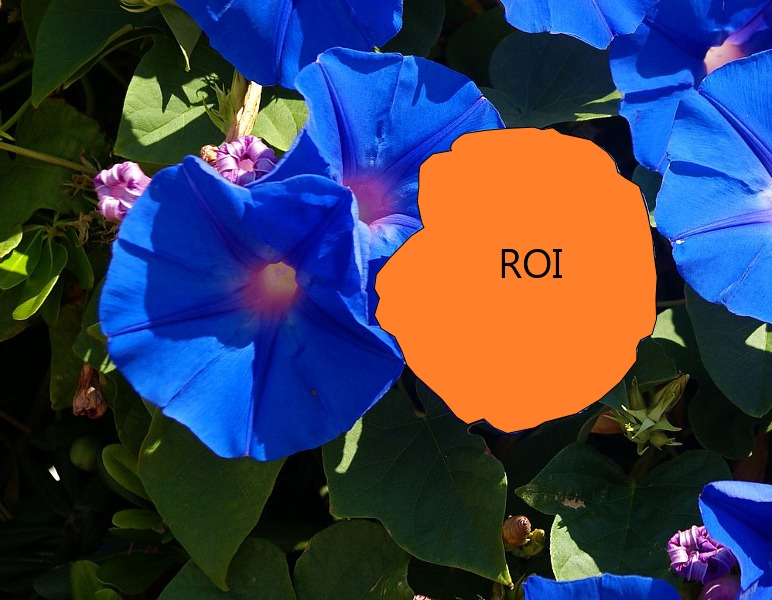
\includegraphics[width=2.5in]{images/segmentation/flowers_m.jpg}}
%   \end{minipage}
% \caption[Segmentation a flower petal from a cluster of flowers]{The
%   origin image is a little clutter, the border of the ROI in b) can
%   not be completely distinguished from the background due poor
%   contrast and shading.}
% \label{fig:flower_m}
% \end{figure}

There are many practical
applications of image segmentation, such as medical imaging, object
tracking, face recognition, fingerprint recognition, machine vision and
so on. In this thesis, we are concerned with object tracking mainly.
In many cases segmentation is the bottleneck when trying to track an
object. Many segmentation methods have been developed, however, there is not
general solution to the segmentation problem. In the real world,
segmentation problems will often require much domain knowledge before
a successful segmentation can be performed. The CCD algorithm is a
powerful method which is combined with the prior knowledge. By
converting a pure segmentation problem to a problem from pattern
recognition field, a large amount of techniques in the field of pattern
recognition are introduced to solve segmentation problems, which are
proved to be effective and helpful. In comparison with other segmentation
methods, such as
edge detection (Fig.~\ref{fig:seg_comparison}a), watershed
transformation methods (Fig.~\ref{fig:seg_comparison}b), graph
partitioning methods (Fig.~\ref{fig:seg_comparison}c)
and cluster methods (Fig.~\ref{fig:seg_comparison}d and Fig.~\ref{fig:seg_comparison}e),
, the CCD algorithm has following advantages:
\begin{figure}[htbp] 
  \begin{minipage}[t]{0.5\linewidth} 
    \centering 
    \subfloat[Sobel]{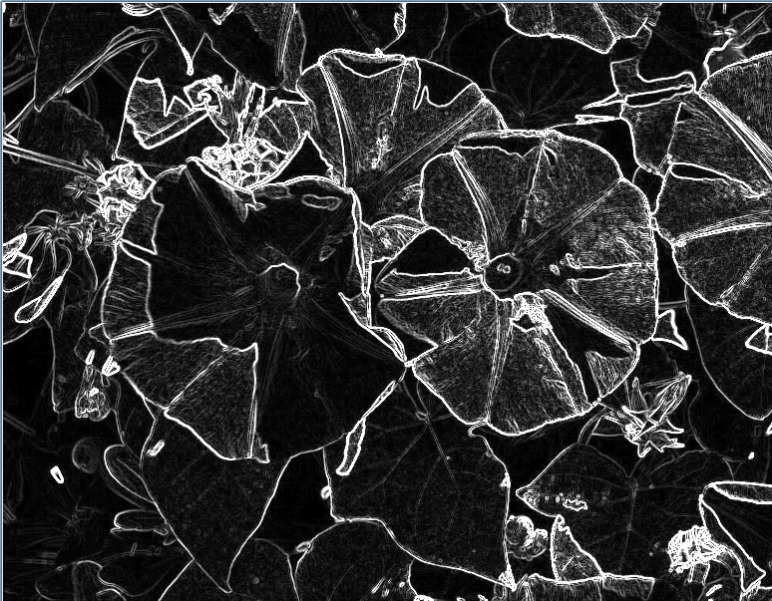
\includegraphics[width=2.5in]{images/flowers_sobel.jpg}}
  \end{minipage} 
  \begin{minipage}[t]{0.5\linewidth} 
    \centering 
    \subfloat[Watershed algorithm]{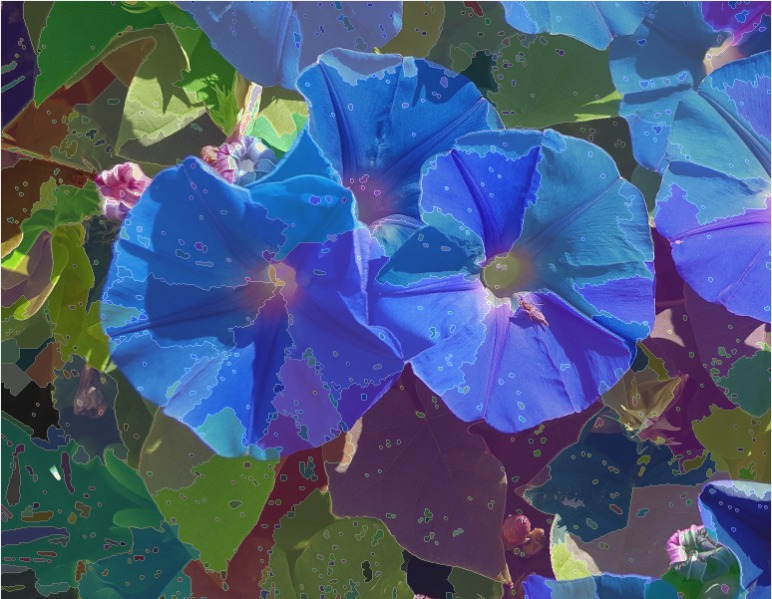
\includegraphics[width=2.5in]{images/flowers_watershed.jpg}}
  \end{minipage} 
  \begin{minipage}[t]{0.5\linewidth} 
    \centering 
    \subfloat[Graph cut]{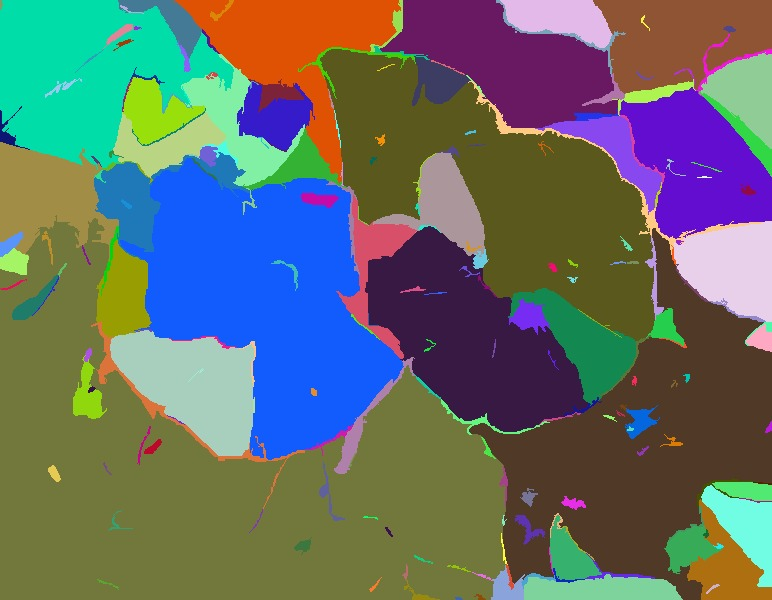
\includegraphics[width=2.5in]{images/flowers_graph.jpg}}
  \end{minipage} 
  \begin{minipage}[t]{0.5\linewidth} 
    \centering 
    \subfloat[Kmeans++]{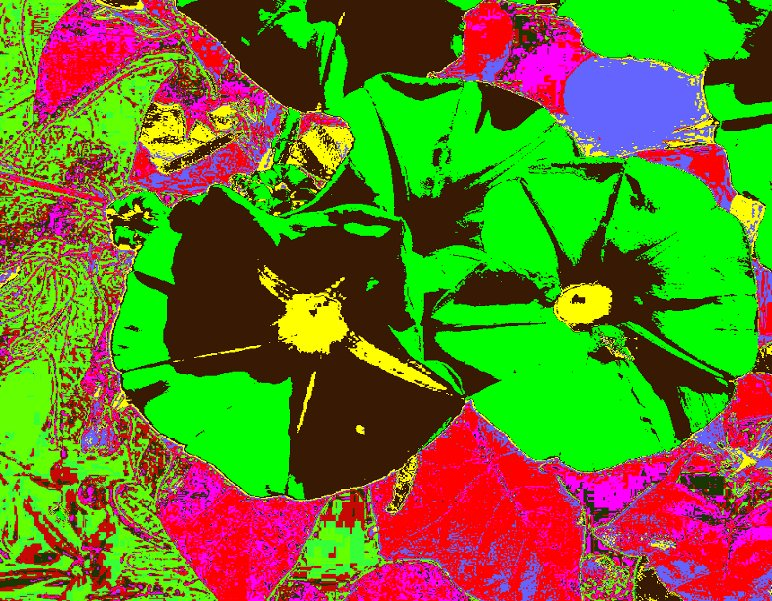
\includegraphics[width=2.5in]{images/flowers_kmeans.jpg}}
  \end{minipage} 
  \begin{minipage}[t]{0.5\linewidth} 
    \centering 
    \subfloat[Expectation and Maximization]{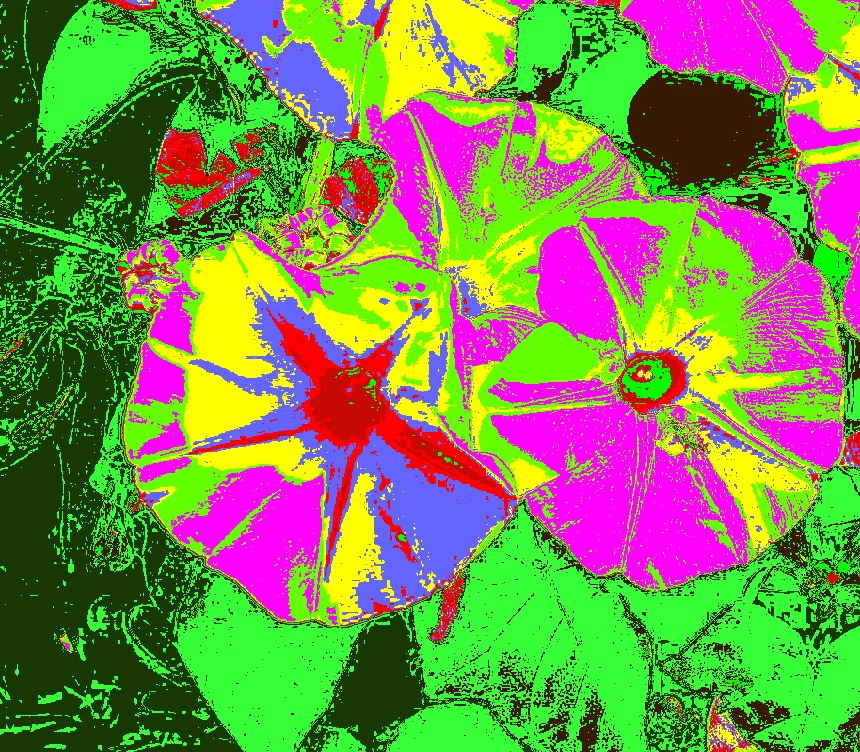
\includegraphics[width=2.5in]{images/flowers_em.jpg}}
  \end{minipage}
  \begin{minipage}[t]{0.5\linewidth} 
    \centering 
    \subfloat[CCD]{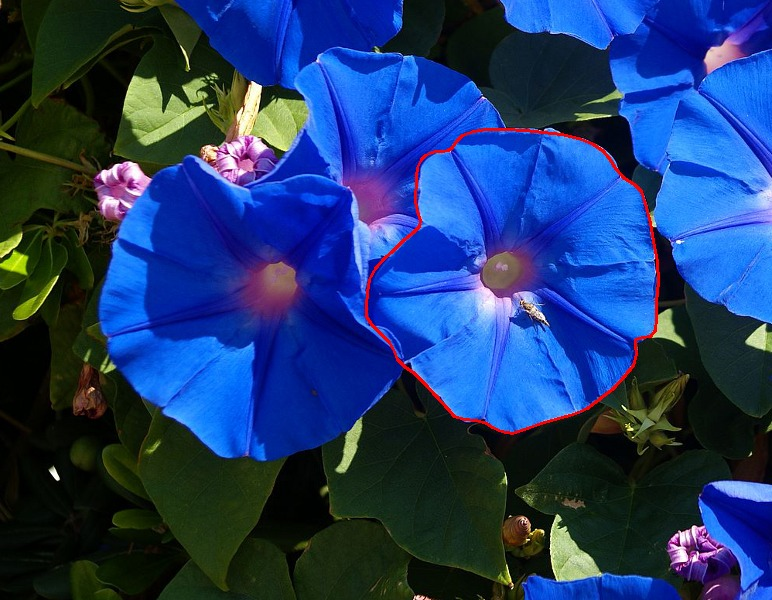
\includegraphics[width=2.5in]{images/flowers_ccd.jpg}}
  \end{minipage}% 
\caption[Resulting images after applying some segmentation methods]{a)
  Edges are detected by a gradient-based algorithm~\cite{scharr2000optimal}. b) Watershed algorithm takes an image as a
  topographic relief. c) Segmentation of an image by defining a predicate for
  measuring the evidence for a boundary between two regions using a
  graph-based representation of the
  image~\cite{felzenszwalb2004efficient}. d) K-means++ algorithm is a
  cluster-based segmentation algorithm~\cite{arthur2007k}. e)
  Segmentation result of Expectation-Maximization (EM) algorithm,
  usually it is initialized by K-means algorithm~\cite{bishop2006pattern}. f) the contour segmented by the CCD
  algorithm discussed in this thesis.}
\label{fig:seg_comparison}
\end{figure}

\begin{itemize}
\item restrict segmentation problem to a limited explicit region: it is helpful
  to decrease the computational cost;
\item probabilistic representation of the variation of the registered
  samples could be easily given, thus statistical inference between
  the model and the image will be applied. All these are helpful to
  improve the segmentation results;
\item the CCD algorithm achieves sub-pixel accuracy and high
  robustness because only a relatively small fraction of the pixels is
  taken into account in the end of iteration.
\end{itemize}

\begin{figure}[htbp] 
  \begin{minipage}[t]{0.5\linewidth} 
    \centering 
        \subfloat[iteration 1]{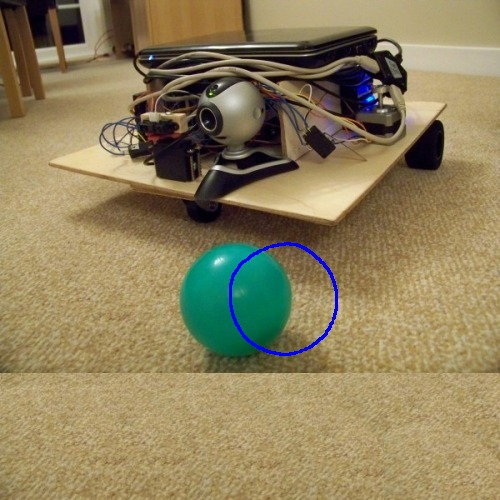
\includegraphics[width=2.5in]{images/ball/0.jpg}}
  \end{minipage}% 
  \begin{minipage}[t]{0.5\linewidth} 
    \centering 
    \subfloat[iteration 3]{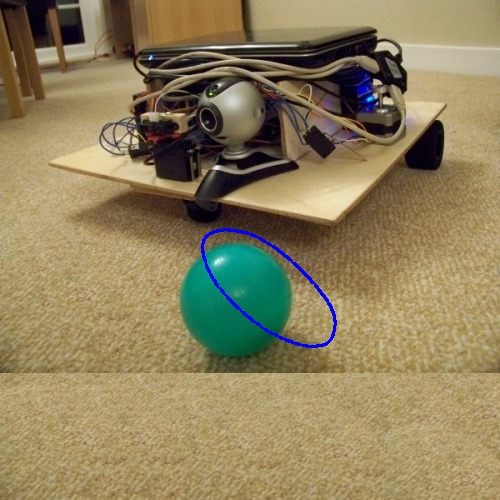
\includegraphics[width=2.5in]{images/ball/2.jpg}}
  \end{minipage} 
  \begin{minipage}[t]{0.5\linewidth} 
    \centering 
    \subfloat[iteration 7]{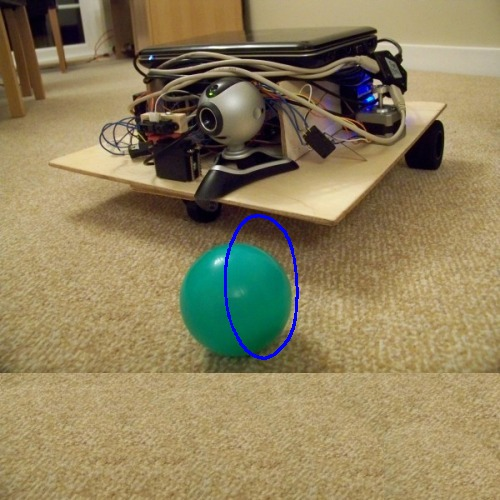
\includegraphics[width=2.5in]{images/ball/6.jpg}}
  \end{minipage} 
  \begin{minipage}[t]{0.5\linewidth} 
    \centering 
    \subfloat[iteration 16]{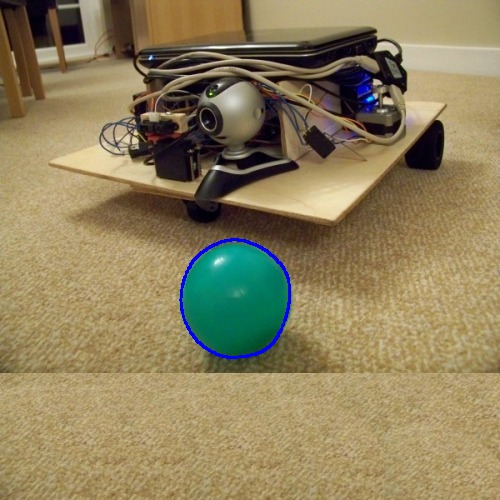
\includegraphics[width=2.5in]{images/ball/15.jpg}}
  \end{minipage} 
\caption[Segmentation of a ball] {a) Rough initialization with the
  mandatory condition that the curve encompasses at least the part of
  the object. b, c) In the beginning, the uncertainty of
  the contour is very large, so the contour is always changing in
  affine-space. After several iterations, it starts to converge and, 
  d) successfully snaps to the obejct.
\label{fig:sab}
}
\end{figure}

In the following, we apply the proposed CCD algorithm to 4 kind of
objects:
\begin{enumerate}
\item segmentation of a spherical object;
\item segmentation of a three-dimensional object;
\item segmentation of a half-transparent object;
\item fitting a rigid wire frame.
\end{enumerate}

\subsection{Segmentation of a Ball}
\label{sec:sb}
\begin{figure}[htbp] 
  \begin{minipage}[t]{0.5\linewidth} 
    \centering 
    \subfloat[iteration 1]{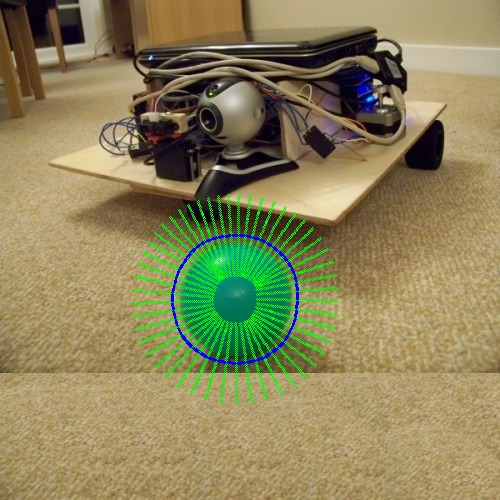
\includegraphics[width=2.5in]{images/ball_normal/0.jpg}}
  \end{minipage}% 
  \begin{minipage}[t]{0.5\linewidth} 
    \centering 
    \subfloat[iteration 3]{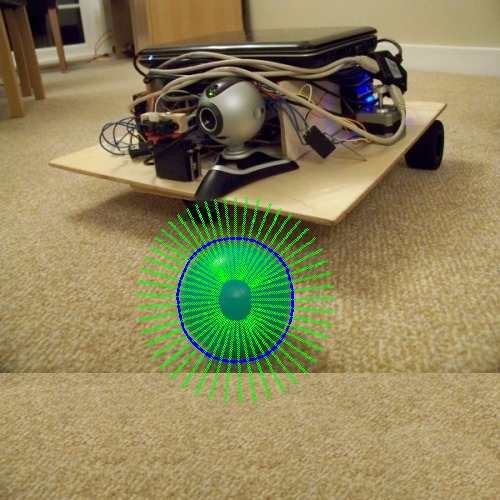
\includegraphics[width=2.5in]{images/ball_normal/1.jpg}}
  \end{minipage} 
  \begin{minipage}[t]{0.5\linewidth} 
    \centering 
    \subfloat[iteration 5]{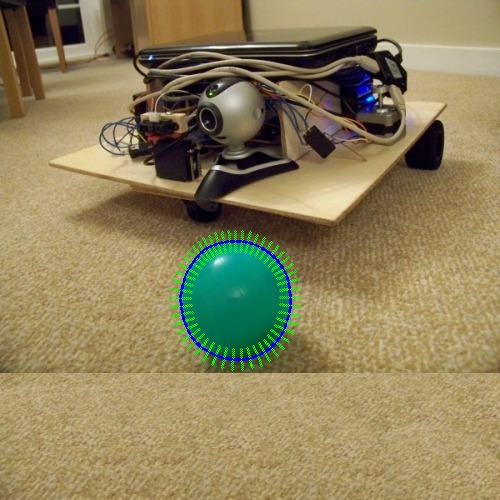
\includegraphics[width=2.5in]{images/ball_normal/3.jpg}}
  \end{minipage} 
  \begin{minipage}[t]{0.5\linewidth} 
    \centering 
    \subfloat[iteration 6]{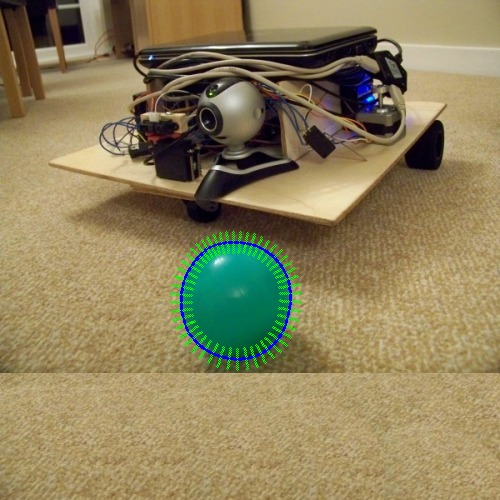
\includegraphics[width=2.5in]{images/ball_normal/4.jpg}}
  \end{minipage} 
\caption[Pixels used in each iteration]{Only a small number of pixels are taken into account after the
contour starts to converge but these pixels contain all the
necessary information for refinement of the fitting. Because the
number of sample points used to compute local statistics 
becomes less and less, only a small number of pixels near the boundary
are considered. This makes the CCD algorithm achieve high
sub-pixel accuracy.}
\label{fig:pon}
\end{figure}
Like other contour-based methods, we model a contour of the ball as the
prior knowledge. Because the contour for a rigid spherical object is a
circle, besides manually initialization, we can use built-in function in
OpenCV library to generate the contour with given center and
radius. According to the definition of prior distribution, it is required
that the hypothesis is in the range of the variation of
registered samples, namely, the initial contour can not be too far away
from the observed object.

In Fig.~\ref{fig:sab}, we intentionally set a hypothesis which is far away
from the ball, but after about 15 iterations, we successfully fit the
contour of the ball. % For the sake of a ground truth we need
% to investigate the pixels used in the iterations. 
Fig.~\ref{fig:pon} shows
that only a small number of pixels are taken into account after the
contour starts to converge but these pixels contain all the
necessary information for refinement of the fitting. Because the
number of sample points used to compute local statistics 
becomes less and less, only a small number of pixels near the boundary
are considered. This makes the CCD algorithm achieve high
sub-pixel accuracy.

\subsection{Segmentation of a Cuboid-shaped Object}
\label{sec:s3o}
In the experiments of segmenting a spherical object, a planar
affine space of contour is generated. It works very well because the
contour of the ball is always a circle, there is no parallax effect
for such objects. In this case, a six-dimensional model parameter vector
can cope with basic geometrical transformation of an object. However,
clearly a six-dimensional model parameter vector can not
suffice for non-planar surfaces. Imagine a scenario where we generate the  planar affine
space contour of a three-dimensional cube in the first view (Fig.~\ref{fig:box_mismatch}a). In the
subsequent view the cube does not lie in the old
space. Due to the parallax effect the mismatch in the fitted contour
will be detected. This is demonstrated in the fitting experiment (Fig.~\ref{fig:box_mismatch}).
\begin{figure}[htbp]
  \begin{minipage}[t]{0.5\linewidth} 
    \centering 
    \subfloat[]{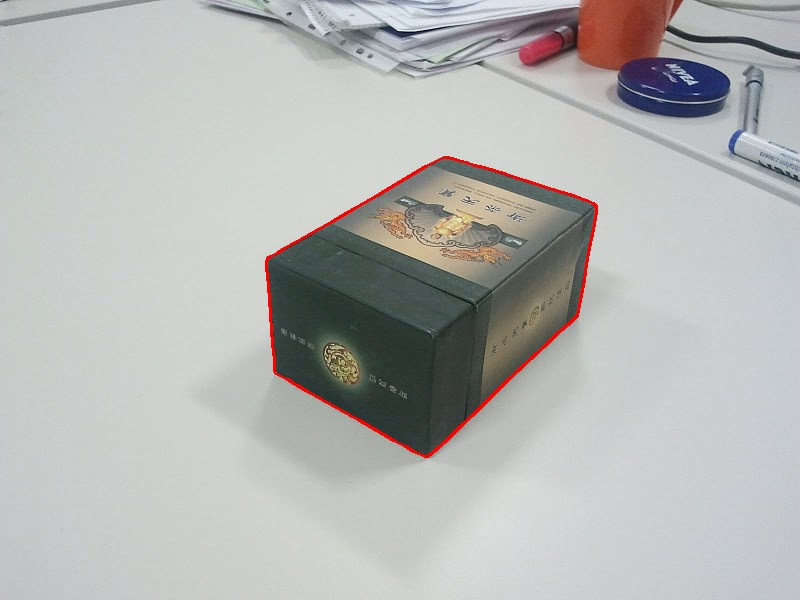
\includegraphics[width=2.5in]{images/box1.jpg}}
  \end{minipage}% 
  \begin{minipage}[t]{0.5\linewidth} 
    \centering 
    \subfloat[]{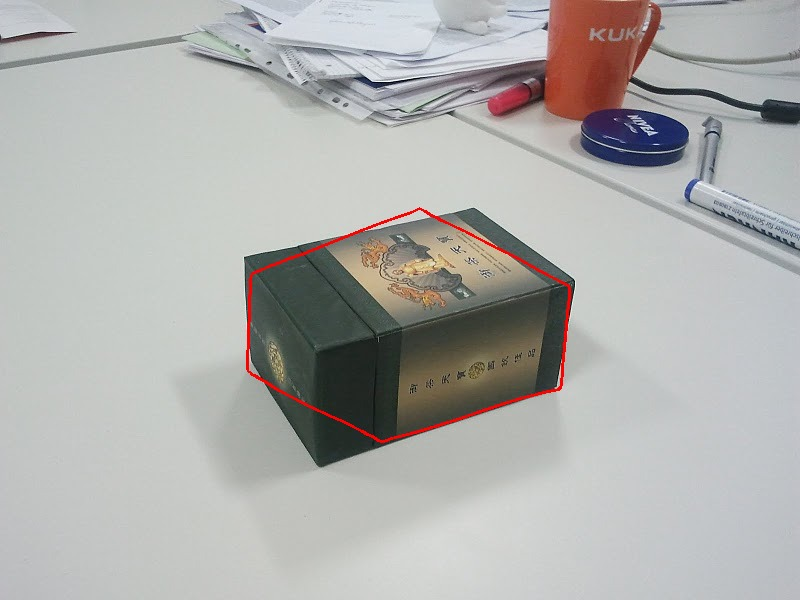
\includegraphics[width=2.5in]{images/box2_mismatch.jpg}}
  \end{minipage} 
  \caption[Planar space can not encompass a general three-dimensional
  contour]{a) A planar affine space of contours has been fitted from
    the outline of the first view of the cuboid. b) As the viewpoint
    is changed, the outline of the cuboid in the subsequent view does
    not lie in the affine space, which causes visible mismatch in the
    fitted contours.}
\label{fig:box_mismatch}
\end{figure}


% The new three-dimensional affine shape-space with 8 degree of freedom,
% made up of the 6-parameter planar affine space and a two-parameter
% extension, is designed to cope with such problem. 
In order to account for this issue we introduced the three-dimensional affine
shape-space with 8 DOFs.
Two added components
account for the depth variation that is not visible in the template
view. After adding the two new parameters to the shape matrix, the form
of shape matrix for three-dimensional case can be given as follows:
\begin{equation}
  \label{eq:4.18}
  A =
  \begin{bmatrix}
    1 & 0 & P_0^x & 0 & 0 & P_0^y & P_0^z & 0\\
    0 & 1 & 0 & P_0^y & P_0^x & 0 & 0  & P_0^z
  \end{bmatrix}\qquad.
\end{equation}

\begin{figure}[htbp]
  \begin{minipage}[t]{0.5\linewidth} 
    \centering 
    \subfloat[]{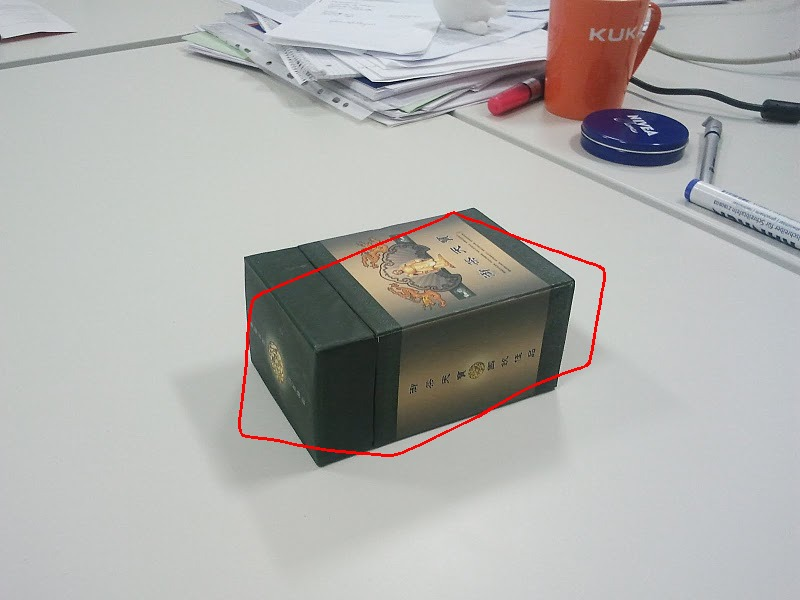
\includegraphics[width=2.5in]{images/box2_3d.jpg}}
  \end{minipage}% 
  \begin{minipage}[t]{0.5\linewidth} 
    \centering 
    \subfloat[]{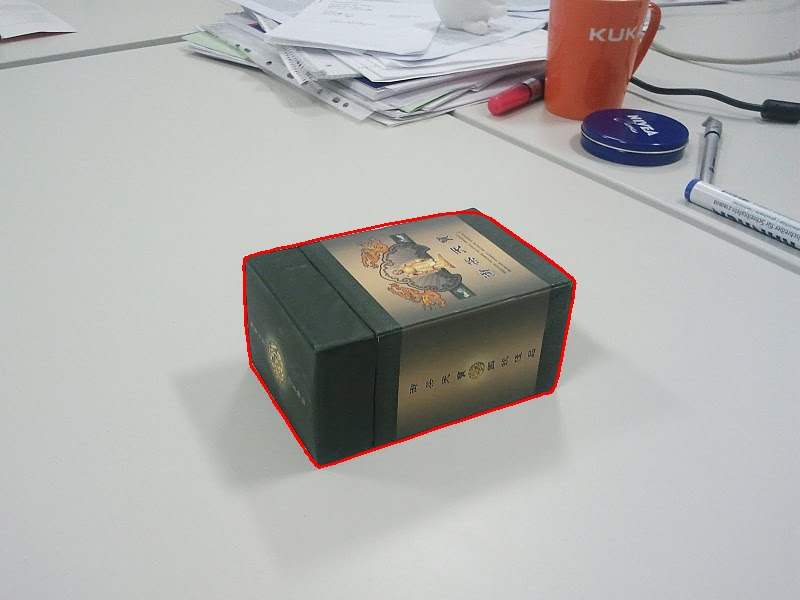
\includegraphics[width=2.5in]{images/box2_ok.jpg}}
  \end{minipage} 
  \caption[Fitting the contour of three-dimensional object]{Using three-dimensional
    affine shape-space fitting of a contour to the observed object
    becomes possible.}
\label{fig:box_match}
\end{figure}

The three-dimensional affine shape-space model parameters have
the following interpretation

\begin{equation}
  \label{eq:4.19}
  \mathbf{\Phi} =  (T_1, T_2, M_{11} - 1, M_{22} - 1, M_{21}, M_{12}, \nu_1, \nu_2)
\end{equation}

\begin{figure}[htbp] 
  \begin{minipage}[t]{0.5\linewidth} 
    \centering 
    \subfloat[iteration 1]{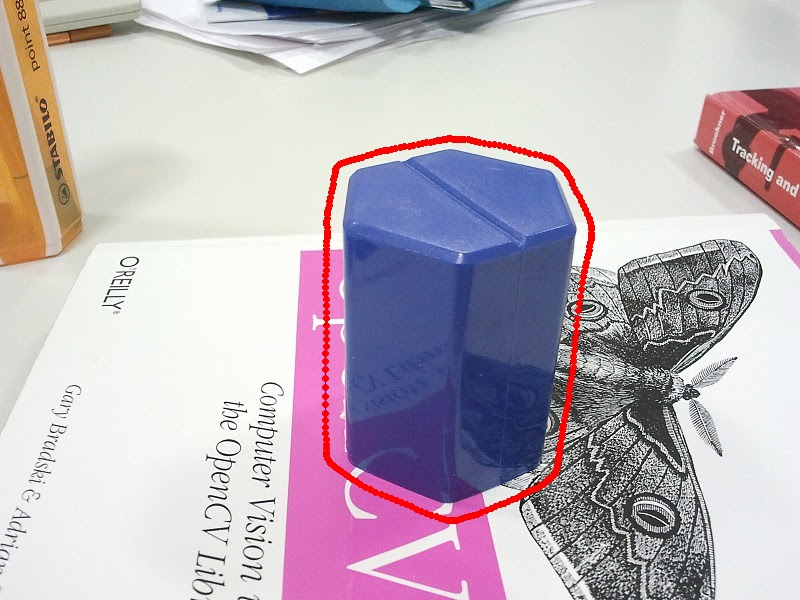
\includegraphics[width=2.5in]{images/container/0.jpg}}
  \end{minipage}% 
  \begin{minipage}[t]{0.5\linewidth} 
    \centering 
    \subfloat[iteration 2]{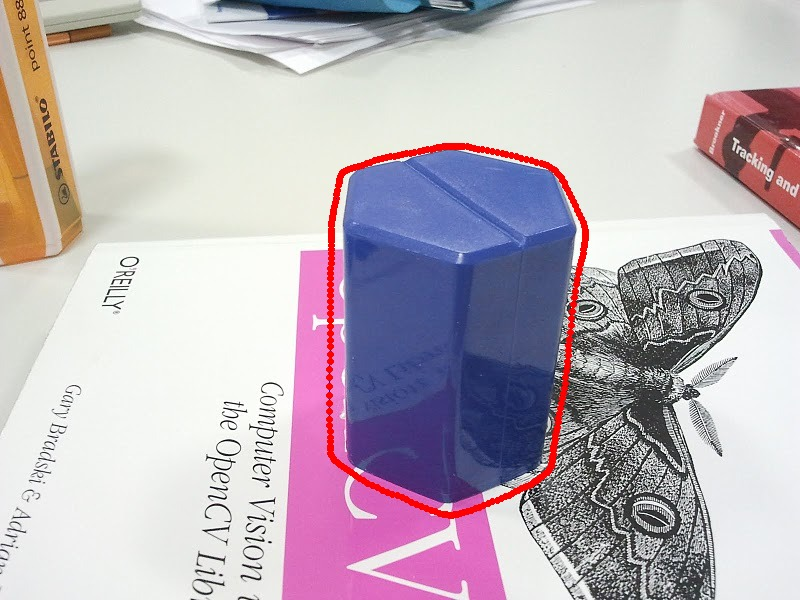
\includegraphics[width=2.5in]{images/container/1.jpg}}
  \end{minipage} 
  \begin{minipage}[t]{0.5\linewidth} 
    \centering 
    \subfloat[iteration 4]{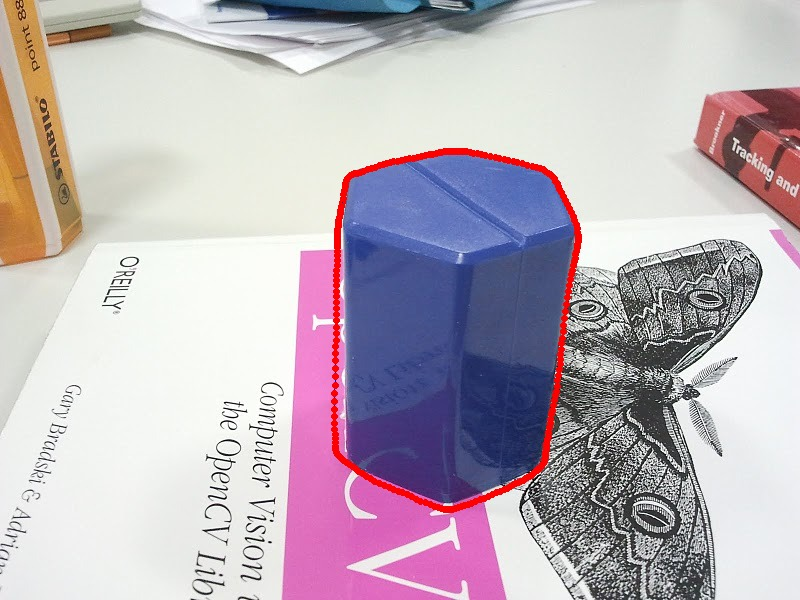
\includegraphics[width=2.5in]{images/container/2.jpg}}
  \end{minipage} 
  \begin{minipage}[t]{0.5\linewidth} 
    \centering 
    \subfloat[iteration 7]{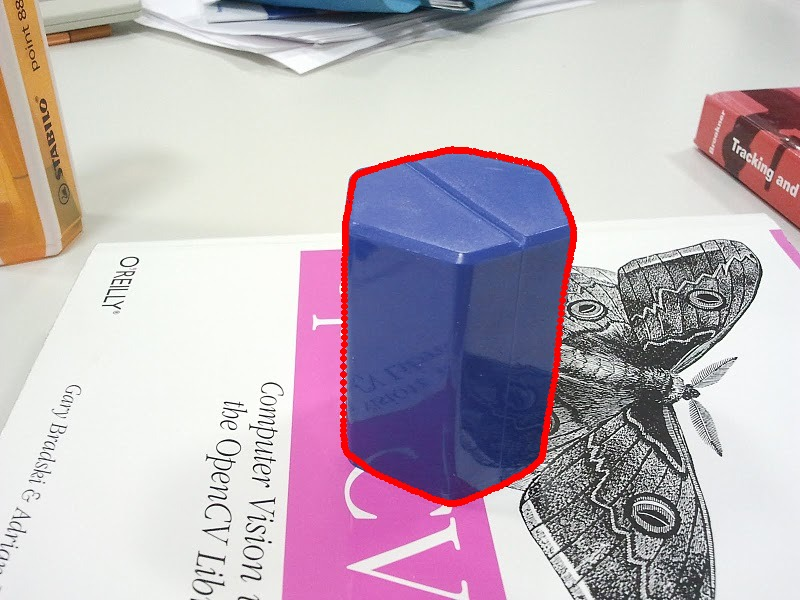
\includegraphics[width=2.5in]{images/container/5.jpg}}
  \end{minipage} 
\caption[three-dimensional affine shape-space for rigid object]{The
  non-planar polyhedron is encompassed by a three-dimensional affine space.}
\label{fig:container}
\end{figure}

The expanded space now encompasses the object in all views as depicted
in Fig.~\ref{fig:box_match}. At last, we do
another experiment for an object with an irregular shape (Fig.~\ref{fig:container}). This
demonstrates that the CCD works well for three-dimensional object,
too.
\subsection{Segmentation of a Transparent Object}
\label{sec:sto}
In this thesis, local statistical information is collected in terms of
pixel intensity in the vicinity of a contour, which leads to a poor
result for transparent objects. In this experiment, the
target is a Cocacola bottle whose upper part is nearly transparent and the
lower part is opaque. The result in Fig.~\ref{fig:cola} shows that the CCD algorithm
segments the lower part but fails to completely encompass the contour in the
upper part. However, because the model only has 6 (or 8
for three-dimensional object) DOFs, the convergence of the lower part will aid the convergence for the whole object.
\begin{figure}[htbp] 
  \begin{minipage}[t]{0.5\linewidth} 
    \centering 
    \subfloat[iteration 1]{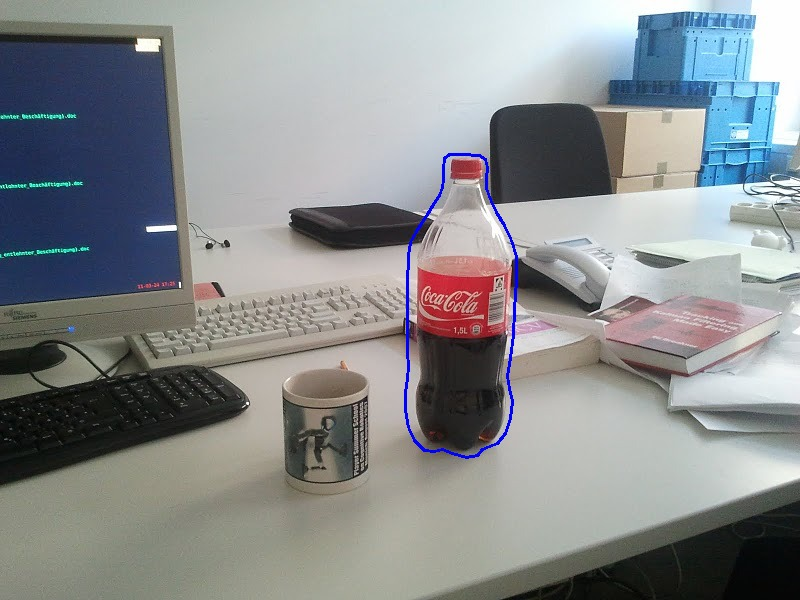
\includegraphics[width=2.5in]{images/bottle/0.jpg}}
  \end{minipage}% 
  \begin{minipage}[t]{0.5\linewidth} 
    \centering 
    \subfloat[iteration 2]{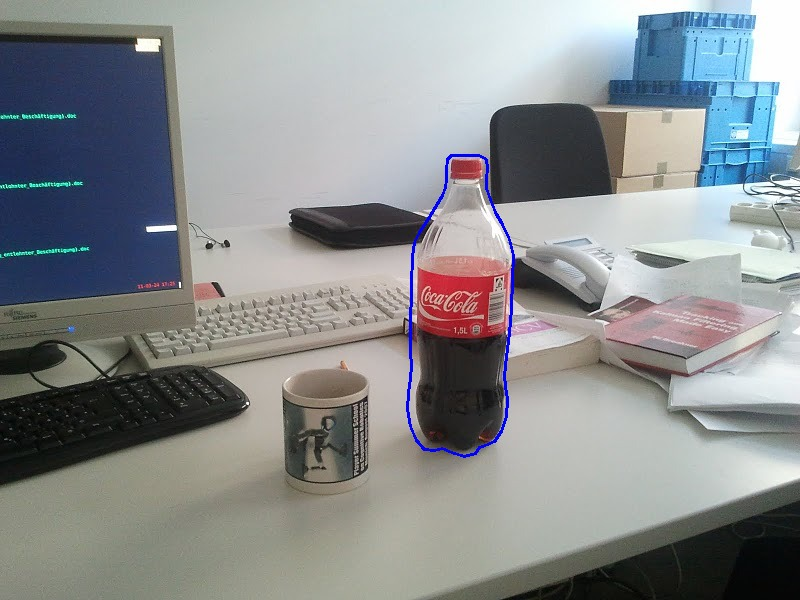
\includegraphics[width=2.5in]{images/bottle/1.jpg}}
  \end{minipage} 
  \begin{minipage}[t]{0.5\linewidth} 
    \centering 
    \subfloat[iteration 3]{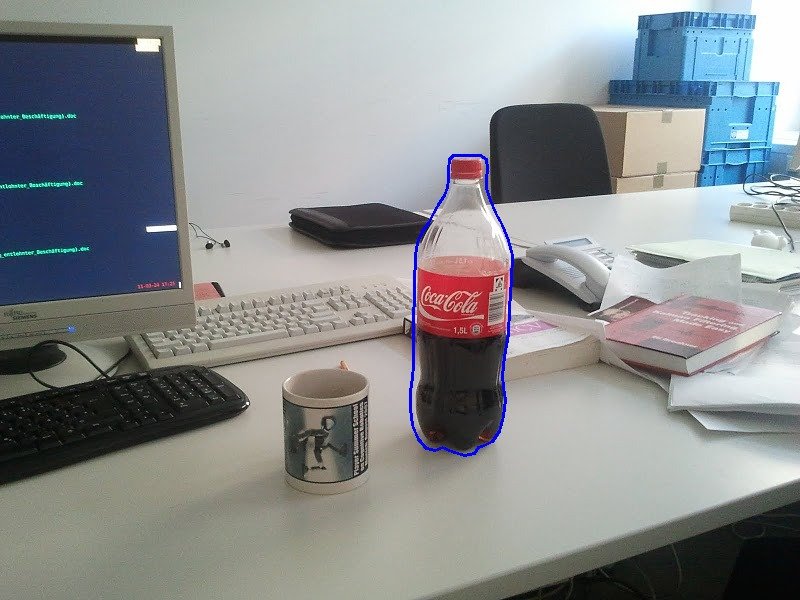
\includegraphics[width=2.5in]{images/bottle/2.jpg}}
  \end{minipage} 
  \begin{minipage}[t]{0.5\linewidth} 
    \centering 
    \subfloat[iteration 21]{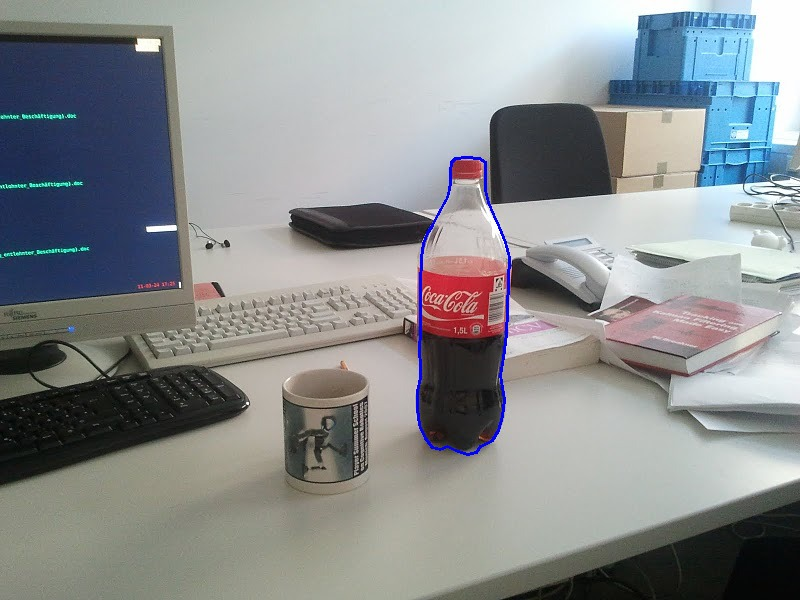
\includegraphics[width=2.5in]{images/bottle/20.jpg}}
  \end{minipage} 
\caption[An example of a successful convergence for the half-transparent object]{An example of a
  successful convergence for the half-transparent object. In image (d), due to the shadow and poor
contrast, the contour does not completely attach to the edge of the
bottom. Moreover, in the transparent part of the bottle, the outline
closely attaches to the edge in the left but stays away from the edge
in the right. The transparency leads to the difficulties. }
\label{fig:cola}
\end{figure}
% \subsection{Fitting a Rigid Wire Frame}
% \label{sec:fdo}
% In the following, we fit a rigid wire frame model to the image
% depicted in Fig.~\ref{fig:wireframe}.  The DOFs
% are the 8 pose parameters. This experiment demonstrates that the CCD
% algorithm is not only able to exploit object contours, but it can also
% use internal model edges separating multiple, possibly dependent,
% image regions.  The CCD algorithm reliably estimates the pose of the box despite
% the partial occlusion.

% \begin{figure}[htbp] 
%   \begin{minipage}[t]{0.5\linewidth} 
%     \centering  
%     \subfloat[iteration 1]{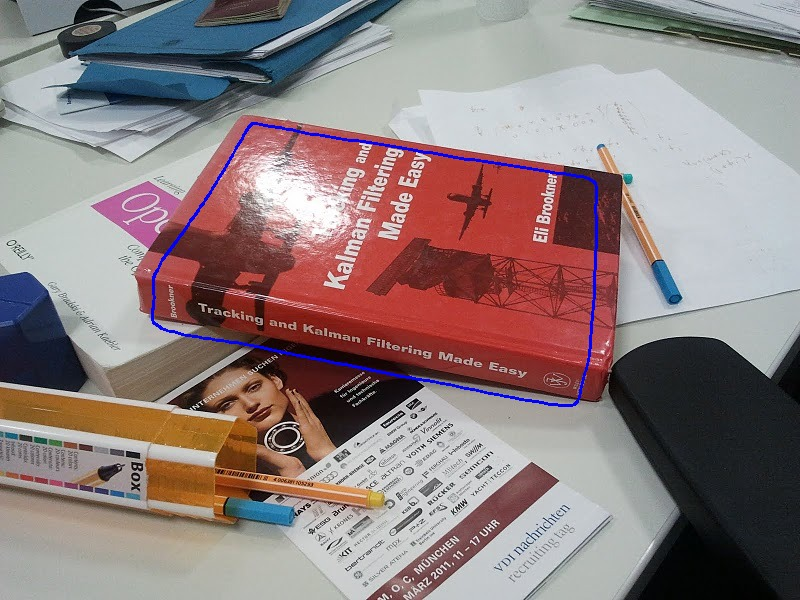
\includegraphics[width=2.5in]{images/book/0.jpg}}    
%   \end{minipage}% 
%   \begin{minipage}[t]{0.5\linewidth} 
%     \centering 
%     \subfloat[iteration 2]{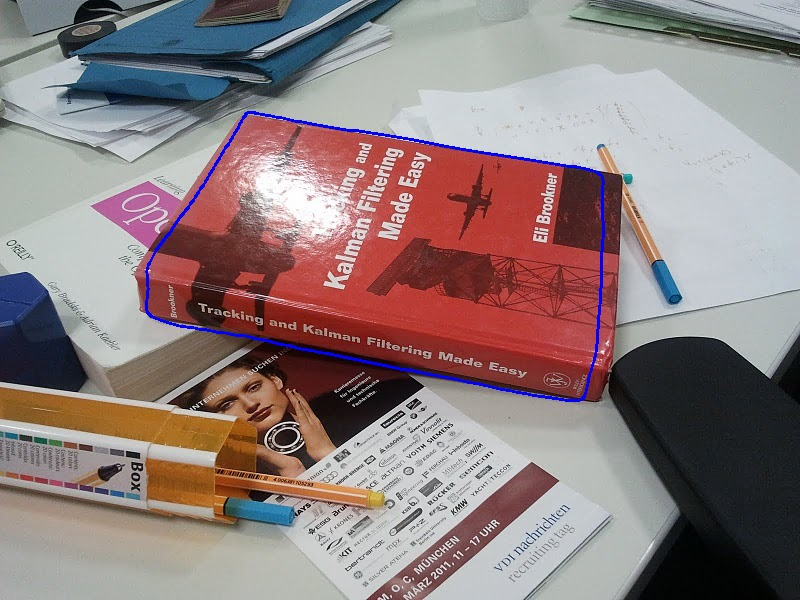
\includegraphics[width=2.5in]{images/book/1.jpg}}
%   \end{minipage} 
%   \begin{minipage}[t]{0.5\linewidth} 
%     \centering 
%     \subfloat[iteration 3]{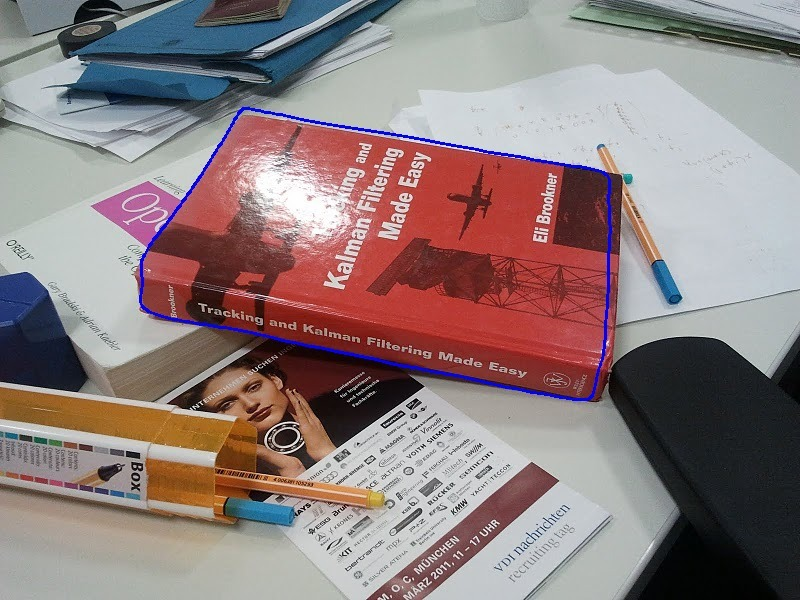
\includegraphics[width=2.5in]{images/book/2.jpg}}
%     \label{subfig:iteration 3}
%   \end{minipage} 
%   \begin{minipage}[t]{0.5\linewidth} 
%     \centering 
%     \subfloat[iteration 14]{\includegraphics[width=2.5in]{images/book/13.jpg}}
%   \end{minipage}
%   \begin{minipage}[t]{\linewidth} 
%     \centering 
%     \subfloat[segmentation of edge-based algorithm]{\includegraphics[width=0.8\linewidth]{images/book/book_sobel.jpg}}
%   \end{minipage} 
% \caption[Fitting a rigid wire frame in a inhomogeneous background]{The book
%   is located in a partially occluded background. From (a)-(d), despite
% the variation of the illumination and contrast, the CCD algorithm
% accurately fits a wire frame model to the image data. In (e), here the
% edge-based algorithm yields some errors.}
% \label{fig:wireframe}
% \end{figure}

\section{Tracking Initialized Manually}
\begin{figure}[htbp]
  \begin{minipage}[t]{0.5\linewidth} 
    \centering  
    \subfloat[Control points initialized manually]{\includegraphics[width=2.5in]{images/plate/1.jpg}}    
  \end{minipage}% 
  \begin{minipage}[t]{0.5\linewidth} 
    \centering 
    \subfloat[Initial B-spline contour]{\includegraphics[width=2.5in]{images/plate/2.jpg}}
  \end{minipage} 
  \begin{minipage}[t]{0.5\linewidth} 
    \centering 
    \subfloat[Frame 1]{\includegraphics[width=2.5in]{images/plate/3.jpg}}
  \end{minipage} 
  \begin{minipage}[t]{0.5\linewidth} 
    \centering 
    \subfloat[Frame 50]{\includegraphics[width=2.5in]{images/plate/4.jpg}}
  \end{minipage} 
  \begin{minipage}[t]{0.5\linewidth} 
    \centering 
    \subfloat[Frame 100]{\includegraphics[width=2.5in]{images/plate/5.jpg}}
  \end{minipage} 
  \begin{minipage}[t]{0.5\linewidth} 
    \centering 
    \subfloat[Frame 144]{\includegraphics[width=2.5in]{images/plate/6.jpg}}
  \end{minipage} 
  \caption[Tracking initialized manually]{Tracking initialized
    manually: a) Manually draw some control points, the contour is not
    required to  be closed the edge of the object. Now approximately
    it is a ellipse. b) The B-spline
    curve generated from the interpolation of the control points. c) -
    f) The results of frame 1, 50, 100, 144.
  }
  \label{fig:plate}
\end{figure}
In this experiment, we use the CCD approach to track a plate on a
table and analyze the experimental results. 
In Fig.~\ref{fig:plate}, apparently, the tracker has successfully
captured the contour of the observed plate. However, we find that the
contour does not completely encompass the edge of the object in the
beginning of the motion. The edge of the plate is analyzed by the
Sobel operator, it is shown that the edge in that region is not
sharp. Moreover, the pixels values of the shadow is
close to and the ones of the edge of the plate (Fig. ~\ref{fig:rgb}). Hence,
the contour can not snap to the edge. But the changes of the control
points in this region have not changed the shape of the whole
contour, because the contour has limited DOFs. There are two solution
for this problem:
\begin{itemize}
\item Using other local statistics based on other features to replace
  the RGB statistics.
\item Sharpen the edge of the observed object.
\end{itemize}

\begin{figure}[htbp]
  \centering
  \includegraphics[width=12cm]{images/edge.jpg}
  \caption[Shadow effects]{The contour does not completely encompass
    the edge because of shadow effects.}
  \label{fig:rgb}
\end{figure}

\section{Track Initialization from SIFT Features}
\label{sec:sift_init}
\begin{figure}[htbp]
  \centering
\includegraphics[width=12cm]{images/sift_result.jpg}
\caption[The contour obtained using the CCD algorithm converges to the
edge of the book]{After 8 iterations, the contour obtained in Fig.~\ref{fig:sift} converges to the edge of the book.}
\label{fig:sift_result}
\end{figure}
Scale-invariant feature transform (or SIFT) is an algorithm to detect
and describe local features in images.  It is widely used to solve
many problems in the field of Computer Vision, such as object
recognition, robotic mapping and navigation, and video tracking. There are four key stages in the sift algorithm~\cite{lowe2004distinctive}:
\begin{enumerate}
\item \textbf{Scale-invariant feature detection}: an image is transformed into
  a collection of vectors which are scale-invariant. By applying a Difference-of-Gaussian
function to a series of smoothed and resampled images, potential
interest points are identified.
\item \textbf{Keypoint localization and indexing}: keypoints are selected at given
  candidate location, and then stored as SIFT keys.
\item \textbf{Orientation assignment}:  one or more orientations are assigned to each keypoint lo-
cation based on local image gradient directions. All future operations are performed
on image data that has been transformed relative to the assigned orientation, scale, and
location for each feature, thereby providing invariance to these transformations.
\item \textbf{Keypoint descriptor}: the local image gradients are measured at the selected scale
in the region around each keypoint. These are transformed into a representation that
allows for significant levels of local shape distortion and change in illumination.
\end{enumerate}


The SIFT keypoints and features are local and based on the appearance
of the object at particular interest points. The SIFT algorithm has following
features and advantages:
\begin{itemize}
\item Invariant to image scale and rotation, robust to changes in
  illumination and minor changes in viewpoint.
\item Highly distinctive, easy to extract, allow for correct object
  identification and easy to match against a database of local
  features. 
\item Need few features (as few as 3) from an object to compute its location
  and pose. Computational cost is moderate on modern computer hardware.
\end{itemize}

% Based on these features, SIFT is usable for object recognition, the
% steps are given below.
% \begin{itemize}
% \item Extract SIFT features from a series of input template image,
%   then store these features into a database.
% \item Given a new input image, after training, the features in
%   the image are matched to the SIFT feature database obtained from the
%   training images.
% \end{itemize}

\begin{figure}[htbp]
  \centering
\includegraphics[width=12cm]{images/sift.jpg}
\caption[Contour initialization using the SIFT algorithm]{The image in
  the upper-left corner is a template. It is projected into the bottom
  image. The green points in the template image encompass the
  contour of the observed object. The red lines are used to connect the matching feature
  points. Obviously, the outliers are excluded using the RANSAC
  algorithm. The homography is then estimated from these matching
  feature points.  After finding a perspective
  transformation from the matching features, the source contour is
  projected onto the image in the bottom, and used as initial contour
  for the CCD algorithm.}
\label{fig:sift}
\end{figure}

In this thesis, we use the SIFT algorithm to initialize the
contour of an object. Assume we have marked the boundary points in the
training images. In order to project these boundary points to the test
image, it is essential to estimate the homography between the
images. However, SIFT matching
might lead to lots of "false" matches. % In order
% to evaluate the homography, firstly we have to exclude the
% mismatches. 
For filtering out false positives, we use \acronym{RANSAC}{RANdom SAmple Consensus}, which is an
iterative process that randomly selects enough matches to fit the
homography. It contains the following steps~\cite{fischler1981random}.

\begin{figure}[htbp]
  \begin{minipage}[t]{0.5\linewidth} 
    \centering  
    \subfloat[Sampled frame 1]{\includegraphics[width=2.5in]{images/sift/1.jpg}}    
  \end{minipage}% 
  \begin{minipage}[t]{0.5\linewidth} 
    \centering 
    \subfloat[Sampled frame 2]{\includegraphics[width=2.5in]{images/sift/10.jpg}}
  \end{minipage} 
  \begin{minipage}[t]{0.5\linewidth} 
    \centering 
    \subfloat[Sampled frame 3]{\includegraphics[width=2.5in]{images/sift/30.jpg}}
    \label{subfig:iteration 3}
  \end{minipage} 
  \begin{minipage}[t]{0.5\linewidth} 
    \centering 
    \subfloat[Sampled frame 4]{\includegraphics[width=2.5in]{images/sift/45.jpg}}
  \end{minipage} 
  \begin{minipage}[t]{0.5\linewidth} 
    \centering 
    \subfloat[Sampled frame 5]{\includegraphics[width=2.5in]{images/sift/63.jpg}}
  \end{minipage} 
  \begin{minipage}[t]{0.5\linewidth} 
    \centering 
    \subfloat[Sampled frame 6]{\includegraphics[width=2.5in]{images/sift/80.jpg}}
  \end{minipage} 
  \caption[The tracking result based on SIFT contour initialization]{The
    CCD tracker successfully tracks the motion of a book.
  }
  \label{fig:sifttracker}
\end{figure}

\begin{itemize}
\item  Randomly select a sample of matched points and instantiate the
  model from this subset.
\item Determine the set of data points that are within a distance
  threshold of the homography. The set is the consensus set of the sample
  and defines the inliers.
\item If the size of the set (e.g. the number of inliers) is greater
  than some threshold, re-estimate the homography using all the matched
  points and terminate. Otherwise, select a new subset and repeat the
  above.
\item After some trials the largest consensus set is selected, and the
  homography is re-estimated using all the points in the subset.
\end{itemize}
Fast way to compute the homography in a least squares sense is to use the Normalized
Direct Linear Transform (normalized
\acronym{DLT}{Direct Linear Transform})~\cite{hartley2003multiple}. The Normalized DLT algorithm computes
a homography for a projective transformation by using at least 4 point
correspondences and then minimizing corresponding norm.

After obtaining the homography between the template image and the
test image, the contour of object can be easily projected
into the test image to obtain the estimate of the contour
position. This is illustrated in Fig.~\ref{fig:sift} and
Fig.~\ref{fig:sift_result}. Note that because SIFT is only invariant
to minor changes in view points, the method does not always work for
three-dimensional objects which have substantially different view points.

% The model hypothesis is obtained by applying the CCD algorithm to a
% frame of a video sequence. In the following experiments, we can test
% our naive CCD tracker on PR2, the result is demonstrated in Fig.~\ref{fig:sifttracker} 


\begin{figure}[htb]
  \centering
  \includegraphics[width=12cm]{images/pr2b.jpg}
  \caption[Kinect camera of the PR2 Robot and object candidate
  segmented in three-dimensional point cloud.]{Kinect camera of
    the PR2 Robot and object candidate segmented in three-dimensional point
    cloud. Encompassing a contour of the back-projected points onto
    the image is used as an initial contour for the CCD algorithm.}
  \label{fig:pointcloud}
\end{figure}
\section{Track Initialization from Three-dimensional Point Cloud}
\label{sec:tifpc}

% A point cloud is a set of vertices created by three-dimensional
% scanners. The scanners measure points on the surface of an object,
% therefore, a point cloud represents the set of points measured by the
% device. Point clouds cloud are widely used to  create three-dimensional CAD models
% for manufactured parts, a multitude of visualization, animation and
% rendering.
% Point clouds can be rendered and inspected in software like MeshLab
% and rviz (Fig.~\ref{fig:pointcloud}). In addition, they are usually converted to polygon or
% triangle mesh models, NURBS surface models, or CAD models through a
% process commonly referred to as surface reconstruction.

In this section, we describe an initialization method which utilizes three-dimensional
point cloud for finding contours.

As depicted in Fig.~\ref{fig:pointcloud}, the PR2 robot simultaneously takes a three-dimensional scan and captures
an image of the scene in front of it. The robot generates
object hypotheses by detecting candidate point clusters in
the three-dimensional point cloud acquired by the depth sensor. % These
% object hypotheses are then back-projected into the captured
% image as regions of interest and searched for detecting and
% recognizing objects.
The identified point clusters in the
point cloud are then back-projected into the captured image
to form the region of interest that corresponds to the object
candidate. An accurate back-projection is possible thanks to
the accurate robot calibration. The sensors are calibrated using a non-linear bundle-
adjustment-like optimization to estimate various parameters
of the PR2 Robot. However,
the resulting polygons of the observed object are not smoothed,
usually it can not completely encompass the whole object.
By applying the CCD algorithm, we can accurately obtain the contour of
a observed object. The result of the experiment is similar to the one
obtained from the SIFT features.
%  In
% comparison with the initialization from SIFT features, because the
% outlines created from point cloud is three-dimensional, it is more
% suitable for non-planar objects.

                %%% Local Variables: 
%%% mode: latex
%%% TeX-master: "../main"
%%% End: 

\chapter{Conclusion and  Future Work}
\label{chapter:conclusion}

\section{Conclusion}
\label{sec:con}

In this work, we have investigated the Contracting Curve Density (CCD)
algorithm and its application on personal robotics. Starting from
parametric model curve, we have analyzed the core of the algorithm and
proposed some improvements and optimizations on it. Then we applied the
algorithm on some challenging computer vision problems, such as curve
fitting, object segmentation and tracking, 3-D pose estimation. We
delivered some experiments on the PR2 robot which are showing satisfactory results. 

The CCD algorithm is an iterative procedure to refine an
a prior distribution of the model parameters to a Gaussian
approximation of the posterior distribution. It aims to extract the
contour of an object based a prior model. A MAP estimate need to be
evaluated by applying an effective local optimization method in order to get
the mean of model parameters and covariance matrices which govern the
posterior distribution and determine the shape of model. Likelihood is 
obtained from local statistics of the vicinity of the expected
curve. The local statistics provides locally adapted criteria for
adjacent image regions seperated by a contour. This criteria is stable
and effective than those relying on homogeneous image regions or
specific edge properties. The local statistics are very
important for the CCD algorithm, in this thesis we design a new weight
function as criteria for separating adjacent image regions. 
 In order to improve the performance and
reduce computing cost, a blurred curve model~\cite{hanek2004contracting} is applied as an efficient means for
iteratively optimization. In the iteration process, after the
algorithm starts to converge, the area of
convergence becomes smaller and smaller. This has two great
advantages, one is that the pixels used to learn the local statistic
are scaled, thus computing cost is decreased. Another one is that it
leads a high level sub-pixel accuracy. The decreasing rate of the
convergence area is significant, if too fast, the algorithm will stop
converging, on the other hand, if too slow, it is difficult to achieve
notably performance improvement. In this thesis we have investigated the relation between
the rate and the convergence speed.
Beside, some features and improvements are integrated in to the
developed system.
\begin{itemize}
\item Modeling the parametric curve is implemented using the quadratic or
cubic B-spline curve  to avoid the Runge phenomenon without increasing
the degree.
\item Supports both planar affine and non-planar affine
  shape-space. This leads that the system is viewpoint invariant.
\item Full automatic initialization of contour is developed to avoid
  intervention from human.
\item Initialization from point cloud.
\end{itemize}

Due to the robustness, stability and high performance, one main
application of the CCD algorithm is the development of real-time
object tracking system. The CCD tracker is presented and developed in
this thesis, and simulation with experimental results have been presented, through a
stand-alone implementation running both on
standard hardware and PR2.

We demonstrate the experimental results and compare it with other
segmentation or tracking algorithm regarding some aspects such as
robustness, performance and accuracy. Also qualitative
results are presented in this thesis.

The experimental analysis shows that the CCD approach is capable of
achieving high sub-pixel accuracy and robustness even in the presence
of heavy texture, clutter, partial occlusion and severe changes of
illumination. It could be used in  visual-guided robot
manipulation, robot navigation (self-localization) and target
tracking.

\section{Feature work}
\label{sec:feature}

Though the CCD algorithm is a powerful local curve-fitting algorithm,
like other computer vision algorithms, it is not a general solution to
the image segmentation and curve fitting problem. There are following
limitations or shortcomings:
\begin{itemize}
\item The current implementation strongly depends on values of pixels in
  images. It is also an algorithm relying on RGB statistics. Therefore, it
  does not work well for gray-scale images.
\item In many cases, if the automated global initialization of contours does
  not work, then manual intervention has to be executed at the beginning or
  in case of tracking loss.
\item For an object like e.g. a ring, there are two extremely similar
  contours which are very close. The separating criteria, i.e. local
  statistics, is sometimes not capable of distinguishing two contours.
\item In the process of optimization, the algorithm might converge to
  local minimum which could lead to a failure. For instance, the
  contour of the shadow is sometimes similar to the object being
  studied. That is why the CCD algorithm could not obtain perfect results in this case.
\end{itemize}

We could improve the CCD algorithm in order to make it
more stable for the application of personal robotics.
\begin{itemize}
\item Besides the RGB statistics, statistics based on the feature
  descriptors and color values in other color space could be used as
  local feature. This will make the algorithm adaptable.
\item The current 6-DOF and 8-DOF shape-space could not cope with all
  cases. When perspective effects are strong, approximation error
may be appreciated. Therefore, some more complex model representations
should be designed.
\item In order to avoid the local minima, some advanced optimization
  methods should be investigated and implemented.
\item In the CCD algorithm, we do not take into account
  the coupling of different pixels groups on perpendiculars. We also
  do not consider the statistical dependencies between successive
  images in the CCD tracker. Despite that it is more
  complicated when considering these factors, a performance and
  stability enhancement could be achieved.
\end{itemize}

Moreover, Some possible applications of the CCD approach could be
investigated:
\begin{itemize}
\item The CCD algorithm could be integrated into a more complex
  tracking framework by combining it with some other efficient
  algorithms and to be implemented in complex applications.
\item Taking into account the advantages of the CCD algorithm,
  robustness, stability and accuracy, it can be used for object
  localization and recognition.
\item Now the OpenCV library has provided support on the platform of
  Android~\cite{android}. Therefore, the optimized CCD code could be ported to
  Android system and used in mobile applications.
\end{itemize}


  \clearemptydoublepage
  
        \bibliography{bibliography/literature}
        
 
\end{document}

